\documentclass[12pt,UTF8]{ctexbook}

% 导入设定
% File settings - applied to all
% 导入第三方库
\usepackage{ctex}
\usepackage{array}
\usepackage{graphicx}
\usepackage{wrapfig}
\usepackage[table,dvipsnames]{xcolor}
\usepackage{tabularx}
\usepackage{longtable}
\usepackage{float}
\usepackage{amsmath}
\usepackage{amssymb}
\usepackage{mathtools}
\usepackage{polynom}
\usepackage{xfrac}
\usepackage{eucal}
\usepackage{titlesec}
\usepackage{amsthm}
\usepackage{mhchem}
\usepackage{tikz-cd}
\usepackage{enumitem}
\usepackage{verbatim}
\usepackage[makeroom]{cancel}
\usepackage[toc,page]{appendix}
\usepackage{fontspec,xunicode,xltxtra}
\usepackage{xeCJK} 
\usepackage{caption}
\usepackage[b]{esvect}
\usepackage{thmtools, thm-restate}
\usepackage{pifont}
\usepackage[perpage,symbol*]{footmisc}

% 修改脚注的编号为加圈样式,并且各页单独编号
\DefineFNsymbols{circled}{{\ding{192}}{\ding{193}}{\ding{194}}
{\ding{195}}{\ding{196}}{\ding{197}}{\ding{198}}{\ding{199}}{\ding{200}}{\ding{201}}}
\setfnsymbol{circled}

% 自定义颜色
\definecolor{gl}{RGB}{246, 252, 240}
\definecolor{gd}{RGB}{236, 244, 230}
\definecolor{bg}{RGB}{242, 244, 228}

% 定义字体
\setCJKmainfont[BoldFont=STZhongsong]{STSong}  % 普通字体、粗体
\setCJKmonofont{simkai.ttf} % \texttt
\setCJKsansfont{simfang.ttf} % \textsf

% 自制命令
\renewcommand{\thesection}{\arabic{chapter}.\arabic{section}}  % 章节使用阿拉伯数字
\renewcommand{\parallel}{\mathrel{/\mskip-4mu/}}  % 平行符号
\renewcommand{\proofname}{\indent\bf 证明}  % 自定义证明标题
\renewcommand{\qedsymbol}{\hfill$\square$}  % 自定义证毕符号
\newcommand{\e}{\mathrm{e}}  % 自然底数
\newcommand{\dash}{\,–\,}  % 短折号
\newcommand{\tong}[1]{\overset{#1}{\equiv\joinrel\equiv}}  % 同余等号
\newcommand{\di}[1]{\,\mathrm{d}#1}  % 微元d
\newcommand{\qu}[2]{\displaystyle\left(#1;#2\right)}  % 开区间
% 局部展开 developpements limites
\newcommand{\oveq}[1]{\overset{#1}{=}}   % equal over
\newcommand{\olim}[1]{\mathit{o}\left(#1\right)}  % petit o
\newcommand{\Olim}[1]{\mathcal{O}\left(#1\right)}  % grand O
\newcommand{\Tlim}[1]{\mathcal{\Theta}\left(#1\right)}  % grand theta
\newcommand{\eqlim}[1]{\overset{#1}{\sim}}  % equivalence
\newcommand{\vect}[1]{\left\langle #1 \right\rangle}  % 生成空间 generated space

\newcommand{\arccot}{\operatorname{arccot}}  % 反余弦函数
\newcommand{\dlim}[1]{^{\color{gray}\prime}#1}  % 数字分隔符
\newcommand{\lian}[1]{  % 极限符号
    \underset{#1}{\operatorname{lian}\,}
}
\newcommand{\nji}[2]{\displaystyle\left( #1 \,|\, #2 \right)}  % 内积
\newcommand{\dangle}{  % 角符号
    \mathord{
        \text{  %
            \tikz[baseline] \draw (0.8em,0ex) -- (0.3em, 0ex) -- (.6em, 1.5ex) -- (.8em, 1.5ex) -- (.5em, 0ex) -- cycle;
        }
    }
}
\newcommand{\xangle}{  % 角符号
    \mathord{
        \text{%
        \tikz[baseline] \draw (0.8em,1.5ex) -- (0.3em, 0ex) -- (.64em, 0ex) -- (.8em, .36ex) -- (.42em, .36ex) -- cycle;
        }
    }
}
\newcommand{\bu}{  % 补集符号
    \mathbin{
        \text{
            \tikz[baseline=-0.6ex]{
                \node[draw, fill=black, minimum size=0.8ex, inner sep=0pt, rectangle] (bu) {};
                \node[draw=none, fill=white, minimum size=0.6ex, inner sep=0pt, circle] at (bu.center) {};
            }
        }
    }
}
\newcommand{\rectbx}{  % 长方形符号
    \mathord{
        \text{%
            \tikz[baseline] \draw (0,.1ex) -- (.4em,.1ex) -- (.4em,1.5ex) -- (0em,1.5ex) -- cycle;
        }
    }
}
\newcommand{\tr}{  % 矩阵转置符号 A^{\tr} 
    \mathord{
        \begin{tikzpicture}[baseline=-0.2em, line width=0.3pt]
        \draw (-0.15em, 0.15em) -- (0.06em, -0.06em);
        \draw (45:0.15em) arc[start angle=45, end angle=225, radius=0.15em];
    \end{tikzpicture}
    }
}
\newcommand{\arcangle}{\mathord{\mathpalette\doarcangle\relax}}  % 带弧的角度符号 - 交角
\newcommand{\doarcangle}[2]{  % 
    \hbox{%
        \sbox0{$#1B$}%
        \sbox2{$#1<$}%
        \raisebox{\dimexpr\dp0+(\ht0-\ht2)/2}{%
            $#1<\mspace{-9mu}\mathrel{)}\mspace{2mu}$%
        }%
    }%
}
\newcommand{\parasbx}{  % 平行四边形符号
    \mathord{
        \text{%
            \tikz[baseline] \draw (0,.1ex) -- (.8em,.1ex) -- (1em,1.6ex) -- (.2em,1.6ex) -- cycle;
        }
    }
}
\usetikzlibrary{calc,topaths}
\newcommand{\widearc}[1]{  % 可伸缩圆弧符号
    \tikz[baseline=(wideArcAnchor.base)]{
        \node[inner sep=0] (wideArcAnchor) {$#1$}; 
        \coordinate (wideArcAnchorA) at ($(wideArcAnchor.north west) + (0.15em,0.1em)$);
        \coordinate (wideArcAnchorB) at ($(wideArcAnchor.north east) + (0.0em,0.1em)$);
        \draw[line width=0.1ex,line cap=round,out=45,in=135] (wideArcAnchorA) to (wideArcAnchorB);
    }
}

% 定义、定理、证明等块环境
\theoremstyle{definition}
\newtheorem{df}{定义}[section] 
\newtheorem*{po}{公理}
\newtheorem{pp}{命题}[section]
\newtheorem{tm}{定理}[section]
\newtheorem{cor}{推论}[pp]
\newtheorem{ex}{例子}[section]
\newtheorem{et}{例题}[section]
\newtheorem*{ex*}{例子}
\newtheorem*{so}{解答}
\theoremstyle{plain}
\newtheorem{sk}{思考}[section]
\newtheorem{xt}{习题}[section]
\renewenvironment{proof}{\paragraph{\textbf{证明:}}}{\hfill$\square$}
% \declaretheorem[name=定义, numberwithin=section, shaded={rulecolor={rgb}{0.1,0.7,0.4},
% rulewidth=2pt, bgcolor={rgb}{0.96,1,0.99}}]{df}
% \declaretheorem[name=定理, numberwithin=section, shaded={rulecolor={rgb}{0.1,0.4,0.7},
% rulewidth=2pt, bgcolor={rgb}{0.96,0.99,1}}]{tm}
% \declaretheorem[name=思考, numberwithin=section, shaded={rulecolor={rgb}{0,0.7,0.7},
% rulewidth=2pt, bgcolor={rgb}{0.98,1,1}}]{sk}
% \declaretheorem[name=习题, numberwithin=section, shaded={rulecolor={rgb}{0.91,0.84,0.42},
% rulewidth=2pt, bgcolor={rgb}{1,0.98,0.93}}]{xt}

\setlength{\intextsep}{2pt}%
\setlength{\columnsep}{2pt}%
% 列举环境
\setlist{label=\textbullet}
% 列举环境行间距
\setenumerate[1]{itemsep=0pt,partopsep=0pt,parsep=0pt,topsep=0pt}
\setitemize[1]{itemsep=0pt,partopsep=0pt,parsep=0pt,topsep=0pt}
\setdescription{itemsep=0pt,partopsep=0pt,parsep=0pt,topsep=0pt}
% 章节间距
\setlength\parskip{8pt}
% 文本框间距
\setlength{\fboxsep}{12pt}
% 章节字体大小
\titleformat{\section}{\zihao{-2}\bfseries}{ \thesection }{16pt}{}

% 封面
\title{\zihao{0} \bfseries 第四册}
\author{\zihao{2} \texttt{大青花鱼}}
% \date{\bfseries\today}
\date{}
% 正文
\begin{document}
\maketitle
\tableofcontents
\newpage

\chapter{广义积合}

\section{一般区间上的积合}

我们已经讨论过闭区间$[a;b]$上连续函数的积合。对于一般的区间、一般的函数,是否能定义积合呢?

\begin{ex}
    \mbox{} \\
    \indent 1. 函数$x\mapsto\frac{1}{x}$在$[0;1]$上是否有积合?\\
    \indent 2. 函数$x\mapsto\frac{1}{x^2}$在$[1;+\infty)$上是否有积合?
\end{ex}

\begin{figure}[h] %this figure will be at the right
    \vspace{4pt}
    \centering
    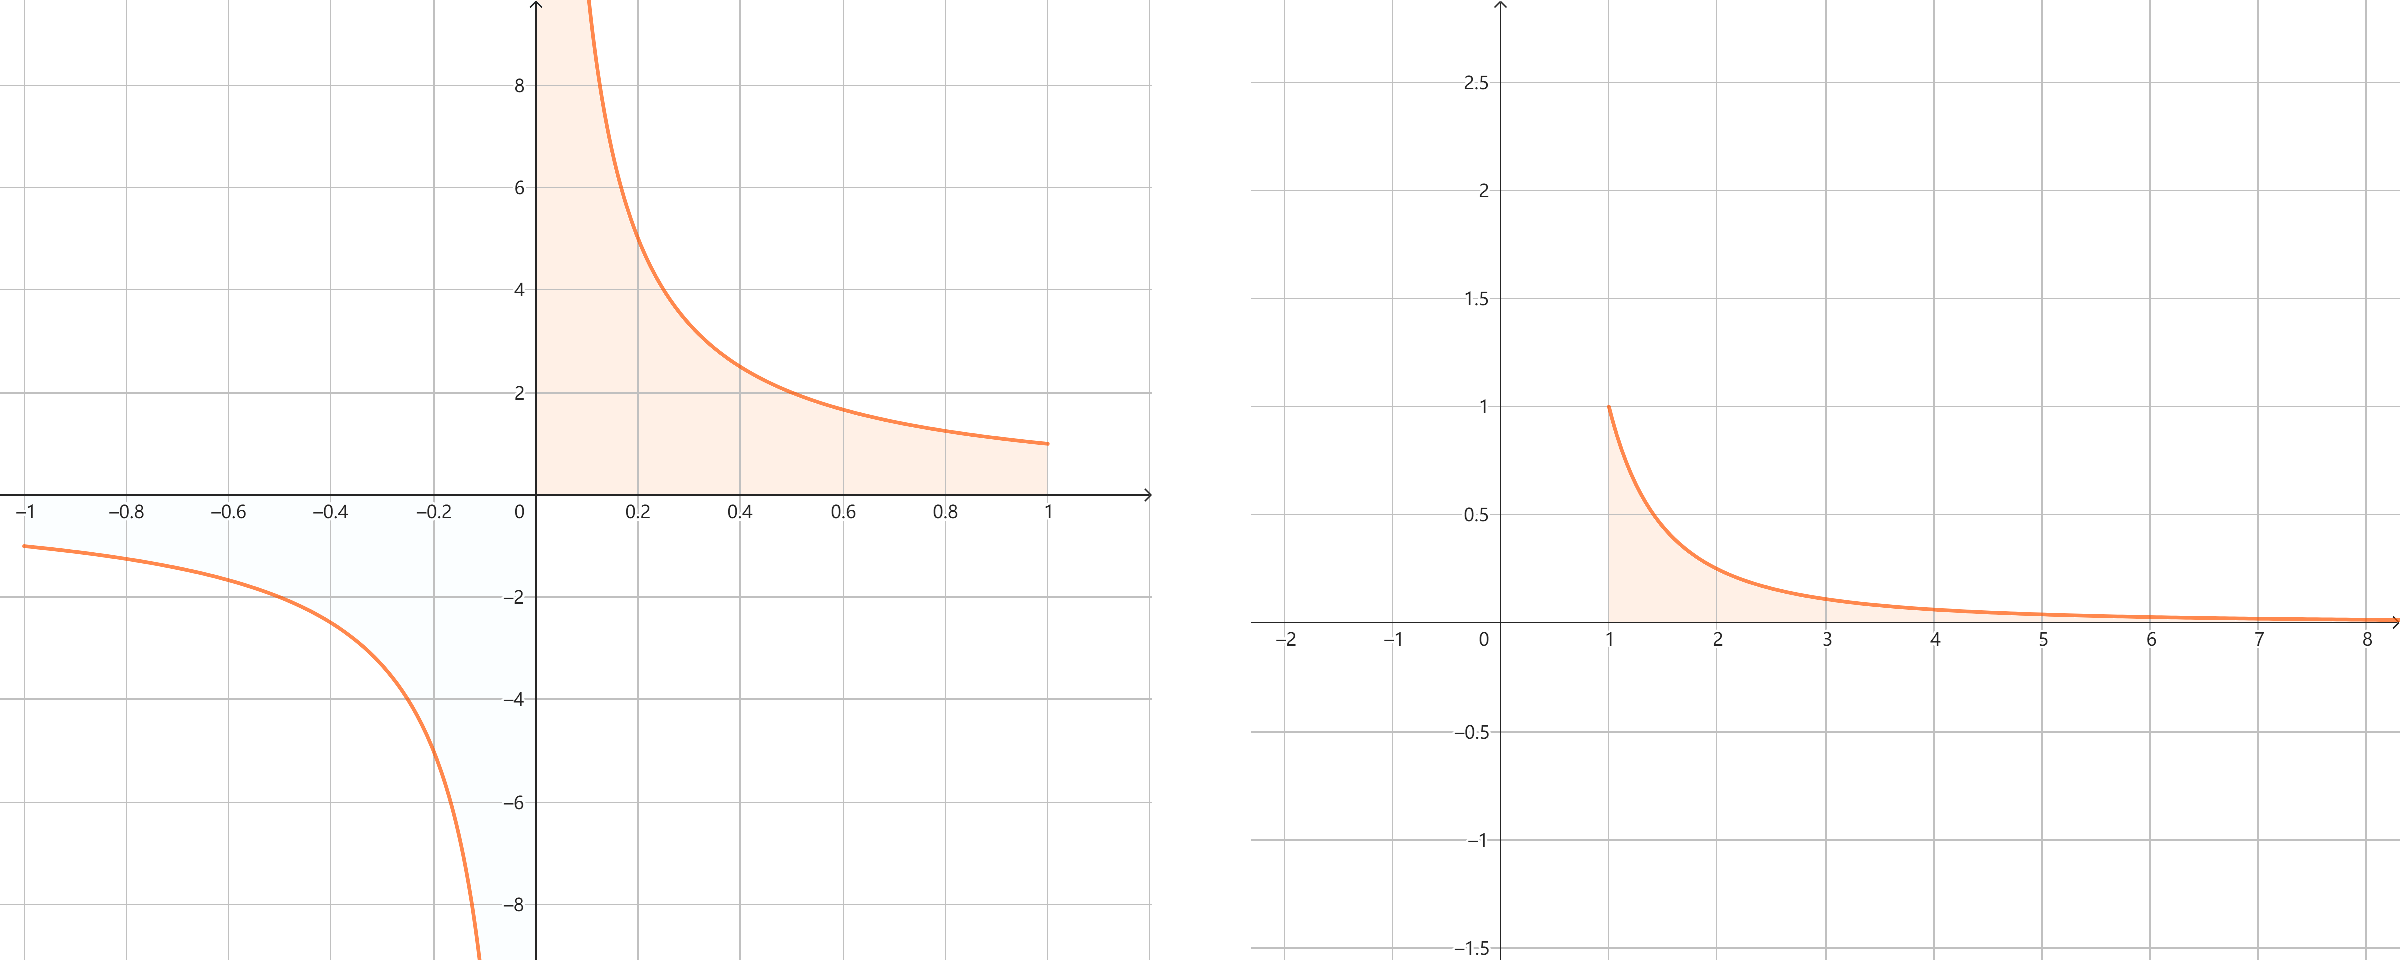
\includegraphics[width=0.9\textwidth]{tu/广义积分1.png}
    \caption*{\texttt{函数}$x\mapsto\frac{1}{x}$(左)、$x\mapsto\frac{1}{x^2}$(右)}
\end{figure}

第一个例子看起来不值得讨论,因为$x\mapsto\frac{1}{x}$甚至不总在$[0;1]$上有定义:$x=0$时,函数无定义。
不过,如果直接看函数的图像,我们能理解这个问题想问什么:如果把积合看作函数与$x$轴之间的图形的面积,那么,
$x\mapsto\frac{1}{x}$这种“无界”的图形是否有面积?

这也是处理一般区间上函数积合时会遇到的问题:闭区间上的连续函数总是有界的,而一般区间上的函数不一定有界。
对于这样的函数,我们能否定义积合呢?

一般来说,以目前的知识,我们无法给任意的函数在任意区间上定义积合。但是,对于一部分“比较好”的函数,我们可以定义积合。

比如,函数$f: x\mapsto\frac{1}{x}$虽然在$[0;1]$上不连续,甚至有未定义的点。但我们可以做一些“修补”。
首先,我们可以给$x=0$处补上定义,比如设$f(0) = 0$。这些工作有助于我们讨论积合的问题,
但不意味着改变函数是否可积的本质。

以上修补过的$f$仍然在$0$处不连续。我们无法直接讨论曲线到$x$轴部分的面积。但我们知道$f$在$(0;1]$上连续。
因此,对任意$a\in(0;1)$,$f$在闭区间$[a;1]$上连续。我们可以求出$f$在$[a;1]$上的面积,然后把$a$趋于$0$。
如果无论$a$以什么方式趋于$0$,面积都趋于一个极限,就定义这个极限为$f$在$[0;1]$上的面积。

首先求$f$在$[a;1]$上的积合:
$$ \int_a^1 f = \ln{1} - \ln{a} = -\ln{a}. $$
这说明$f$在$[a;1]$上的面积是$-\ln{a}$。而$a$趋于$0$时,$-\ln{a}$趋于正无穷。这说明$f$在$[0;1]$上的“面积”是无穷大,
我们说$f$在$[0;1]$上不可积。

第二个例子则比较好理解,因为$f:x\mapsto \frac{1}{x^2}$在$[1;+\infty)$上有定义。我们同样尝试用极限的方式定义函数曲线到$x$轴
的面积。首先求$f$在$[1;a]$上的积合,其中$a>1$:
$$ \int_1^a f = -\frac{1}{a} - (-1) = 1 - \frac{1}{a}. $$
因此$a$趋于正无穷时,$f$在$[1;a]$上的积合趋于$1$。我们说$f$在$[1;+\infty)$上可积。

这样,我们就把积合扩展到定义在一般区间上的连续函数。我们称这种积合为\textbf{广义积合}\footnote{不至于混淆时,也可以简称为积合。}:
\begin{df}
    设函数$f$在半开区间$[a;b)$上连续\footnote{$b$可以是无穷。}。如果当$x$趋于$b$时,$f$在$[a;x]$上的积合总趋于某个极限,
    就说这个极限是$f$在$[a;b)$上的积合,即:
    $$ \int_a^b f = \lian{x\to b^-} \int_a^x f. $$
\end{df}

定义中我们只讨论了区间一端的问题。不过,对于开区间$(a;b)$,我们显然可以先将它截为两段:$(a;c]$、$[c;b)$(其中$c$为区间内任意一点),
然后分别研究这两段是否可积。如果在$(a;c]$、$[c;b)$上都可积,就定义$f$在$(a;b)$上的积合为两段上积合的和。
$$ \int_a^b f = \lian{x\to a^+} \int_x^c f + \lian{x\to b^-} \int_c^x f. $$ 

第一个例子中,我们还“修补”了另一个问题,就是函数在特定点的值的问题。直观来看,函数在单一点是否有定义,或者取不同的值,
不应该改变函数在整个区间上的积合。因为积合是曲线到$x$轴的面积,是一个整体性质。

为此,我们引入分段连续函数的定义:
\begin{df}{\textbf{分段连续函数}}
    设函数$f$在区间$I$上有定义。如果能找到$I$的分割$x_0, x_1, \cdots, x_n$\footnote{其中$x_0$、$x_n$可以是无穷。},
    使得$f$在各个子区间$(x_i;x_{i+1})$上都连续,就说$f$在$I$上(关于该分割)\textbf{分段连续}。
\end{df}
显然,连续函数不论如何分割,总是分段连续的。但也有函数只分段连续而不在整个区间上连续。
比如我们见过的阶梯函数,就是分段连续的不连续函数。

对于分段连续函数,我们可以通过逐段检查,确定它是否可积,并且求出积合。

容易验证广义积合仍然满足积合的基本性质:
\begin{enumerate}
    \item 如果$f$在$I$上可积,且$f$在有限个点以外都大于等于$0$,则其积合大于等于$0$。
    \item 设$a$、$b$、$c$是数轴上的三点,则$\int_a^b f + \int_b^c f = \int_a^c f$。
    \item 设$f$、$g$在$I$上可积,$a, b$为系数,则$ a \int_I f + b \int_I g = \int_I (af + bg) $。
    \item 函数$x\mapsto f\left(\frac{x}{c}\right)$在$[ac; bc]$上的积合,等于$c\int_a^b f$。
    \item 函数$x\mapsto f(x-c)$在$[a+c;b+c]$上的积合,等于$\int_a^b f$。
    \item 如果$f$在区间上的值总介于$m$、$M$之间,那么$m(b - a) \leqslant \int_a^b f \leqslant M(b - a)$。
\end{enumerate}

如果$f$在$I$上有界,那么它在$I$上的广义积合就是它在$I$上的积合。

广义积合与微变也有互逆的关系。比如说,如果$f$在$(a;b]$上可微,且在$a$有右极限,那么:
$$ \int_a^b \partial f = f(b) - \lian{x\to a^+} f.$$
类似地,如果$f$在$[a;b)$上可微,且在$b$有左极限,那么:
$$ \int_a^b \partial f = \lian{x\to b^-} f - f(a).$$

\begin{sk}
    \mbox{} \\
    \indent 1. 假设函数在一点$a$附近(不包括$a$)连续,但在$a$处不连续。这时,不连续的情况可以分成哪几种?其中哪些可以“修补”成连续函数?\\
    \indent 2. 为什么说函数在有限个点上的取值不影响它在区间上的积合?函数在无限个点上的取值是否影响呢?给定区间$I$的子集$D$,
    你认为当$D$满足什么条件的时候,$f$在$D$上的取值会影响它在区间上的积合?\\
    \indent 3. 小明认为,$x\mapsto\frac{1}{x}$在$(0;1]$上的面积是正无穷,在$[-1;0)$上面积是负无穷,所以在$[-1;1]$上面积为$0$。你怎么看?
\end{sk}

\begin{xt}
    \indent 1. 计算以下积合。$a$趋于给定值时,积合是否收敛?\\    
    \begin{align*}
        1).& \int_a^{1} \frac{\ln{x}}{x} , \; a\to 0^+  &2).& \int_1^{a} \e^{-x},  \; a\to +\infty \\[3pt]
        3).& \int_0^{a} \frac{1}{\sqrt{1 - x^2}}, \; a\to 1^-   & 4).& \int_a^{1} \sin{\frac{1}{x}}, \; a\to 0^+ 
    \end{align*}
    \indent 2. 计算以下广义积合。\\    
    \begin{align*}
        1).& \int_0^{+\infty} \frac{1}{x\ln^2{x}} ,  &2).& \int_0^{+\infty} x\e^{-x^2} \\[3pt]
        3).& \int_0^{+\infty} \frac{1}{(1 + \e^{x})^2},  & 4).& \int_0^{+\infty} \frac{\e^{-\sqrt{x}}}{\sqrt{x}}
    \end{align*}
    \indent 3. 仿照极限的定义,具体写出“连续函数在$[1;+\infty)$上可积”的定义。\\

\end{xt}

%%% 
\section{广义可积函数}

下面来看一些经典函数的广义积合。

首先来看函数在某点附近不连续导致的广义积合。

考虑函数$x\mapsto x^{-a}$,其中$a>0$为系数。它在$0$处无定义,在$0$右侧趋于正无穷。它是否在$(0;1]$上可积?

对$t>0$,计算它在$[t;1]$上的积合。$a=1$时,我们知道函数不可积。$a\neq 1$时,
\begin{align*}
    \int_t^1 x^{-a} = \frac{1^{1-a}}{1 - a} - \frac{t^{1-a}}{1 - a} = \frac{1 - t^{1-a}}{1-a} 
\end{align*}

$a<1$时,随着$t$趋于$0$,$t^{1-a}$趋于$0$,因此函数在$(0;1]$上可积,积分为$\frac{1}{1-a}$。

$a>1$时,随着$t$趋于$0$,$t^{1-a}$趋于无穷,因此函数在$(0;1]$上不可积。

考虑函数$x\mapsto \ln{x}$,它在$0$处无定义,在$0$右侧趋于正无穷。它是否在$(0;1]$上有积合?

对$t>0$,计算它在$[t;1]$上的积合。
\begin{align*}
    \int_t^1 \ln{x} = 1\cdot \ln{1} - 1 - (t\cdot\ln{t} - t)= t - t\ln{t} - 1
\end{align*}

$t$趋于$0$时,$t\ln{t}$趋于$0$。因此函数在$(0;1]$上可积,积分为$-1$。

再来看函数在无穷区间上的广义积合。

考虑函数$x\mapsto x^{-a}$,其中$a>0$为系数。它是否在$[1;+\infty)$上可积?

对$t>1$,计算它在$[1;t]$上的积合。

$a=1$时,
\begin{align*}
    \int_1^t x^{-a} = \ln{t} - \ln{1} = \ln{t} 
\end{align*}
$t$趋于无穷时,$\ln{t}$趋于无穷,因此函数在$[1;+\infty)$上不可积。

$a\neq 1$时,它在$[1;t]$上的积合为:
\begin{align*}
    \int_1^t x^{-a} = \frac{t^{1-a}}{1 - a} - \frac{1^{1-a}}{1 - a} = \frac{t^{1-a} - 1}{1-a} 
\end{align*}
$a<1$时,随着$t$趋于无穷,$t^{1-a}$趋于无穷,因此函数在$[1;+\infty)$上不可积。

$a>1$时,随着$t$趋于无穷,$t^{1-a}$趋于$0$,因此函数在$[1;+\infty)$上可积,积分为$\frac{1}{a-1}$。

考虑函数$x\mapsto a^x$,其中$a\in(0;1)$为底数。它是否在$[0;+\infty)$上可积?

对$t>0$,计算它在$[0;t]$上的积合。
\begin{align*}
    \int_0^t a^x = \frac{a^t}{\ln{a}} - \frac{a^0}{\ln{a}} = \frac{a^t - 1}{\ln{a}}
\end{align*}
随着$t$趋于无穷,$a^t$趋于$0$,因此函数在$[0,\infty)$上可积,积分为$-\frac{1}{\ln{a}}$。

\begin{figure}[h] %this figure will be at the right
    \vspace{4pt}
    \centering
    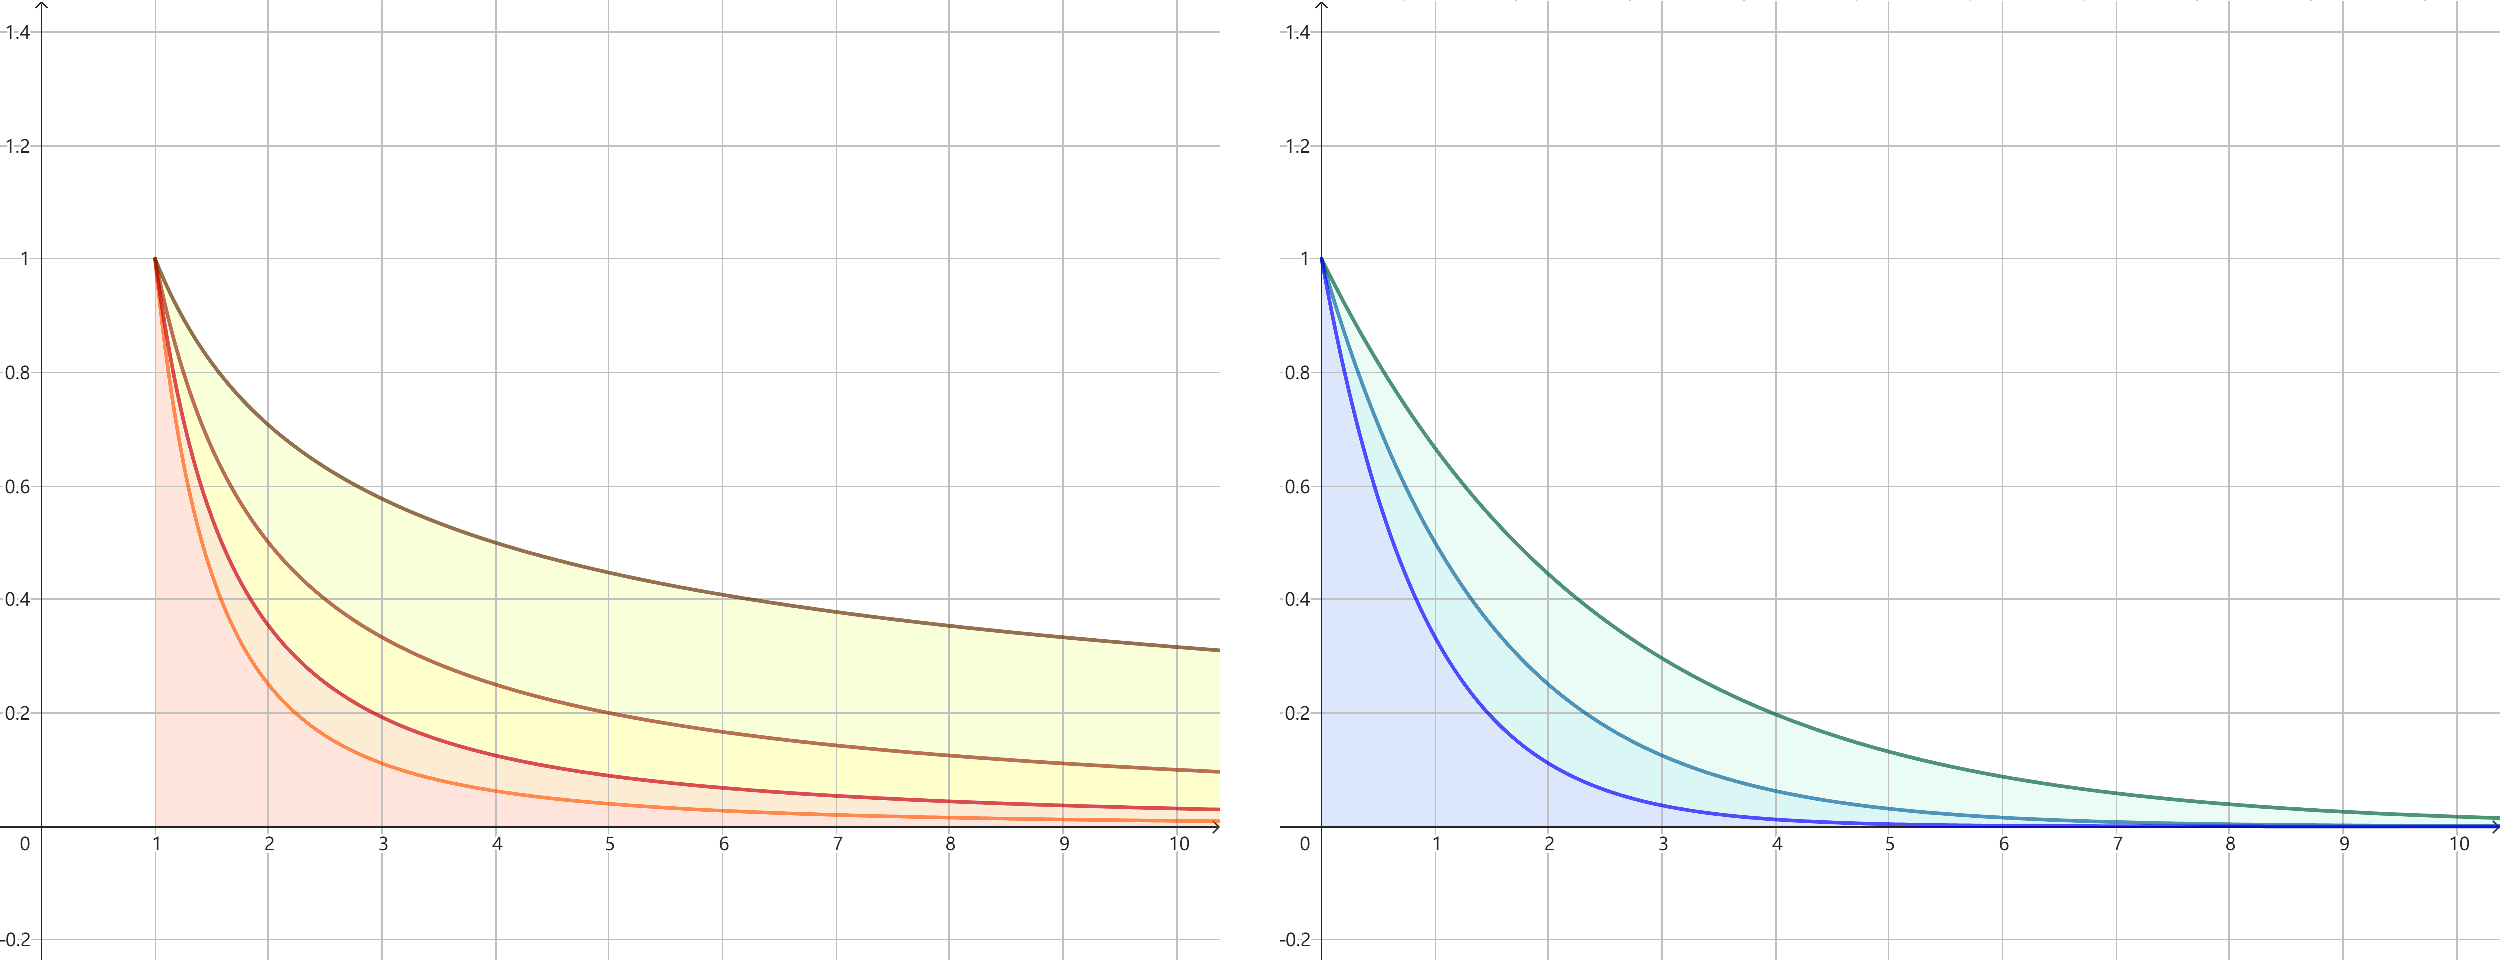
\includegraphics[width=\textwidth]{tu/广义积分2.png}
    \caption*{\texttt{左图:幂函数在}$[1;+\infty)$\texttt{上的面积;右图:指数函数在}$[0;+\infty)$\texttt{上的面积}}
\end{figure}

以上是关于基本的经典函数的讨论,对于更复杂的函数,如何判定它是否广义可积呢?

观察以上的函数在开区间“边缘”的情况,可以发现,造成开区间上面积“无穷”问题的,要么是函数值在开区间端点附近趋于无穷,
要么是开区间为无穷区间——区间长度“无穷”。

我们把前一种情况称为\textbf{无界积合}或\textbf{瑕积合},
把造成问题的端点称\textbf{无界点}或\textbf{瑕点}。而区间为无穷区间的情况,我们称为\textbf{无限积合}。

对于无界积合,直观来说,函数值在瑕点附近急速“爬升”或者“坠落”。
“升”或“落”得越急,曲线到$x$轴的面积就越大;如果“升”或“落”得“太快”,面积就容易变成无穷。

因此,我们可以将函数在无界点附近行为和以上计算过的经典函数进行比较。
如果函数在无界点附近或比可积的经典函数还“慢”,那么可积;如果比不可积的函数还“快”,那么不可积。
而“快慢”程度可以用无穷的阶来具体刻画。

\begin{tm}
    设函数$f$、$g$在区间$I=(a;b]$上分段连续,且在$a$附近同时趋于正无穷。
    \begin{enumerate}
        \item 如果在$a$附近总有$0\leqslant f \leqslant g$,那么只要$g$在$I$上可积,$f$就在$I$上可积。
        \item 如果在$a$附近总有$0\leqslant g \leqslant f$,那么只要$g$在$I$上不可积,$f$就在$I$上不可积。
        \item 如果$f \oveq{a} \Olim{g}$,那么只要$g$在$I$上可积,$f$就在$I$上可积。
        \item 如果$g \oveq{a} \Olim{f}$,那么只要$g$在$I$上不可积,$f$就在$I$上不可积。
        \item 如果$f \oveq{a} \Tlim{g}$,那么$f$在$I$上可积,当且仅当$g$在$I$上可积。
    \end{enumerate}
\end{tm}

举例来说,考虑$(0;1]$上的分段连续函数$f$。如果$f$在$0$点右侧趋于正无穷,那么我们可以将$f$和$x\mapsto x^{-p}$比较。
如果有$p<1$和$r>0$使得$0<x<r$时$f$总受制于$x^{-p}$:
$$ \forall 0<x<r ,\,\,\,\frac{f(x)}{x^{-p}} < M,$$
其中$M$是比值的上界,那么由于$x\mapsto x^{-p}$在$(0;1]$上可积,$f$也在$(0;1]$上可积。

反之,如果$x\mapsto x^{-1}$在$0$右侧附近受制于$f$:
$$ \forall 0<x<r ,\,\,\,\frac{f(x)}{x^{-1}} > M,$$
那么由于$x\mapsto x^{-1}$在$(0;1]$上不可积,$f$也在$(0;1]$上不可积。

再来看无穷积合的情况。
对于无限积合,在无穷远处,如果函数不收敛到$0$,而是收敛到非$0$的数或者趋于无穷,那么显然不可积。
如果函数在无穷远处收敛到$0$,是否就可积呢?

如果函数值(在自变量$x$足够大时)总是正数(或者$0$),那么我们有类似的结论:
\begin{tm}
    设函数$f$、$g$在区间$I=[a;+\infty)$上分段连续。
    \begin{enumerate}
        \item 如果总有$0\leqslant f \leqslant g$,那么只要$g$在$I$上可积,$f$就在$I$上可积。
        \item 如果总有$0\leqslant g \leqslant f$,那么只要$g$在$I$上不可积,$f$就在$I$上不可积。
        \item 如果$0\leqslant f \oveq{+\infty} \Olim{g}$,那么只要$g$在$I$上可积,$f$就在$I$上可积。
        \item 如果$0\leqslant g \oveq{+\infty} \Olim{f}$,那么只要$g$在$I$上不可积,$f$就在$I$上不可积。
        \item 如果$0\leqslant f \oveq{+\infty} \Tlim{g}$,那么$f$在$I$上可积,当且仅当$g$在$I$上可积。
    \end{enumerate}
\end{tm}

考虑$[1;+\infty)$上的分段连续函数$f\geqslant 0$。我们可以将$f$和$x\mapsto x^{-p}$比较。
如果有$p>1$和$A>0$使得$x>A$时$f$总受制于$x^{-p}$:
$$ \forall x>A ,\,\,\,\frac{f(x)}{x^{-p}} < M,$$
其中$M$是比值的上界,那么由于$x\mapsto x^{-p}$在$[1;+\infty)$上可积,$f$也在$[1;+\infty)$上可积。

反之,如果$x\mapsto x^{-1}$在$0$右侧附近受制于$f$:
$$ \forall x>A ,\,\,\,\frac{f(x)}{x^{-1}} > M,$$
那么由于$x\mapsto x^{-1}$在$[1;+\infty)$上不可积,$f$也在$[1;+\infty)$上不可积。

以上讨论中我们加上了函数大于等于$0$的条件。如果函数值可正可负时,情况更加复杂。
我们可以把无限积合与可数个数求和——也就是级数——的情况类比。
讨论级数收敛时,我们将级数分为正项级数和一般的级数,并引入了级数的绝对值、绝对收敛和相对收敛的概念。

对于无限积合,我们引入\textbf{绝对可积}的概念。
对于定义在区间$I$上的函数$f$,如果它的绝对值$|f|: x\mapsto |f(x)|$在$I$上可积,就说$f$绝对可积;
否则就说$f$\textbf{相对可积}。

在$I$上绝对可积的函数,一定相对可积,但反之则不一定。

要注意的是,如果函数在无穷远处没有极限,并不能说明它可积或不可积。比如说,我们可以在足够远处给函数加上一些“小尖刺”。
每个“小尖刺”的面积都很小,不影响可积,但“刺尖”的函数值可以很大,甚至趋于无穷。

具体来说,我们制作这样的“尖角函数”:
\begin{align*}
    f: [0;1] &\rightarrow \mathbb{R} \\
x \;&\mapsto \begin{cases}
    2x & 0\leqslant x \leqslant \frac{1}{2} \\
    1 - 2x & \frac{1}{2} < x \leqslant 1
\end{cases} 
\end{align*}
这个函数的图像是平放在$x$轴上的等腰三角形。它的左端和$0$对齐,底和高都是$1$。我们可以将它拉伸放缩为“尖刺”:
\begin{align*}
   [a;a+b] &\rightarrow \mathbb{R} \\
    x \;&\mapsto h\cdot f\left(\frac{x-a}{b}\right)
\end{align*}
这个函数的图像也是$x$轴上的等腰三角形,只不过底边是$x$轴上的线段$[a;a+b]$,底长为$b$,高为$h$。

取一个在$[1;+\infty)$上可积的非负函数,比如$\displaystyle f_0: x\mapsto \frac{1}{x^2}$。在足够远的地方放置这些“尖刺”,得到以下函数:
$$
g: x\mapsto \begin{cases}
    \displaystyle f_0(x) + 2n f\left(n^3(x - n)\right) & \mbox{如果}\; x \in \left[n;n+\frac{1}{n^3}\right],\; n\in\mathbb{Z}^+ \\
    f_0(x) & \mbox{其他的}\;x
\end{cases}
$$
对任意正整数$n$,函数$g$在区间$\left[n;n+\frac{1}{n^3}\right]$上叠加放置了底边为$\frac{1}{n^3}$,高为$2n$的等腰三角形。它的面积为$\frac{1}{n^2}$。

因此,相对于$f_0$,$g$的面积增加不超过$\displaystyle \sum_{n\geqslant 1} \frac{1}{n^2}$。而$\displaystyle \sum_{n\geqslant 1} \frac{1}{n^2}$是收敛的级数,所以函数$g$也是可积乃至绝对可积的。
然而,$g$的函数值在$n+\frac{1}{2n^3}$处可以达到$2n$,因此没有上限,随着$n$的增大而趋于无穷。

从这个例子可以看出,无限积合的判断比无界积合、级数收敛的判断更复杂。这是由实数集的不可数特性和函数的复杂性决定的。

\begin{sk}
    \mbox{} \\
    \indent 1. 总结非负连续函数的无限积合和正项级数的收敛的相似性。\\
    \indent 2. 为什么讨论无界积合时,没有考虑函数值的正负性?\\
    \indent 3. 广义积合可以看作对函数的积合求极限。是否可以先对函数求极限,再求积合?这两种操作是否等价?\\
    \indent 4. 连续函数在无穷远处不收敛到$0$,是否一定不可积?
\end{sk}

\begin{xt}
    \mbox{} \\
    \indent 1. 以下函数是否在$\mathbb{R}^+$上可积?\\    
    \begin{align*}
        1)\;\;& \frac{1}{x\ln^2{x}} ,  &2)\;\;& \frac{\e^{-x^2}}{\sqrt{x}}, \\[3pt]
        3)\;\;& \sin{\frac{1}{x}},  & 4)\;\;& \frac{1}{\e^x  - 1}.
    \end{align*}
    \indent 2. 以下积合是否存在?\\    
    \begin{align*}
        1)\;\;& \int_2^{+\infty} \frac{1}{\sqrt{x(x - 1)(x - 2)}},  &2)\;\;& \int_0^{\frac{\pi}{2}} \frac{1}{\sin{x}\cos{x}(1 - \e^{-x})}, \\[3pt]
        3)\;\;& \int_0^{1} \frac{\ln{x}}{(1 - x^2)^{\frac{3}{2}}} , & 4)\;\;& \int_0^{\pi} \frac{1}{\sqrt{\sin{x}}}.
    \end{align*}
    \indent 3. $f$是$[1;+\infty)$上的分段连续函数。\\
    \indent 3.1. 证明:如果有正实数$a>1$使得$\lian{t\to+\infty} t^a f(t) = 0$,那么$f$在$[1;+\infty)$上绝对可积。\\
    \indent 3.2. 证明:如果有正实数$c$使得$\lian{t\to+\infty} t f(t) \geqslant c$,那么$f$在$[1;+\infty)$上不可积。\\
    \indent 4. $f$是$(0;1]$上的分段连续函数。\\
    \indent 4.1. 证明:如果有正实数$a<1$使得$\lian{t\to 0^+} t^a f(t) = 0$,那么$f$在$(0;1]$上绝对可积。\\
    \indent 4.2. 证明:如果有正实数$c$使得$\lian{t\to 0^+} t f(t) \geqslant c$,那么$f$在$(0;1]$上不可积。\\
    \indent 5. 当$a$取什么值的时候,以下带参数$a$的函数在$\mathbb{R}^+$上可积?\\
    \begin{align*}
        1)\;\;& \frac{\ln{x}}{x^a} ,  &2)\;\;& \frac{\e^{-x} - 1}{x^a}, \\[3pt]
        3)\;\;& \frac{x - \sin{x}}{x^a},  & 4)\;\;& \frac{\arctan{x}}{x^a}. 
    \end{align*}
    \indent 6. 设$f$是$\mathbb{R}^+$上的连续可积函数。\\
    \indent 6.1. 设$\{x_n\}$、$\{y_n\}$为两个趋于正无穷的数列。证明:
    $$ \lian{n\to+\infty}\int_{x_n}^{y_n} f = 0. $$
    \indent 6.2. 证明:$\e^{-t\sin{t}}$在$\mathbb{R}^+$上不可积。

\end{xt}

\section{积合的应用}

和我们已经学习过的大多数数学概念一样,积合也来自实际生活、生产中的需要。使用积合作为工具,可以解决许多实践中的问题。
下面我们来看一些典型的例子。

\begin{et}{\textbf{曲边图形的面积}}\\
    计算以下曲线图形的面积。\\
    \indent 1. 正弦函数$x\mapsto \sin{x}$在$[0;\pi]$上到$x$轴的面积。 \\
    \indent 2. 幂函数$x\mapsto x^n$在$[0;1]$上到$x$轴的面积。\\
    \indent 3. 二次函数$x \mapsto \frac{4x^2}{\pi^2}$与正弦函数围成的图形的面积。
\end{et}

\begin{so}
    \indent 1. 按照定义,这个面积$S$就是正弦函数在$[0;\pi]$上的积合。计算可知:
    \begin{align*}
        S &= \int_{0}^{\pi} \sin{x} = -\cos{\pi} - (-\cos{0}) \\
        &= 1 + 1 = 2
    \end{align*}

    \indent 2. 按照定义,这个面积$S$就是幂函数在$[0;1]$上的积合。计算可知:
    \begin{align*}
        S &= \int_{0}^{1} x^n = \frac{1^{n+1}}{n+1}- \frac{0^{n+1}}{n+1} \\
        &= \frac{1}{n+1}
    \end{align*}

    \indent 3. 直观来看,围成的图形上侧边界为正弦曲线,下侧为二次函数的曲线。
    换句话说,围成的面积就是正弦曲线到$x$轴的面积减去二次函数曲线到$x$轴的面积,也就是两者在交点之间的积合之差。

    \indent 分析两条曲线,可知它们交点的坐标为$(0,\;0)$和$\left(\frac{\pi}{2},\;1\right)$。也就是说,围成的面积$S$可以写为:
    \begin{align*}
        S &= \int_{0}^{\frac{\pi}{2}} \sin{x} - \int_{0}^{\frac{\pi}{2}} \frac{4x^2}{\pi^2} \\ 
        &= -\left(\cos{\frac{\pi}{2}} - \cos{0}\right) - \frac{4}{3\pi^2} \left( \left( \frac{\pi}{2} \right)^3 - 0^3 \right) \\
        &= 1 - \frac{\pi}{6}
    \end{align*}
\end{so}

要注意的是,积合表示的是函数曲线到$x$轴的有向面积。如果一个函数在定义区间上有正有负,
那么它在区间上的积合表示它在$x$轴上方部分的面积减去$x$轴下方部分的面积的差。反之,如果我们不考虑面积的正负,
那么我们需要计算函数绝对值的积合。

积合不但能表示平面上曲边图形的面积,还能用来处理立体空间中的概念。

\begin{et}{\textbf{旋转体的体积}}\\
    立体空间$Oxyz$中,设有$xOy$平面上的连续函数曲线:$y = f(x)$,它在区间$[a;b]$上的部分绕$x$轴旋转,计算得到的旋转体的体积。
    以此计算圆锥和球的体积。
\end{et}

\begin{so}
    为方便起见,我们首先考虑函数$f$在区间$[a;b]$上不小于$0$的情况。

    考虑$f$为常函数$x\mapsto r$的情况,这时的旋转体是底面半径为$r$的圆柱,因此体积为$\pi r^2 (b - a)$。因此,仿造从函数曲线到$x$轴的面积来定义积合的方法,
    我们可以定义$[a,b]$上的连续函数曲线对应的旋转体体积。与通过函数曲线到$x$轴的面积构造积合的唯一不同是,
    常函数$x\mapsto r$不再对应矩形面积$r(b - a)$,而是对应圆柱体积$\pi r^2 (b - a)$。
    
    对区间作分割$(x_0, x_1, \cdots, x_n)$,分割出的每个小区间$[x_{i-1};x_i]$上取样$c_i$,用半径为$c_i$,
    高为$x_i - x_{i-1}$圆柱近似表示旋转体在$[x_{i-1};x_i]$部分的体积,于是旋转体的体积近似表示为:
    $$ \sum_{i=1}^n (x_i - x_{i-1}) \pi f^2(c_i) $$

    从另一个角度来看,如果我们考虑函数$g: x\mapsto \pi f^2(x)$,那么同样的分割下,旋转体的体积近似等于$g$的取样和。
    因此,当分割越来越精细,上述取样和趋于$g$的函数曲线到$x$轴的面积,也就是旋转体的体积。
    换句话说,$[a;b]$上的连续函数$f$的曲线绕$x$轴旋转得到的旋转体的体积,就是$\pi f^2$在$[a;b]$上的积合:
    $$ V = \int_a^b \pi f^2(x) = \pi \int_a^b f^2(x). $$

    如果函数$f$在区间上有正有负,那么可以考虑它的绝对值函数$x\mapsto |f(x)|$。它绕$x$轴旋转得到的旋转体和$f$是一样的。
    因此,旋转体的体积是$ \pi \int_a^b |f(x)|^2$,也就是$ \pi \int_a^b f^2(x)$。
    这说明上述公式对区间$[a;b]$上的任何连续函数都适用。

    以圆锥为例。考虑以$x = h$上的圆$y^2 + z^2 = r$为底,以$y = \frac{rx}{h}$为母线的圆锥。这时的函数为$x\mapsto \frac{rx}{h}$,
    所以按上述公式,圆锥体积为:
    $$ V = \int_0^h \pi \frac{r^2x^2}{h^2} = \frac{\pi r^2}{h^2}\cdot \frac{h^3 - 0^3}{3} = \frac{\pi r^2h}{3}. $$

    再来看球体。考虑以原点为圆心,半径为$r$的球。它可以看作$[-r;r]$上的函数$x\mapsto \sqrt{r^2 - x^2}$对应的旋转体的体积。
    所以按上述公式,球的体积为:
    \begin{align*}
        V &= \int_{-r}^r \pi \left(\sqrt{r^2 - x^2}\right)^2 = \pi \int_{-r}^r \left(r^2 - x^2\right) \\
        &= \pi \left(r^2(r - (-r)) - \frac{r^3 - (-r)^3}{3}\right) = \pi \left(2r^3 - \frac{2r^3}{3}\right) \\
        &= \frac{4\pi r^3}{3}.
    \end{align*}
\end{so}

同样的思考方式,可以用来计算曲线的长度。我们曾经(不严谨地)定义曲线长度为曲线上的点连成的折线长度的上极限。
使用积合的概念可以更好地理解和计算曲线的长度。

\begin{et}{\textbf{光滑曲线的长度}}\\
    设实函数$f$在区间$[a;b]$上连续可微,计算它在$[a;b]$上的长度。
    并据此计算$x\mapsto x^2$在区间$[0;1]$上的长度。    
\end{et}

\begin{so}
    考虑$f$在区间上的某个分割$(x_0, x_1, \cdots, x_n)$,在分割很细的时候,
    我们可以近似地把每一段上的曲线看作连接两端得到的线段,因此曲线近似于一条折线。
    这些折线的长度和小于曲线长度。但我们可以想象,随着分割越来越精细,折线的长度和将趋于某个上极限,这个极限就是曲线的长度。

    然而,这个上极限不总是存在。对我们所知的一些曲线,比如圆弧来说,上极限存在。
    但也有一些曲线,当我们以某种方式分割时,随着分割越来越精细,折线的长度和将趋于正无穷。
    我们无法给这种曲线定义长度,一般认为它们无限长。上极限存在的曲线称为\textbf{可求长曲线}。

    对连续可微函数来说,我们可以证明上述的上极限存在。函数$f$连续可微,因此在区间$[x_{i-1};x_i]$上,
    折线的长度$s_i$可以用$\partial f$来近似表示:
    \begin{align*}
        s_i^2 &= (x_i - x_{i-1})^2 + (f(x_i) - f(x_{i-1}))^2 = (x_i - x_{i-1})^2\left( 1 + \left(\frac{f(x_i) - f(x_{i-1})}{x_i - x_{i-1}}\right)^2\right) \\
        s_i &= (x_i - x_{i-1})\sqrt{1 + \left(\frac{f(x_i) - f(x_{i-1})}{x_i - x_{i-1}}\right)^2} \\
        &= (x_i - x_{i-1})\sqrt{1 + \left(\partial f(x_{i-1}) + \olim{1}\right)^2}\\
        &= (x_i - x_{i-1})\sqrt{1 + \partial f^2(x_{i-1}) + \olim{1}}\\
        &= (x_i - x_{i-1})\left(\sqrt{1 + \partial f^2(x_{i-1})} + \olim{1}\right)
    \end{align*}
    其中的无穷小$\olim{1}$是关于$x_i - x_{i-1}$的函数,当$x_i - x_{i-1}$趋于$0$时趋于$0$。

    对$h$\dash 分割来说,按照定义,所有小区间的长度都小于$h$,因此,$h$趋于$0$时,所有的$x_i - x_{i-1}$都趋于$0$,因此以上的$\olim{1}$都趋于$0$。
    因此$h$趋于$0$时,$h$\dash 分割下所有折线的长度和为:
    \begin{align*}
        l &= \sum_{i=0}^{n-1} s_i = \sum_{i=1}^{n} (x_{i+1} - x_{i})\left(\sqrt{1 + \partial f^2(x_{i-1})} + \olim{1}\right) \\
        &= \sum_{i=1}^{n} (x_{i+1} - x_{i})\sqrt{1 + \partial f^2(x_{i-1})} + \sum_{i=1}^{n} (x_{i+1} - x_{i})\olim{1} \\
        &= \sum_{i=1}^{n} (x_{i+1} - x_{i})\sqrt{1 + \partial f^2(x_{i-1})} + (b - a)\olim{1} \\
        &= \sum_{i=1}^{n} (x_{i+1} - x_{i})\sqrt{1 + \partial f^2(x_{i-1})} + \olim{1}
    \end{align*}
    我们把$l$拆成了两项的和。当分割不断变得更精细,$h$趋于$0$时,第二项$\olim{1}$趋于$0$,
    而第一项则与函数$g: \;x\mapsto \sqrt{1 + \partial f^2(x) }$的取样和一样。
    这说明:如果$g$在区间上可积,那么折线长度和$l$就趋于它的积合:
    $$ \int_a^b \sqrt{1 + \partial f^2(x) }. $$
    由于我们设定$f$连续可微,因而$\partial f$与$x\mapsto \sqrt{1 + x^2}$都是连续函数,
    故它们的复合函数$g$也是连续函数,因此可积。于是以上积合存在,并且是折线长度和$l$的极限。
    我们称它为连续可微函数$f$在$[a;b]$上的长度。以$x\mapsto x^2$为例,可以计算它在$[0;1]$上的长度。 
    \begin{align*}
        l &= \int_0^1 \sqrt{1 + (2x)^2 } = \int_0^1 \sqrt{1 + 4x^2 } \\
        &= \frac{1\cdot \sqrt{1 + 4\cdot 1^2} - 0\cdot \sqrt{1 + 4\cdot 0^2}}{2} + \frac{1}{4}\left( \ln{\left(1 + \frac{\sqrt{1 + 4\cdot 1^2}}{2}\right)} -  \ln{\left(0 + \frac{\sqrt{1 + 4\cdot 0^2}}{2}\right)}\right) \\
        &= \frac{\sqrt{5}}{2} + \frac{\ln{\left(2 + \sqrt{5}\right)}}{4}.
    \end{align*}

\end{so}

从以上的例子来看,科学研究和生产实践中,如果我们想使用积合作为工具,计算某个量$Q$在一段区间$[a;b]$上的和,而$Q$满足以下条件:
\begin{enumerate}
    \item $Q$是由区间的起点和终点决定的量:它在任意区间$[u;v]$上的值可以表示为$Q(u,\, v)$。
    \item $Q$在区间$I$上可加,也就是说,只要$u < v < w \in I$,就有:
            $$ Q(u, v) + Q(v, w) = Q(u, w).$$
\end{enumerate}
那么,可以用类似的方法来处理:
\begin{enumerate}
    \item 确定$Q$所对应的某个函数$g$,使得在任意区间$[u;u + \di{u}]$上有:
    $$Q(u, \, u + \di{u}) = g(t)\di{u} + \olim{\di{u}},$$
    其中$t\in [u;u+ \di{u}]$是某种取样结果\footnote{实际上$g$也可以是关于$u$、$v$或$\di{u}$的函数。},$\olim{\di{u}}$是$\di{u}$在$0$处的高阶无穷小。
    \item 对任意$h$\dash 分割$(x_0, x_1, \cdots, x_n)$,论证取样和
    $$Q(a, b) = \sum_{i=1}^n Q(x_{i-1},\, x_i)$$
    可以写为:
    $$Q(a, b) = \sum_{i=1}^n g(t_i)(x_i - x_{i-1}) + \olim{1},$$
    其中$\olim{1}$是$h$在$0$处的无穷小。
    \item 论证$g$在$I$上可积。从而随着分割不断精细,以上取样和趋于$g$在区间$I$上的积分。因此$Q(a, b)$的值就等于$g$在区间$I$上的积分。
\end{enumerate}
这种方法源自历史上对随着时间或路径变化的物理量的累积效果的研究,称为\textbf{微积分法}或\textbf{微元法}。
历史上,通常把在微小区间中找到函数$g$和近似关系$Q(u,u + \di{u}) \approx g(t)\di{u}$的过程称为\textbf{微分},
把微小区间$[u;u+\di{u}]$上的累积量$\di{Q} = Q(u, u + \di{u}) \approx g(t)\di{u}$称为\textbf{微元},
把随后论证取样和关系的过程称为\textbf{积分}。总的过程可以概括为“求微元,先微分,后积分”。

% 《微元法的一个理解与思考》梁东颖,晁绵涛, 应用数学进展, 2023, 12(5), 2187-2192 DOI: 10.12677/aam.2023.125223
% https://www.hanspub.org/journal/aam https://doi.org/10.12677/aam.2023.125223

\begin{xt}
    \mbox{} \\
    \indent 1. 证明以下的体积公式。\\
    \indent 1.1. 椭圆$\displaystyle\frac{x^2}{a^2} + \frac{y^2}{b^2} = 1$绕$x$轴旋转得到的旋转体的体积为:
    $$ V = \frac{4\pi}{3} ab^2. $$
    \indent 1.2. 圆$x^2 + (y - b)^2 = a^2$绕$x$轴旋转得到的旋转体的体积为:
    $$ V = 2\pi^2 a^2 b. $$
    \indent 2. 计算以下旋转体的体积。\\
    \indent 2.1. 将直线$\frac{x}{3} + y = 2$与$x$轴、$y$轴围成的三角形绕$x$轴旋转,得到的旋转体的体积。\\
    \indent 2.2. 曲线$y^2 = x$与直线$x=4$围成的图形绕$x$轴旋转,得到的旋转体的体积。\\
    \indent 2.3. 曲线$y = \cos{x}$在$\displaystyle\left[-\frac{\pi}{2};\frac{\pi}{2}\right]$上的曲线绕$x$轴旋转得到的旋转体的体积。
\end{xt}


\chapter{方程与空间}

\begin{ex}
    某城的城墙是正圆的。东南西北各有城门。甲从北门往北直走$160$步,乙从西门往西直走$60$步后,
    恰能相互看见。问圆城半径几何? % 240
\end{ex}

\begin{wrapfigure}[8]{r}{0.36\textwidth} %this figure will be at the right
    \vspace{-30pt}
    \flushright
    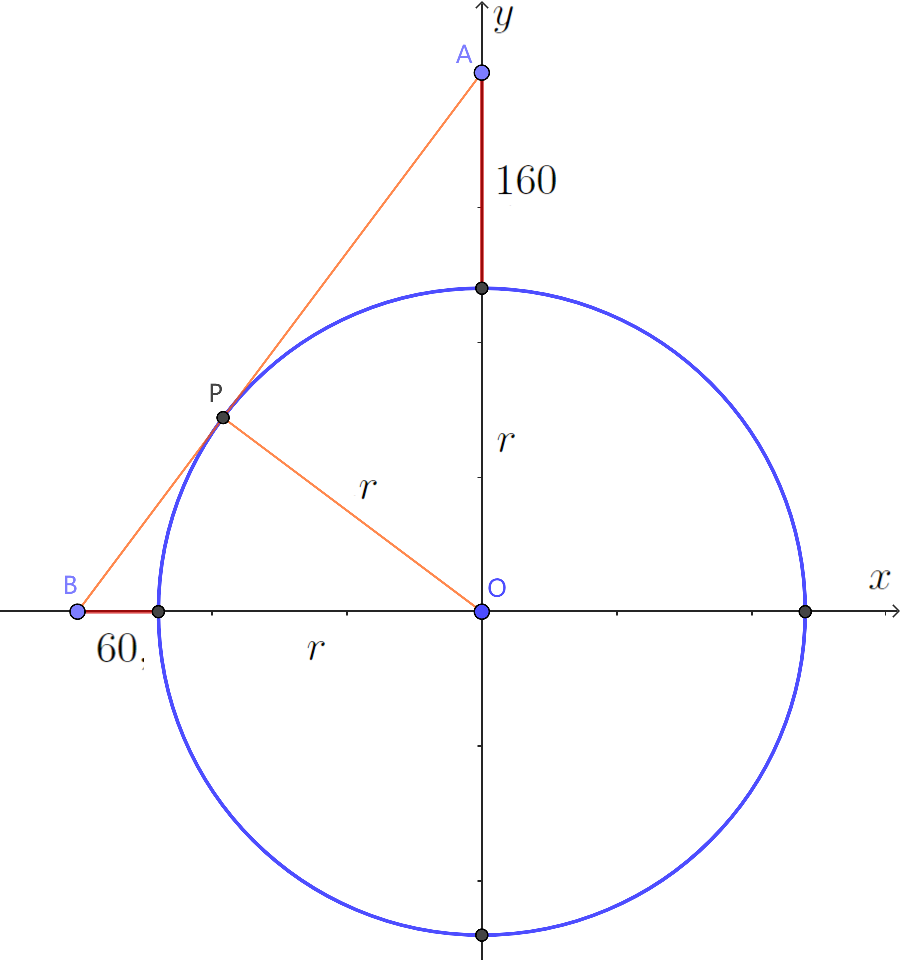
\includegraphics[width=0.35\textwidth]{tu/整式方程1.png}
\end{wrapfigure}

这个问题是一个实际的测量问题。我们把它转为数学问题。

如图,根据题目条件,可以将城墙看作圆形。记圆心为$O$,以$O$为原点,东西、南北向各作坐标轴,得到直角坐标系$xOy$。
城门就是坐标轴与圆形的交点。

设圆的半径为$r$,则北门、西门的坐标分别是$(0, \,\, r)$、$(-r, \,\, 0)$。
而按题目描述,甲乙恰能相望时,分别位于点$A:(0, \,\, r+160)$、$B:(-r-60, \,\, 0)$。

连接$AB$,则$AB$与圆相切。设切点为$P$。$\triangle AOB$、$\triangle AOP$是直角三角形,
且
$$ \triangle APO \simeq \triangle AOB.$$
于是有
$$ \frac{|AO|}{|PO|} = \frac{|AB|}{|OB|}.$$
$|AO| = r+160$,$|PO| = r$,$|OB| = r + 60$,而根据勾股定理,
$$ |AB|^2 = |AO|^2 + |OB|^2,$$
于是:
$$ |AO|^2 |OB|^2 = \left(|AO|^2 + |OB|^2\right) |PO|^2 $$
即:
$$ (r+160)^2 (r+60)^2 = \left((r+160)^2 + (r+60)^2\right) r^2 $$
两边展开化简,得到:
% $$ (r^2 + 2ar + a^2)(r^2 + 2br + b^2) $$
% $$ r^4 + 2(a + b)r^3 + (4ab + a^2 + b^2)r^2 + 2ab(a + b)r + a^2b^2 $$
% $$ 2r^4 + 2(a + b)r^3 + (a^2 + b^2)r^2 $$
$$ r^4 - 3\dlim{8400} r^2 - 422\dlim{4000} r - 9216\dlim{0000} = 0. $$

\begin{ex}
  % 线性方程组例子
  考虑化学反应:氨气和氧气反应,生成一氧化氮和水。其化学反应方程式为:

\begin{center}
  \ce{NH3 + O2 ->T[催化剂] NO + H2O}
\end{center}

  配平这个化学反应式。
\end{ex}

配平化学反应的方程式,主要是求出每种物质参与反应的量。配平后的方程式应该如以下形式:

\begin{center}
    \ce{{\color{blue}a} NH3 + {\color{blue}b} O2 = {\color{blue}c} NO + {\color{blue}d} H2O}
\end{center}

其中的$a, b, c, d$是配平的系数。

化学反应满足物质守恒和电荷守恒。从每种物质的守恒出发,可以得到以下方程:
$$ \qquad \qquad \qquad \qquad \left\{
    \begin{array}{rll}
a &= c &\qquad \qquad \qquad \qquad (N) \\
3a &= 2d &\qquad \qquad \qquad \qquad (H) \\
2b &= c + d &\qquad \qquad \qquad \qquad (O) \\
\end{array}
\right. 
$$
这是由三个方程构成的方程组,涉及$a, b, c, d$四个未知数。通过移动,可以让各个方程右边不含未知数:
$$\left\{
    \begin{array}{rrrrl}
\phantom{0}a &\phantom{+ 0b} &- \phantom{0}c &\phantom{+ 0b}\, &= 0  \\
3a &\phantom{+ 0b} &\phantom{- 0c} &- 2d\, &= 0  \\
\phantom{0a} &\phantom{+ }\quad 2b &- \phantom{0}c &- \phantom{0}d\, &= 0  
\end{array}
\right. 
$$

\begin{ex}
    电源回路中串联了一个电容器和一个电阻器,它们的电容和电阻分别是$C$和$R$。初始状态下,回路电压为$U$。
    关闭电源后,电容开始放电。描述电容器两端的电势差$u$随时间变化的过程。
\end{ex}

断电后,回路中只有电容器和电阻器。考虑任意时刻$t$,回路的电势关系为:
$$ u(t) + I(t)R = 0.$$
其中$I(t)$是回路中的电流,它由电容放电得到。
按定义,放电时的电流为电量关于时间的变化率,而电量与电容器两端的电势差成正比,即:
$$ I(t) = \partial Q(t) = \partial (Cu(t)) = C\partial  u(t).$$
因此:
$$ u(t) + RC\partial  u(t) = 0.$$

以上的例子中,我们从实际问题出发,得到了关于未知量的方程。这种方法是使用数学知识解决实际问题的主要方法。
将实际问题转为数学问题,称为建立数学模型,简称建模。
数学模型就是把实际问题中的某些形状、数量关系用数学中的对象代替,用数学对象模拟实际情形。解决了数学模型中的问题,
就对应地解决了实际中的问题。

把实际问题转化为数学问题,需要多方面的考虑,我们不打算在此详细介绍。以下我们主要关心建模得到的数学问题。
从以上两个例子可以看到,建模得到的数学问题,经常以方程的形式出现。
方程可以看作是实际问题中的约束条件转化到数学的结果。

从数学的角度来看,方程就是指示某个集合的子集的方式。
我们首先假定未知量可以在某个集合(比如$\mathbb{R}$)中取值,而方程告诉我们未知量需要满足的约束条件。
约束条件对应着集合的子集,而解方程就是找出这个特定的子集,称为方程的解。

举例来说,给定一元一次方程
$$ 2x + 1 = 0$$
我们首先假设未知量$x$可以在$\mathbb{R}$中取值,那么这个方程告诉我们,$x$满足约束条件:$2x+1=0$。
它对应的解集是$\mathbb{R}$的子集:
$$ \left\{ x\in\mathbb{R} \, | \, 2x + 1 = 0 \right\} $$
而解这个方程,就是明确这个子集到底是什么。在这里,解集是$\{-0.5\}$。

一般来说,我们在实际问题中寻找相等关系。建模后,相等关系就转化为方程。方程的未知量就是问题中我们关心的量,
而解方程就是找出它的值所属的子集,也就是它可能的取值。

在第一个例子中,我们关心的是圆城的半径$r$。$r$是正实数。建模后,我们得到$r$满足的方程。解方程就得到$r$可能的取值。

在第二个例子中,我们关心的是配平的系数。建模后,我们得到系数满足的方程组。解方程组就得到系数可能的取值。

在第三个例子中,我们关心的是电容器两端的电势差$u$。$u$是关于时间$t$的函数。
建模后,我们得到$u$满足的方程。解方程就得到$u$可能的取值。

\section{整式方程}

第一个例子里,我们得到的方程是关于未知量$r$的。方程一边是$0$,另一边是$r$的整式。我们把这样的方程称为整式方程。

整式方程的未知量可以是一个,也可以是多个,分别称为一元整式方程和多元整式方程。方程中,未知量用“元”称呼。
整理后,整式方程总可以写成:
$$ P(x_1, \cdots ,x_m) = 0.$$
其中$P$是某个整式,$x_1, \cdots ,x_m$是未知量。整式方程可以按照整式$P$的元数和次数区分。
比如,第一个例子里的整式是一元四次整式,就说它对应的方程是一元四次方程。我们已经学习过一元一次方程和一元二次方程。

很多时候,方程的数量可以不止一个,对应多个约束条件,称为方程组。我们已经学习过二元一次方程组。
广义上来说,单个方程也可以视作方程组。

\subsection{一元整式方程}

第一个例子中的方程是一元四次方程。如何解这样的方程呢?

对于一元一次方程和一元二次方程,我们有关于系数的公式,
通过加减乘除和开方,得到方程的解。这种公式称为一元整式方程的\textbf{求根公式}。
一元三次方程和一元四次方程也有求根公式,但比一次和二次方程复杂。

遗憾的是,次数高于四次的方程,就没有从系数出发,通过加减乘除和开方求根的一般公式了。
对某些特殊形式的高次方程,我们可以给出求根公式。哪些高次方程可以有求根公式,哪些没有呢?
十九世纪初,埃瓦里斯特·伽罗瓦通过研究整式方程的根之间的关系,首次发现了其中的奥妙。
到了二十世纪,高次方程形式和求根公式的关系也逐渐揭开,相关的理论称为\textbf{伽罗瓦理论}。

尽管我们不打算展开讨论高次整式方程的求根公式,我们还是可以讨论方程的根的性质\footnote{一元整式方程的解就是整式的根,也是整式函数的零点,也称为方程的根。}。
考虑一元$n$次整式:
$$ P: a_0 + a_1 x + \cdots + a_n x^n $$
如果它有根$r_1$,那么可以写成:
$$ P = (x - r_1) P_1$$
其中$P_1$是$n-1$次整式。如果$P_1$还有根$r_2$,那么可以继续写成一次式$x - r_2$和$n-2$次式$P_2$的乘积。
如此下去,如果每次得到的整式都有根,那么一共可以得到$n$个根:$r_1, r_2, \cdots , r_n$。$P$是这$n$个根对应的一次式:$x - r_1$、$x - r_2$……和常数的乘积。
也就是说,$P$可以写成
$$ P = a_n (x - r_1)(x - r_2)\cdots (x - r_n).$$
这说明:$n$次整式至多有$n$个根。上式的$n$个根里,某些根可能是同一个数,称为\textbf{重根}。比如,如果$r_1 = r_2$,
但不等于其他的根,就说$P$有$2$\dash 重根$r_1$,$r_1$的\textbf{重数}是$2$。如果$n$个根各不相同,就说$P$(的根)是\textbf{散的},是\textbf{散根整式}。

描述整式方程的根时,我们应该说明是否计入重根。比如,我们说一元二次方程总有两个根,这时是计入重根的。
又比如,我们说$x^5 = 0$只有一个根,这时不计重根。

假设$n$次整式$P$可以写成
$$ P = a_n (x - r_1)(x - r_2)\cdots (x - r_n).$$
展开上式右边,考虑常数项系数,可以得到:
$$ a_n (-1)^n \prod_{i=1}^n r_i = a_0.$$
考虑$x$的$n-1$次项的系数,可以得到:
$$ - a_n (r_1 + r_2 + \cdots + r_n) = a_{n-1}. $$

因此,$n$个根$r_1, r_2, \cdots , r_n$和整式的系数之间满足:
\begin{align*}
    \sum_{i=1}^n r_i &= -\frac{a_{n-1}}{a_n} \\
    \prod_{i=1}^n r_i &= (-1)^n \frac{a_0}{a_n}
\end{align*}

一般来说,考虑$x$的$n-k$次项的系数($1\leqslant k \leqslant n$),可以得到:
$$ a_n (-1)^k \sum_{\substack{J\subset S_n\\|J|=k}} \prod_{i\in J}r_{i} = a_{n-k}. $$
其中$S_n$是前$n$个正整数的集合。$x$的每个$n-k$次项是从$n$个一次式中选$n-k$个$x$和$k$个$-r_i$相乘的结果。因此
我们考虑$S_n$的所有$k$元子集$J$,将子集元素为下标的$r_i$乘起来,然后全部相加。
这$\bino{n}{k}$项之和称为关于$r_1, r_2, \cdots , r_n$的$\boldsymbol{k}$\textbf{次基本对称式},记为$s_{k}(r_1, r_2, \cdots , r_n)$,简记为$s_k$。

举例来说,当$n=5$,$k=2$时,关于$r_1, r_2, \cdots , r_n$的基本对称式$s_{k}$就是:
$$ s_{2} = r_1r_2 + r_1r_3 + r_1r_4 + r_1r_5 + r_2r_3 + r_2r_4 + r_2r_5 + r_3r_4 + r_3r_5 + r_4r_5.$$

于是上式变成:
$$ s_{k}(r_1, r_2, \cdots , r_n) = (-1)^k \frac{a_{n-k}}{a_n}. $$

反过来说,从$n$个数$r_1, r_2, \cdots , r_n$出发,可以用基本对称式算出以它们为根的整式的系数\footnote{整式乘以非零常数,根不变。因此这里指系数的比例关系。如令最高次项系数为$1$,那么可以确定系数的值。}。

一般来说,如果对$n$元整式的元任意调换顺序,都不改变整式,就说它是\textbf{对称式}。

具体来说,我们考虑调换$r_1, r_2, \cdots , r_n$的顺序,比如把$r_1$、$r_2$的互换。
我们可以用下标的双射来表示这种调换操作。比如,把$r_1$、$r_2$互换,就是把$1,2$分别映射到$2,1$,其余下标不变的双射。

给定下标集合$S_n = \{1, 2, \cdots , n\}$,记所有从$S_n$到自身的双射的集合为$\mathbb{P}_n$。
则$n$元对称式就是用$\mathbb{P}_n$中的任何元素调换元的顺序,形式都不变的整式。

比如$x_1^2 + x_2^2 + x_3^2$是$3$元对称式,
而$x_1 - x_2$不是二元对称式,调换$x_1$、$x_2$顺序会得到$x_2 - x_1$,不再是原来的式子。

上面的例子中,整式$P$的系数$a_0, \cdots, a_n$可以用根的基本对称式表示,而调换根的顺序不改变基本对称式的形式,因此不改变整式$P$的任何系数。
所以,任意调换根的顺序,对称式的形式都不会变,因此整式的系数也不会变。

\begin{et}
    \mbox{} \\
    \indent 1. 证明:$P(a, b, c) = a^3b + b^3c + c^3a - ab^3 - bc^3 - ca^3$不是对称式。\\
    \indent 2. 设$P(x, y, z) = (x - y)^m + (z - y)^m + (x - z)^m$,当自然数$m$满足什么条件时,$P$是对称式?\\
\end{et}

\begin{so}
    \mbox{} \\
    \indent 1. 考察$P(b, a, c)$。
    $$  P(b, a, c) = b^3a + a^3c + c^3b - ba^3 - ac^3 - cb^3 \neq P(a, b, c) $$
    所以$P$不是对称式。

    \indent 2. 考察$\mathbb{P}_3$中元素对$P$的作用。
    \begin{align*}
        P(x, y, z) &= (x - y)^m + (z - y)^m + (x - z)^m \\
        P(y, x, z) &= (y - x)^m + (z - x)^m + (y - z)^m \\
        P(z, y, x) &= (z - y)^m + (x - y)^m + (z - x)^m \\
        P(x, z, y) &= (x - z)^m + (y - z)^m + (x - y)^m \\
        P(y, z, x) &= (y - z)^m + (x - z)^m + (y - x)^m \\
        P(z, x, y) &= (z - x)^m + (y - x)^m + (z - y)^m \\
    \end{align*}
    $m$是偶数时,$(x - y)^m = (y - x)^m$,$(y - z)^m = (z - y)^m$,$(x - z)^m = (z - x)^m$,
    所以六个多项式相同,$P$是对称式。$m$是奇数时,$(x - y)^m = -(y - x)^m$,$(y - z)^m = -(z - y)^m$,$(x - z)^m = -(z - x)^m$,
    所以$P(x, y, z) = -P(y, x, z) $,$P$不是对称式。

    综上,当且仅当自然数$m$是偶数时,$P$是对称式。
\end{so}

% 通过对整式函数曲线的研究,我们可以大致估计整式方程的解。比如,第一个例子中的方程
% $$ r^4 - 3\dlim{8400} r^2 - 422\dlim{4000} r - 9216\dlim{0000} = 0. $$
% 对应函数:
% $$ f: \,\,\, r\mapsto r^4 - 3\dlim{8400} r^2 - 422\dlim{4000} r - 9216\dlim{0000}. $$
% $r$趋于正无穷时,$f(r)$趋于正无穷。而$f(0)<0$。所以$f$在$(,\+\infty)$上有零点,方程有正实数解。
% 但是,区间$(,\+\infty)$太大了,我们需要找一个长度有限,乃至比较“窄”的估计区间。

% 正实数解$r$满足方程,因此:
% $$ r^4 - 9216\dlim{0000} = 3\dlim{8400} r^2 + 422\dlim{4000} r > 0. $$
% 因此$r > \sqrt[4]{9216\dlim{0000}} \approx 98$。再代入一次,可以得到
% $$ r > \sqrt[4]{9216\dlim{0000} + 3\dlim{8400} \sqrt[4]{9216\dlim{0000}}^2} > 146. $$

% 将$146$代入$f$,可以发现$f(146) < 0$。
% 从$146$出发,逐次乘$2$,得到$292$、$584$……将这些值代入$f$,找出首个让$f$大于$0$的。
% 可以发现$f(292)>0$。于是可以说,区间$(146; 292)$中至少有一个解。

% 有了初步估计后,可以用二分法或切线法进一步找出更好的估计。

% 除了直接求出一元整式方程的解,我们还可以求方程的近似解。唐代,
% 王孝通在《缉古算经》中给出了三次方程的近似解法。到了南宋,秦九韶在
% 《数书九章》中提出了高次方程的近似解法。

\begin{sk}
    \mbox{} \\
    \indent 1. $n$次整式是否总有$n$个根?什么情况下,$n$次整式总有$n$个根?\\
    \indent 2. 对称式的对称,和平面、立体空间中的对称有什么联系?

\end{sk}

\begin{xt}
    \mbox{} \\
    \indent 1. 写出所有$4$元的基本对称式。\\
    \indent 2. 判断以下整式是否是对称式。\\
    $$
    \begin{array}{ll}
       1).\;\; x^2 + xy - y^2 & 2).\;\; a^3 + b^3 + c^3 - 4abc \\
       3).\;\;  (x - y + z)(x + y - z)(y - x + z) & 4).\;\; \displaystyle\sum_{1\leqslant i < j \leqslant n} x_i x_j
    \end{array}
    $$
    \indent 3. 设有整式$P = (x - x_1)(x - x_2) \cdots (x - x_n)$。\\
    \indent 3.1. 设$\displaystyle\delta = \prod_{1\leqslant i < j \leqslant n} (x_i - x_j)$。证明$\delta$不是对称式,而$\delta^2$是对称式。\\
    \indent 3.2. $n=3$时,设$P = x^3 + px + q$,证明:$\delta^2 + 4p^3 + 27 q^2 = 0$。\\
    \indent 3.3. 设$a<\frac{1}{2}$。考虑方程$x^3 - 3a^2x - 2a^3 + 1 = 0$,它有几个实数根?为什么?
\end{xt}

% 习题 3.2
% \begin{align*}
%     \prod (a - b)^2 &= (\sum a^2b - \sum ab^2)^2 = (\sum a^2b + \sum ab^2)^2 - 4\sum a^2b \sum ab^2 \\
%     &= ((a + b + c)(ab + bc + ca) - 3abc)^2 - 4 (\sum a^3 b^3 + 3a^2b^2c^2 + abc(a^3 + b^3 + c^3)) \\
%     &= 9q^2 - 4 \sum a^3 b^3 - 12q^2 - 4abc((a + b + c)(\sum a^2 - \sum ab) + 3abc) \\
%     &= -3q^2 - 4 (\sum ab) ( (\sum ab)^2 - 3abc (a + b + c)) - 12 a^2b^2c^2 - 12 a^2b^2c^2 \\
%     &= -4 p^3 -  27 q^2
% \end{align*}
% 习题 3.3 
% \begin{align*}
%     delta^2 &= -4 p^3 -  27 q^2 \\
%     &= -4 (- 3a^2)^3 - 27 ( - 2a^3 + 1)^2 \\
%     &= 108 a^6 - 27 ( 4a^6 - 4a^3 + 1) \\
%     &= 108 a^6 - 108 a^6 + 27(4a^3 - 1) \\
%     &= 27( 4a^3 - 1) < 0.
% \end{align*}

\subsection{一次方程组}

第二个例子中,我们要解三个方程构成的方程组。每个方程都是关于四个未知量$a,b,c,d$的一次式。

一般来说,对正整数$n$,我们把关于$n$个未知量的一次式构成的方程组称为
$\boldsymbol{n}$\textbf{元一次方程组}或$\boldsymbol{n}$\textbf{元直方程组}。

我们已经学习过解二元一次方程组,其中用到了\textbf{增减消元法}。
对于一般的情况,我们也可以用增减消元法求解。

设我们要解由$m$个方程构成的$n$元一次方程组($\mathcal{G}$):
$$
\qquad (\mathcal{G}):\,\,
\left\{
    \begin{aligned}
        a_{1,1} x_1 + a_{1,2} x_2 + \cdots + a_{1,n} x_n &= b_1 \\
        a_{2,1} x_1 + a_{2,2} x_2 + \cdots + a_{2,n} x_n &= b_2 \\
        &\;\;\vdots \\
        a_{m,1} x_1 + a_{m,2} x_2 + \cdots + a_{m,n} x_n &= b_m \\
    \end{aligned}
\right.
$$
其中$x_1, x_2, \cdots , x_n$是未知量。$a_{1,1}, \cdots , a_{m,n}$和$b_1, \cdots , b_m$是系数。

我们用归纳法来说明以下结论:
\begin{tm}
    对任意正整数$n$,要么可以通过有限次四则运算得到$n$元一次方程组的一组解,要么可以通过有限次四则运算说明它无解。
\end{tm}

\begin{proof}
    对$n$使用归纳法。$n=1$时,每个方程都是$a_{i,1} x_1 = b_i$的形式。

    如果所有$a_{i,1} = b_i = 0$,则方程有无穷多组解。我们也说$x_1$可以任意填充。
    
    如果有某个系数$a_{i,1} = 0$,而$b_i\neq 0$,那么方程无解。

    如果$a_{i,1}$和$b_i$要么同时为零,要么同时不为零,那么
    对于同时不为零的$i$,经$1$次除法得到:
    $$ x_1 = \frac{b_i}{a_{i,1}}. $$
    如果各个方程得到的是同一个值$c$,说明方程组有唯一解$c$,否则无解。

    综上,经过至多$m$次四则运算,我们或者得到方程组的解,或者说明它无解。

    假设未知数个数$k<n$的时候命题都成立。对于$k=n$的情形,不失一般性,我们从$x_1$的系数出发,作分类讨论。

    如果所有方程中,$x_1$的系数都是$0$,那么方程组至多有$n-1$个未知数。由归纳假设可知命题成立。
    这时$x_1$可以任意填充。

    如果至少有一个方程中$x_1$的系数不是$0$,不失一般性,假设$a_{1,1} \neq 0$。
    我们尝试构造一个未知数个数小于$n$的方程组。

    如果方程组$(\mathcal{G})$只有一个方程:
    $$ \sum_{j=1}^n a_{1,j} x_j = b_{1}. $$
    则我们可以考虑方程组$(\mathcal{G}')$:
    $$ \sum_{j=2}^n a_{1,j} x_j = r. $$
    其中$r$为任意数。其未知数个数不超过$n-1$。

    % 如果$a_{1,2} = \cdots = a_{1,n} = 0 $,那么仅当$r = 0$时方程组$(\mathcal{G}')$有解。这时$x_2, \cdots, x_n$可以任意填充。

    % 如果$a_{1,2} = \cdots = a_{1,n} = 0 $

    如果方程组$(\mathcal{G})$不只有一个方程,假如还有其他方程中$x_1$的系数$a_{i,1} \neq 0$,执行操作:
    把第$1$个方程乘以系数$-\frac{a_{i,1}}{a_{1,1}}$,
    加到第$i$个方程上。这样,新得到的第$i$个方程中,$x_1$的系数就变成$0$了。经过至多$m-1$次操作,
    我们可以确保方程组中恰有一个方程(第$1$个方程)中$x_1$系数不为$0$,其余的都为$0$。
    此时,考虑第$2$至第$m$个方程构成的方程组$(\mathcal{G}')$,则其未知数个数不超过$n-1$。

    由归纳假设可知,我们可以通过有限次四则运算得到$(\mathcal{G}')$的一组解或证明它无解。

    如果$(\mathcal{G}')$无解,那么$(\mathcal{G})$也无解。如果$(\mathcal{G}')$有一组解:
    $x_2 = c_2, \cdots , x_n = c_n$,那么将其代入第$1$个方程,就得到:
    $$ a_{1,1} x_1 = b_{1} - \sum_{j=2}^n a_{1,j} c_j. $$
    于是解得:
    $$ \left\{
        \begin{array}{rl}
        x_1 &= \displaystyle \frac{b_{1} - \sum_{j=2}^n a_{1,j} c_j}{a_{1,1}} \\
        x_2 &= c_2  \\
        \quad & \:\vdots   \\
        x_n &= c_n 
        \end{array}
    \right.$$

    所以$(\mathcal{G})$的每一组解都对应$(\mathcal{G}')$的一组解,
    且可以通过至多$2n-1$次四则运算从$(\mathcal{G}')$得到。

    综上所述,命题对$n$也成立。因而,根据归纳法,命题对任意正整数成立。

\end{proof}

我们来看一个例子。

\begin{et}
    求解以下方程组:
    $$ (\mathcal{S}):\quad \left\{
        \begin{array}{rl}
    x + 2y + \phantom{0}z &= 3 \quad \quad ({\color{red}\mathrm{a}.1})\\
    2x - \phantom{0}y + 3z &= 1  \quad \quad ({\color{red}\mathrm{a}.2})
    \end{array}
    \right. $$    
\end{et}

\begin{so}
根据算法,消去方程$(\mathrm{a}.2)$中的$x$项,$(\mathcal{S})$变为:
$$ \qquad \qquad \qquad \qquad\qquad \left\{
    \begin{array}{rl}
x + \phantom{-}2y + z &= 3 \\
 - 5y + z &= -5  
\end{array}
\begin{tikzpicture}[baseline={([yshift=-.5ex]current bounding box.center)},>=latex]
    \draw[color=blue, ->] (.5,.4)--(1.0, .4)--(1.0,-.4)--(.5, -.4);
    \node[text width=3.4cm] at (3, 0.0) {${{\color{red}\mathrm{a}.2} \leftarrow {\color{red}\mathrm{a}.2} - 2\color{red}\mathrm{a}.1}$};
  \end{tikzpicture}
\right. $$

接着求解二元一次方程组:
$$ (\mathcal{S}'):\quad  - 5y + z = -5 $$

按照算法,再转为求解一元一次方程组:
$$ (\mathcal{S}''):\quad  z = r $$
其中$r$是任意数。这个方程总有解,说明$z$可以任意填充。对每个解$z = z_0$,代入$(\mathcal{S}')$,得到解:
$$ \left\{
    \begin{array}{rl}
        y &=\frac{-5 - z}{-5} = 1 + 0.2 z_0 \\
        z &= z_0 
    \end{array}
\right. $$

再代入$(\mathcal{S})$得到:
$$ \left\{
    \begin{array}{rl}
        x &= 1 - 1.4 z_0 \\
        y &= 1 + 0.2 z_0\\
        z &= z_0
    \end{array}
\right. $$

比如,取$z_0 = 0.5$,就得到一组解:
$$ \left\{
    \begin{array}{rl}
        x &= 0.3  \\
        y &= 1.1 \\
        z &= 0.5 
    \end{array}
\right. $$
    
\end{so}

从增减消元法的具体操作方法来看,从$n-1$元方程组到$n$元方程组,要么无解,要么从一组解得到对应的唯一一组解,要么任意填充。
不会出现从$3$组解变成$4$组解这样的情况。因此,任何一次方程组要么无解,要么有唯一解,要么有无穷多组解。
而无穷多组解总是任意填充的结果。

为什么方程组要么无解,要么有唯一解,要么有无穷多组解呢?

考虑方程组$(\mathcal{G})$,假设$b_1, b_2,\cdots, b_m$都是零,这样的方程组称为\textbf{齐次方程组}。

对齐次方程组$(\mathcal{G})$来说,如果$x_1, x_2, \cdots , x_n$是$(\mathcal{G})$的
一组解,$x_1', x_2', \cdots , x_n'$是另一组解,可以验证,它们的和也是一组解。比如:
\begin{align*}
     & a_{1,1} (x_1 + x_1') + a_{1,2} (x_2 + x_2') + \cdots + a_{1,n} (x_n + x_n') \\
    =& \left(a_{1,1} x_1 + a_{1,2} x_2 + \cdots + a_{1,n} x_n\right) + \left(a_{1,1} x_1' + a_{1,2} x_2' + \cdots + a_{1,n} x_n'\right) \\
    =& 0 + 0 = 0.
\end{align*}

还可以验证,如果$x_1, x_2, \cdots , x_n$是方程组$(\mathcal{G})$的
一组解,那么对任何数$k$,$kx_1, kx_2, \cdots , kx_n$也是一组解。

如果考虑$n$元有序数组构成的平直空间,那么,方程组$(\mathcal{G})$的解集,如果不是空集,就是它的子空间。
因此,我们也把方程组的解集称为\textbf{解空间}。

因此,方程组$(\mathcal{G})$的解集要么是空集(无解),要么是$\{\mathbf{0}\}$(唯一解),要么是更高维的子空间(无穷多组解)。

如果$b_1, \cdots b_m$不全为零,那么方程组$(\mathcal{G})$的解的和以及数乘就不再是解了。
不过,我们可以考虑它对应的方程组:
$$
\qquad (\mathcal{G}_0):\,\,
\left\{
    \begin{aligned}
        a_{1,1} x_1 + a_{1,2} x_2 + \cdots + a_{1,n} x_n &= 0 \\
        a_{2,1} x_1 + a_{2,2} x_2 + \cdots + a_{2,n} x_n &= 0 \\
        &\;\;\vdots \\
        a_{m,1} x_1 + a_{m,2} x_2 + \cdots + a_{m,n} x_n &= 0 \\
    \end{aligned}
\right.
$$
我们称$(\mathcal{G}_0)$为$(\mathcal{G})$的\textbf{齐次方程组}。

设$x_1, x_2, \cdots , x_n$是方程组$(\mathcal{G})$的
一组解,$x_1', x_2', \cdots , x_n'$是另一组解,那么可以验证,它们的差是齐次方程组$(\mathcal{G}_0)$的解。

换句话说,从方程组$(\mathcal{G})$的某一组解$x_1, x_2, \cdots , x_n$出发,加上齐次方程组$(\mathcal{G}_0)$的解,
可以得到$(\mathcal{G})$所有的解。$(\mathcal{G})$的解集为:
$$ \{(x_1+u_1, x_2+u_2, \cdots , x_n+u_n) \, | \, (u_1, u_2, \cdots, u_n) \;\; \mbox{是}(\mathcal{G}_0)\mbox{的解} \} $$
我们可以想象,$(\mathcal{G})$的解集是由一个特殊的解,以及它的齐次方程组的解空间按这个解“平移”得到的。
也就是说,$(\mathcal{G})$的解集可以看作是“维直映射”得到的集合。我们把这样的集合称为\textbf{维直空间}。
维直空间不是平直空间,但可以通过平直空间理解维直空间。

因此,一般情况下,$(\mathcal{G})$要么无解,要么有唯一解($(\mathcal{G}_0)$的解空间是$\{\mathbf{0}\}$),
要么有无穷多组解($(\mathcal{G}_0)$的解空间是更高维的子空间)。我们也把方程组的解集称为解空间。

\begin{et}
    求解关于$x,y,z$的方程组:
    $$ (\mathcal{S}):\quad \left\{
        \begin{array}{rl}
            \phantom{0}x + \phantom{0}y - \phantom{0}z &= 1 \quad \quad ({\color{red}\mathrm{b}.1})\\
            3x + \phantom{0}y - \phantom{0}z &= 1  \quad \quad ({\color{red}\mathrm{b}.2}) \\
            \phantom{0}x - 2y  + 2z &= q  \quad \quad ({\color{red}\mathrm{b}.3}) \\
    \end{array}
    \right. $$
    根据$q$的取值,讨论解的情况。
    
\end{et}

\begin{so}
    根据算法,首先消去方程$({\color{red}\mathrm{b}.2})$、$({\color{red}\mathrm{b}.3})$中的$x$:
    得到关于$y,z$的方程组:
    $$ (\mathcal{S'}):\quad \left\{
        \begin{array}{rl}
            -2y + 2z &= -2  \quad \quad ({{\color{red}\mathrm{b}.2} \leftarrow {\color{red}\mathrm{b}.2} - 3\color{red}\mathrm{b}.1}) \\
            -3y  + 3z &= q - 1  \quad \quad ({{\color{red}\mathrm{b}.3} \leftarrow {\color{red}\mathrm{b}.3} - \color{red}\mathrm{b}.1})
    \end{array}
    \right. $$
    接着求解方程组$\mathcal{S'}$。消去$({\color{red}\mathrm{b}.3})$中的$y$,得到关于$z$的方程:
    $$ 0 = q + 2 \quad \quad ({{\color{red}\mathrm{b}.3} \leftarrow {\color{red}\mathrm{b}.3} - \frac{3}{2}\color{red}\mathrm{b}.2})$$
    
    如果$q \neq -2$,那么方程无解,从而原方程组无解。

    如果$q = -2$,那么方程有无穷多组解,$z$可以任意填充。代入方程组$\mathcal{S'}$,解得
    $$ y = 1 + z.$$
    再将其代入方程组$\mathcal{S}$,解得$x = 0$。因此,解为:
    $$ \left\{
    \begin{array}{rl}
    x &= 0 \\
    y &= 1 + z_0\\
    z &= z_0
    \end{array}
    \right. $$
    或者说解集为$\{(0, \,\,1 + z,\,\, z) \, | \, z\in \mathbb{R}\}$。

\end{so}

\begin{sk}
    \mbox{} \\
    \indent 1. 为什么从$n-1$元方程组到$n$元方程组,不会出现从$3$组解变成$4$组解这样的情况?用自己的话说说看。\\
    \indent 2. 怎么理解一次方程组解空间的维数?如何确定解空间的维数?

\end{sk}

\begin{xt}
    \mbox{} \\
    \indent 1. 求解以下方程组:
    $$ \left\{
        \begin{array}{rl}
    4x + 2y - z &= 0 \\
    x -  8y + 2z &= 4  \\
    -2x + y + 5z &= -5
    \end{array}
    \right. 
    \qquad\left\{
        \begin{array}{rl}
            x + 2y + 6z &= 14 \\
            -3x + 4y - z &= 1  \\
            -x -  2y + z &= 5 
    \end{array}
    \right. 
    $$  
    $$ \left\{
        \begin{array}{rl}
    -x - 5y + 3z  - w &= -15 \\
    4x - 2y + 3w &= 8 \\
    y + z  + 6w &= -12 \\
    x + 3y + 4z  + w &= 7
    \end{array}
    \right. 
    \qquad\left\{
        \begin{array}{rl}
            -y - z + w &= 1 \\
            x - y + 5z + 3w &= -14 \\
            2x + 9y - 3z  - w &= -12 \\
            -7x - y + z &= 10
    \end{array}
    \right. 
    $$  
    \indent 2. 配有直角坐标系的立体空间中有三个点集$\gamma_1, \gamma_2, \gamma_3$,点集里点的坐标分别满足以下方程:
    \begin{align*}
        \gamma_1\,\,: \phantom{-}3x - 5y + z  &= -4 \\
        \gamma_2\,\,: -2x - y + 5z &= 1 \\
        \gamma_3\,\,: \phantom{-}x  + 9y - 2z &= 17
    \end{align*}
    这三个点集有什么性质?求它们的交集。\\
    \indent 3. 给定二次整式$P: ax^2 + bx + c$。\\
    \indent 3.1. 已知$P(1) = -1$,$P(-1) = 7$,$P(3) = 19$,求$P$。\\
    \indent 3.2. 已知$P(2) = 5$,$P(-1) = -1$,$\partial P(1) = 2$,求$P$。\\
    \indent 4. 给定$n$维平直空间中的若干个向量,证明:如果不存在不全为零的有理数系数$r_1, \cdots , r_k$,使得$k$个向量的直组合为零向量,
    那么,也不会存在不全为零的实数系数,使得这$k$个向量的直组合为零向量。\\
    \indent 5. 设正整数$n\geqslant 3$。考虑平面上两两相异的$n$个点。依次以这些点为各边中点的多边形是否存在?是否唯一?
\end{xt}

\section{微变方程}

第三个例子中,我们考察放电回路的电容器,发现它两端电势差$u$满足以下方程:
\begin{equation}
    u(t) + RC\partial  u(t) = 0. \label{2-2}
\end{equation}

$u$是关于时间$t$的函数。根据题目条件,我们知道在初始时刻($t=0$),$u(0) = U$。

观察这个方程,它的未知量是一个函数,称为\textbf{未知函数}。方程是关于函数$u$以及它的微变函数,以及一些参数的等式。
我们把这样的方程称为\textbf{微变方程}。大量科研、生产中的实际问题,都可以用微变方程表示。

一般来说,我们会假设微变方程的未知函数属于某个特定的集合,称为\textbf{全集}。
而解微变方程,就是在全集中找出满足方程的函数对应的特定子集。

微变方程的位置函数可以是一元函数,也可以是多元函数。目前我们只考虑关于一元函数的微变方程,简称\textbf{常微变方程}。
常微变方程的一般形式是:
$$ G(t, \; f, \; \partial f, \; \partial^2 f, \; \cdots , \; \partial^n f)\;  =\;  0.$$
其中$G$是某个多元函数,称为\textbf{方程函数},其变量为自变量$t$以及关于$t$的未知函数$f$。

如果$G$本身跟$t$有关,就说方程是\textbf{时变微变方程}。否则,说方程是\textbf{时不变微变方程}。

$G$中涉及位置函数$f$,并给出了它和它的各次微变(以及自变量$t$)的关系。
如果涉及的次数最高的微变是$n$次微变,就说方程是$\boldsymbol{n}$\textbf{次微变方程}。

\subsection{一次直常微变方程}
第三个例子中,微变方程\eqref{2-2}的未知函数$u$是实函数。作为电势差随时间变化的函数,我们可以假设$u$在$\mathbb{R}_{\geqslant 0}$上连续。
不仅如此,根据\eqref{2-2},$u$的微变函数与它成比例,因此也连续。我们把这样的函数称为光滑函数:
\begin{df}{\textbf{光滑函数}}
    如果函数$f$在区间$I$上可微,且微变函数在$I$上连续,就说$f$在$I$上\textbf{一阶光滑}或\textbf{连续可微}。
    如果$f$的前$k$次微变都在$I$上一阶光滑,就说$f$在$I$上$\boldsymbol{k}$\textbf{阶光滑}或$\boldsymbol{k}$\textbf{阶连续可微}。
    如果对任意正整数$k$,$f$在$I$上$k$阶光滑,就说$f$在$I$上\textbf{光滑}。
    为了方便,我们也称连续函数为$0$阶光滑函数,并约定对于连续函数$f$,$\partial^0 f$就是$f$自己。
\end{df}
这样,我们定义全集为$\mathcal{C}^1_{\geqslant 0}(\mathbb{R})$,即全体在$\mathbb{R}_{\geqslant 0}$上连续可微的实函数的集合。
方程函数$G$为:
$$ G: \,\,\,(t, \; x_0, \; x_1) \,\,\, \mapsto \,\,\, x_0 + RC x_1. $$
$G$的表达式和自变量$t$没有关系,这说明$G$是时不变微变方程。$G$涉及的最高微变次数是$1$,因此方程是一次微变方程。

让我们考虑函数
$$f_0: t\mapsto U\e^{-\frac{t}{RC}}$$
$f_0(0) = U$,而它的微变函数是
$$\partial f_0(t) = -\frac{U}{RC} \e^{-\frac{t}{RC}}. $$
因此,对任何$t\geqslant 0$,
$$ f_0(t) + RC\partial f_0(t) = 0.$$
这说明$f_0$是微变方程的解。

方程\eqref{2-2}是否还有别的解呢?

设方程\eqref{2-2}还有解$f_1$,由于$f_0$在定义域上恒大于$0$,可以考察函数
$$ g : t \mapsto \frac{f_1(t)}{f_0(t)}. $$

按照定义,$f_1 = f_0 g$,而且$g$连续可微。
$f_1$满足方程\eqref{2-2},因此:
$$ f_1 + RC \partial f_1 = 0.$$
将$f_1 = f_0 g$代入,可得:
$$ 0 = f_0 g + RC \partial f_0 g + RC f_0 \partial g = (f_0 + RC \partial f_0) g + RC f_0 \partial g $$
$f_0$也是方程\eqref{2-2}的解,因此
$$ f_0 + RC\partial f_0 = 0.$$
于是有
$$ RC f_0 \partial g = 0. $$
而$RC>0$,$f_0>0$,所以$\partial g$是零函数,从而$g$是常函数,$f_1$等于常数乘以$f_0$。
不过$f_1(0) = U = f_0(0)$,所以常数等于$1$,即$f_1 = f_0$。

这说明$f_0$是唯一解。

以上我们近乎是猜出了微变方程\eqref{2-2}的解。事实上,大部分目前知道解的微变方程,解都是某种程度上“猜”出来的。
不过,对于一些简单的微变方程,有一些可用的求解技巧,我们可以试着理解它的解的规律。

让我们看如下的一次微变方程:
\begin{equation}
    \partial f + af = 0 \label{2-2b}
\end{equation}
其中全集仍然是$\mathcal{C}^1_{\geqslant 0}(\mathbb{R})$,$f$是非负实数集上连续可微的函数,$a$是给定的参数。

从前面的例子可以知道,$t\mapsto \e^{-at}$是它的解。

由于我们没有规定$f$的初始值,所以对任何常数$k$,$t\mapsto k\e^{-at}$都是它的解。此外,如果$f_1$和$f_2$都是解,
那么:
$$ \partial (f_1 + f_2) + a(f_1 + f_2) = (\partial f_1 + af_1) + (\partial f_2 + af_2) = 0 + 0 = 0. $$
这说明$f_1 + f_2$也是解。

这个性质和我们之前学过的某个概念很像。平直空间中的向量,也满足这样的条件。事实上,
设$S$是方程\eqref{2-2b}的解集,我们可以验证,
$S$关于函数的加法和数乘,构成平直空间。我们称$S$是方程的\textbf{解空间}。这样说来,如果把$f_0:t\mapsto \e^{-at}$看作向量,
那么我们知道,直线$l_0$:$\{kf_0 \, | \, k\in\mathbb{R}\}$也在空间里。这说明
$S$至少包含$l_0$。

$S$是否还有别的元素呢?我们仍然使用前面的方法。设有另一个解$f_1$,将它表示为$f_1 = f_0 g$,则$g$也连续可微。
类似的计算可以得到$g$为常函数,因此$f_1$等于常数乘以$f_0$,属于$l_0$。
这说明
$$S = l_0.$$
于是,我们找到了方程\eqref{2-2b}的解空间:
$$S = \left\{\left.t\mapsto k\e^{-at} \, \right| \, k\in\mathbb{R}\right\}.$$

我们把$S$能作为平直空间来看待的特性称为\textbf{平直}或简称\textbf{直}。如果常微变方程有平直特性,
就说它是\textbf{直常微变方程}。以上的方程可称为\textbf{一次直常微变方程}。

如果$a$也是关于$t$的函数,在$[0,+\infty)$上连续,
可以验证,这时的解集仍然是平直空间。

假设我们找到了一个解$f_0$,对于另一个解$f_1$,$f_1$是否还是$f_0$的倍数呢?
设$f_1 = f_0 g$,$g$仍然是连续可微函数。
\begin{align*}
    0 &= af_1 + \partial f_1 \\
    &= a f_0 g + \partial f_0 g + f_0 \partial g \\
    &= (af_0 + \partial f_0) g + f_0 \partial g \\
    &= f_0 \partial g.
\end{align*}
因此,只要$f_0$恒不为$0$,就有$\partial g$恒为$0$,从而$f_1$等于常数乘以$f_0$,属于$f_0$所在的直线。

最后,我们给出$f_0$的例子:
$$ f_0: \,\,\, t\,\, \mapsto \,\, \e^{-\int_0^t a}. $$
作为函数,$f_0$的定义没有问题,因为$a$作为在$[0,+\infty)$上连续的函数,在闭区间$[0; t]$上总可积,且积分函数连续可微。
而$f_0$也总大于$0$。这说明$a$是连续函数时,方程\eqref{2-2b}的解空间仍然是直线:
$$S = \left\{\left.t\mapsto k\e^{-\int_0^t a} \, \right| \, k\in\mathbb{R}\right\}.$$

再来看稍微复杂一点的情况。
考虑如下的微变方程:
\begin{equation}
    \partial f + a f = b. \label{2-2c}
\end{equation}
其中$a,b$是$\mathbb{R}_{\geqslant 0}$上的光滑函数。这时我们发现,解集不再是平直空间了。比如,设$f$是方程\eqref{2-2c}的解,
$k$是常数,那么
$$\partial (kf) + a (kf) = k (\partial f + a f) = kb \neq b.$$
这说明$kf$不再是方程\eqref{2-2c}的解。同样可以验证,方程\eqref{2-2c}的两个解之和也不再是解了。
设方程\eqref{2-2c}的解集为$S$,那么$S$不再是平直空间。

不过,我们可以验证,如果$f$是方程\eqref{2-2c}的解,$g$是方程\eqref{2-2b}的解,那么:
\begin{align*}
    \partial (f + g) + a (f + g) &= (\partial f + a f) + (\partial g + a g) \\
    &= b + 0 = b. \\ 
\end{align*}
所以,只要$f$是方程\eqref{2-2c}的解,$S'$是方程\eqref{2-2b}的解空间,那么:
$$ \{f + g \, | \, g\in S'\} $$
属于方程\eqref{2-2c}的解集$S$。我们可以想象,$S$是由一些特殊的解,以及$S'$按这些解“平移”得到的。
也就是说,$S$可以看作是“维直映射”得到的集合。我们把这样的集合称为关于平直空间$S$的\textbf{维直空间}。
维直空间不是平直空间,但可以通过平直空间理解维直空间。

以上结论把方程\eqref{2-2b}和\eqref{2-2c}联系了起来。我们称\eqref{2-2b}为\eqref{2-2c}对应的\textbf{直部方程}。
只要找到方程\eqref{2-2c}的一个特定解$f$,就可以通过加上方程\eqref{2-2b}的解,得到方程\eqref{2-2c}的其他解。

反之,设$S$中另一个解为$h$,那么:
$$ \partial h + a h = b = \partial f + a f. $$
于是
$$ \partial (h - f) + a (h - f) = 0. $$
即$h - f \in S'$。换句话说,$h = f + g$,其中$g\in S'$。

我们把$\{f + g \, | \, g\in S'\}$简记为$f + S'$。那么$h\in f + S'$。以上的论证说明,
$$S = f + S'. $$

如何找出方程\eqref{2-2c}的特定解呢?我们可以从直部方程的解出发。
方程\eqref{2-2b}的解,形式为$t\mapsto k\e^{-\int_0^t a}$。
我们猜测,方程\eqref{2-2c}的解和它“长得很像”,特别是关于$a$的部分“$\e^{-\int_0^t a}$”。
我们猜测,方程\eqref{2-2c}的解形如$t\mapsto k(t) g(t)$,其中$g: t\mapsto \e^{-\int_0^t a}$是方程\eqref{2-2b}的解。

换句话说,我们把方程\eqref{2-2b}的解里的常数换成“可变的”,通过调整这个“可变的”部分,试着找出方程\eqref{2-2c}的解。
这种方法称为\textbf{常数变易法}。

将函数$f: t\mapsto k(t) g(t)$代入方程\eqref{2-2c},得到:
\begin{align*}
    b &= \partial f + a f = g \partial k + k \partial g + a k g \\
    &= g\partial k + k (\partial g + a g) \\
    &= g\partial k.
\end{align*}

因此,
$$ \partial k(t) = \frac{b(t)}{g(t)} = b(t) \e^{\int_0^t a}. $$
于是通过求积合可以得出函数$k$:
$$ k(t) = \int_0^t b(u) \e^{\int_0^u a(v)}\mathrm{d}v \mathrm{d}u. $$
代入$f$,得到$f$的表达式:
$$ f(t) = \e^{-\int_0^t a} \int_0^t b(u) \e^{\int_0^u a(v)}\mathrm{d}v \mathrm{d}u. $$
$f$就是方程\eqref{2-2c}的一个特解。

综上所述,方程\eqref{2-2c}的解集可以写成维直空间:
$$\left\{\left.\e^{-\int_0^t a(u)\mathrm{d}u} \left(k + \int_0^t b(u) \e^{\int_0^u a(v)}\mathrm{d}v \mathrm{d}u\right) \, \right| \, k\in \mathbb{R}\right\}$$

\begin{et}
    \mbox{} \\
    \indent 1. 雨滴从离地$2000$米处垂直下落,质量为$0.1$克,初速
    度为$0.2$米每秒。空气阻力和下落速度成正比,系数为$b=0.0003$每秒。
    忽略风速等其他因素,求雨滴速度关于时间的函数及落地速度。\\
    \indent 2. 设海平面上的大气压为$P_0$,大气压和海拔高度$z$的关系可以用以下方程刻画:
    $$ \partial p(z) = -\frac{Mg}{RT} p. $$
    其中$M$是空气摩尔质量,$g$是重力加速度,$R$是理想气体常数,$T$是气温。\\
    \indent 2.1. 如果各个参数都是与海拔无关的常数,求大气压$p$关于海拔高度的函数。\\
    \indent 2.2. 如果气温与海拔高度有如下关系:
    $$ T(z) = T_0(1 - az).$$
    其中$T_0$是海平面气温,$a$是气温下降系数。求大气压$p$关于海拔高度的函数。\\
    \indent 2.3. 如果重力加速度与海拔高度有如下关系:
    $$ g(z) = g_0 \left(\frac{r_T}{r_T + z}\right)^2. $$
    其中$r_T$是地球半径。求大气压$p$关于海拔高度的函数。

\end{et}

\begin{so}
    \mbox{} \\
    \indent 1. 以雨滴初始高度为原点,竖直向下为正方向,记雨滴速度为$v(t)$,加速度为$a(t) = \partial v (t)$,其中时间$t$是自变量。
    设雨滴质量为$m$,初速度为$v_0$,重力加速度为$g$,则雨滴总受力为$- bv + mg$。于是雨滴运动满足方程:
    $$ \partial v = - bv + mg.$$
    解这个微变方程,得到特定解:
    \begin{align*}
        v(t) &= \e^{-bt} \int_0^t mg \e^{\int_0^u bs\mathrm{d}s} \mathrm{d}u\\
        &= mg \cdot \e^{-bt} \int_0^t \e^{bu}\mathrm{d}u \\
        &= mg \cdot \e^{-bt} \frac{\e^bt - 1}{b} \\
        &= \frac{mg}{b}\left(1 - \e^{-bt}\right).
    \end{align*}
    于是一般解为
    $$ v(t) = \frac{mg}{b}\left(1 - \e^{-bt}\right) + k\e^{-bt}. $$
    其中$k$为常数。
    
    雨滴初速度$v(0) = v_0$,因此解得$k = v_0$,于是得到雨滴速度关于时间的函数:
    $$ v(t) = \frac{mg}{b}\left(1 - \e^{-bt}\right) + v_0\e^{-bt}. $$
    积合可得雨滴位移函数$x(t)$:
    $$ x(t) = \frac{mg}{b}\left(t + \frac{\e^{-bt} - 1}{b}\right) - \frac{v_0\left(\e^{-bt} - 1\right)}{b}. $$
    雨滴从高处下落,在$x=2000$米处到达地面,代入各个物理量数值,到达地面用时满足方程:
    $$ 3.267t + 10222 \left(\e^{-0.0003t} - 1\right) = 2000.  $$
    解得
    $$ t_{\text{落地}} \approx 2049\,\mbox{秒} $$
    这时的速度为$v(t_{\text{落地}}) \approx 1.608$米每秒。

    \indent 2.1. 解方程
    $$ \partial p(z) = -\frac{Mg}{RT} p(z). $$
    可得:
    $$ p(z) = P_0\e^{-\frac{Mg}{RT}z}.$$

    \indent 2.2. 解方程
    $$ \partial p(z) = -\frac{Mg}{RT_0(1 - az)} p. $$
    可得:
    \begin{align*}
        p(z) &= P_0\e^{\int_0^z -\frac{Mg}{RT_0(1 - ax)}\mathrm{d}x} \\
        &= P_0\e^{\frac{Mg}{RT_0}\int_0^z \frac{1}{ax - 1}\mathrm{d}x} \\
        &= P_0\e^{\frac{Mg}{RT_0}\frac{1}{a}\left(\ln{|az - 1|} - \ln{1}\right)} \\
        &= P_0\e^{\frac{Mg\ln{1 - az}}{aRT_0}} \\
        &= P_0 (1 - az)^{\frac{Mg}{aRT_0}}.
    \end{align*}
    大气压$p$关于海拔高度$z$的函数为:
    $$ p(z) = P_0 (1 - az)^{\frac{Mg}{aRT_0}}.$$

    \indent 2.3. 解方程
    $$ \partial p(z) = -\frac{Mg_0r_T^2}{RT(r_T + z)^2} p(z). $$
    可得:
    \begin{align*}
        p(z) &= P_0\e^{\int_0^z -\frac{Mg_0r_T^2}{RT(r_T + x)^2}\mathrm{d}x} \\
        &= P_0\e^{\frac{Mg_0r_T^2}{RT}\int_0^z -\frac{1}{(r_T + x)^2}\mathrm{d}x} \\
        &= P_0\e^{\frac{Mg_0r_T^2}{RT}\left(\frac{1}{z + r_T} - \frac{1}{r_T}\right)} \\
        &= P_0\e^{-\frac{Mg_0r_Tz}{RT(z + r_T)}}.
    \end{align*}
    大气压$p$关于海拔高度$z$的函数为:
    $$ p(z) = P_0 \e^{-\frac{Mg_0r_Tz}{RT(z + r_T)}} . $$

\end{so}

\begin{sk}
    \mbox{} \\
    \indent 1. 方程\eqref{2-2b}的解$f$是否光滑,有多光滑?\\
    \indent 2. 方程\eqref{2-2c}中的函数$b$是否必须是光滑函数?$b$的光滑性是否影响求解?\\
    \indent 3. 除了常数变易法,还有什么别的方法寻找方程\eqref{2-2c}的特解?你有什么想法?\\
    \indent 4. 如果全集不是$\mathcal{C}^1_{\geqslant 0}(\mathbb{R})$,而是$\mathcal{C}^1_I(\mathbb{R})$,其中$I$是某个区间,以上的结论是否还成立?
    
\end{sk}

\begin{xt}
    \mbox{} \\
    \indent 1. 解以下微变方程:\\
    $$
    \begin{array}[]{ll}
        1).\;\partial f - 3 f = 0. &\quad2).\; 4\partial f + f = 0. \\
        3).\;\partial f + 4 f = 1. &\quad4).\; -\partial f + 3 f = 3x - 2. 
    \end{array}
    $$
    \indent 2. 解以下微变方程:\\
    $$
    \begin{array}[]{l}
        1).\;\forall t\in \mathbb{R},\,\,\,\partial f(t) + 2 t f(t) = 1. \\
        2).\;\forall t \geqslant 0,\,\,\,\partial f(t) - \frac{1}{t + 1} f(t) = \e^{-t}. \\
        3).\;\forall t\in \mathbb{R},\,\,\,\partial f(t) + 2t f(t) =\e^{t - t^2}, \; f(0) = 1. 
    \end{array}
    $$
    \indent 3. 人空腹喝酒之后,体内可检测的酒精浓度随时间$t$(单位:小时)变化,可用函数$g(t)$(单位:克每升)表示。$g(t)$满足以下方程:
    $$ \forall t\geqslant 0,\,\,\,\partial g(t) + g(t) = a \e^{-t}.$$
    其中常数$a$表示人体代谢酒精的能力。\\
    \indent 3.1. 解方程,用$a$和$t$表示函数$g$。\\
    \indent 3.2. 设$a = 5$,画出$g$的曲线。酒精浓度何时达到最大值?最终趋势如何?\\
    \indent 3.3. 求使得酒精浓度小于等于$0.5$克每升的最少时间$T$。\\
    \indent 4. 把一杯水放在室外的桌子上。水的温度$g$随时间变化,满足以下方程:
    $$ \forall t\geqslant 0,\,\,\,\partial g(t) = b(T - g(t)).$$
    其中$t$是时间(单位:分钟),$T$是室外温度,$b$是传热系数。\\
    \indent 4.1. 解方程,用$b$、$T$、$t$表示$g$。\\
    \indent 4.2. 从冰箱中拿出一杯水,水温为$4$℃,放在室外的桌子上。气温是$26$℃。$30$分钟后,水温为$12$℃。
    再过多久,水温达到$17$℃?
\end{xt}

\subsection{二次直常微变方程}
以上我们讨论了一次直常微变方程。涉及到多次微变的方程是否也可以这样解决呢?考虑如下的常微变方程:
\begin{equation}
    \partial^2 f + a f = 0. \label{2-2d}
\end{equation}
其中$a$是常数。这时全集变为所有在$[0;\infty)$上二次连续可微函数的集合:$\mathcal{C}^2_{\geqslant 0}(\mathbb{R})$。

可以验证,这样的方程的解集,仍然可以看作平直空间。
因此,只要找到某个解,那么它所属的直线也在解空间里。

如果$a\leqslant 0$,那么可以找方程
$$ \partial f + \sqrt{-a} f = 0 $$
的解$f_1$。可以验证,$f_1$两次可微,且满足
$$ \partial^2 f_1 + a f_1 = \partial (- \sqrt{-a} f_1) + af_1 = -af_1 + af_1 = 0. $$
所以$f_1$是方程\eqref{2-2d}的解。类似的,方程
$$ \partial f - \sqrt{-a} f = 0 $$
的解$f_2$也满足
$$ \partial^2 f_2 + a f_2 = \partial (\sqrt{-a} f_2) + af_2 = -af_2 + af_2 = 0. $$
因此$f_2$也是方程\eqref{2-2d}的解。

根据平直空间的性质,平面$\gamma$:$\{Af_1 + Bf_2 \, | \, A, B\in\mathbb{R}\}$属于解空间。

一般来说,对于二次常微变方程:
\begin{equation}
    \partial^2 f + a \partial f + b f = 0. \label{2-2e}
\end{equation}
我们可以考虑二次整式:
$$ x^2 + ax + b$$
设$r$是它的根,而$f_1$是一次直常微变方程
$$ \partial f - r f = 0 $$
的解,那么由于$\partial f_1 = rf_1 $,$\partial^2 f_1 = r^2f_1 $,因此:
$$ \partial^2 f_1 + a \partial f_1 + b f_1 = (r^2 + ar + b)f_1 = 0.$$
这说明$f_1$是方程\eqref{2-2e}的解。

我们把整式$ x^2 + ax + b$称为方程\eqref{2-2e}的\textbf{特征式}。
特征式的每个根对应方程的一个解。

如果特征式$x^2 + ax + b$有两个不同的根:$r_1, r_2$,那么我们就找到了方程的两个解:
$$ f_1:\,\,\, t \mapsto \e^{r_1t}, \quad f_2:\,\,\, t \mapsto \e^{r_2t}, $$
它们作为基底生成平面:
$$ \left\{\left.t \mapsto A\e^{r_1t} + B\e^{r_2t}\,\right|\, A, B \in \mathbb{R}\right\}$$

如果特征式$x^2 + ax + b$有二重根$r = -\frac{a}{2}$,那么我们找到了方程的一个解:
$$ f_1:\,\,\, t \mapsto \e^{rt}. $$
不过,从$f_1$出发,还可以找到另一个解。设$f_2: t\mapsto tf_1(t)$,计算它的微变函数:
\begin{align*}
    \partial f_2(t) &= rt f_1(t) + f_1(t) \\
    \partial^2 f_2(t) &= r^2 t f_1(t) + 2r f_1(t)
\end{align*}
因此
$$ \forall\,\, t \geqslant 0,\,\,\,\partial^2 f_2(t) + a \partial f_2(t) + b f_2(t) = t(r^2 + ar + b)f_1(t) + (2r + a)f_1(t) = 0.$$
于是$f_1$、$f_2$都是方程的解,它们作为基底生成平面:
$$ \left\{\left.t \mapsto (At + B)\e^{rt}\,\right|\, A, B \in \mathbb{R}\right\}$$

这个平面是否就是方程\eqref{2-2e}的解空间呢?

我们从初始值的角度来考虑。把$f_1$、$f_2$生成的二维空间的基底换成函数$e_1$、$e_2$,它们满足:
$$
\begin{array}{ll}
    e_1(0) = 1, &\quad \partial e_1(0) = 0, \\
    e_2(0) = 0, &\quad \partial e_2(0) = 1.
\end{array}
$$
这个基底的特性是:用$e_1$、$e_2$的直组合得到的解,可以控制$t = 0$处的局部性质。
比如,$2e_1 + 3e_2$在$0$处的值是$2$,而微变率是$3$。

考虑方程\eqref{2-2e}的任一解$f$,它和函数$f(0)e_1 + \partial f(0) e_2$相比,在$0$处的值和微变率都一样。
这是否说明$f$就是$f(0)e_1 + \partial f(0) e_2$呢?

两者相减,得到的是一个在$0$处的值和微变率都是$0$的解。
如果能证明这个解一定是零函数,那么$f$就是$f(0)e_1 + \partial f(0) e_2$。
于是我们就可以通过$e_1$、$e_2$的直组合得到方程\eqref{2-2e}的所有解。
这就说明$e_1$、$e_2$为基底的平面就是方程\eqref{2-2e}的解空间。

下面证明:在$0$处的值和微变率都是$0$的解,一定是零函数。

设$g$是方程\eqref{2-2e}的解,$g(0) = \partial g(0) = 0$。考虑函数$h$使得$g = he_1$。
由于$e_1(0) = 1$,所以至少可以找到$0$的邻域$J$使得$e_1 > 0$,在$J$上,$h$是可以定义的。

$h(0) = \frac{g(0)}{e_1(0)} = 0$,而对$g$求微变可知:
\begin{align*}
    0 &= \partial g(0) = \partial (he_1) (0) \\
    &= \partial h (0) e_1(0) + h (0) \partial e_1(0) \\
    &= \partial h (0).
\end{align*}
这说明$h(0) = \partial h(0) = 0$。另一方面,
\begin{align*}
    0 &= \partial^2 g + a \partial g + b g \\
    &= \partial^2 h e_1 + 2 \partial h \partial e_1 + h \partial^2 e_1 + a(e_1\partial h + h \partial e_1) + b h e_1 \\
    &= \partial^2 h  + (2 \partial e_1 + a) \partial h
\end{align*}
因此$\partial h$是方程:
$$ \partial f + \frac{2 \partial e_1 + a}{e_1} f = 0 $$
的解。它可以写成:
$$ \partial h (t) = k \e^{-\int_0^t \frac{2 \partial e_1(u) + a}{e_1(u)} \mathrm{d}u}. $$
于是
$$0 = \partial h (0) = k \e^0 = k.$$
这说明$\partial h$是零函数,即$h$是常函数。然而$h(0) = 0$。所以$h$是零函数。

综上所述,只要方程\eqref{2-2e}的特征式有根,那么它的解空间是上面求出的$f_1$、$f_2$生成的平面。

若特征式有相异的两根$r_1, r_2$,则解空间为:
$$ \left\{\left.t \mapsto A\e^{r_1t} + B\e^{r_2t}\,\right|\, A, B \in \mathbb{R}\right\}$$

若特征式有二重根$r$,则解空间为:
$$ \left\{\left.t \mapsto (At + B)\e^{rt}\,\right|\, A, B \in \mathbb{R}\right\}$$

如果特征式没有根,方程是否有解呢?我们来看之前的例子:
\begin{equation}
    \partial^2 f + af = 0. \label{2-2f}
\end{equation}
如果$a>0$,那么特征式$x^2 + a$没有根。
不过,我们可以验证,以下两个函数是方程的解:
$$ f_1: \,\,\, t\mapsto \sin{(\sqrt{a}t)}, \quad f_1: \,\,\, t\mapsto \cos{(\sqrt{a}t)} $$
于是,按照同样的方法,我们可以证明,方程\eqref{2-2f}的解空间就是$f_1$、$f_2$生成的二维平直空间:
$$ \left\{\left.t \mapsto A\sin{(\sqrt{a}t)} + B\cos{(\sqrt{a}t)}\,\right|\, A, B \in \mathbb{R}\right\}$$

\begin{et}
    \mbox{} \\水平台上放置了一个弹簧牵引的小铁块,质量为$m$。将弹簧水平拉伸$x_0$距离,离开自然状态。
    放开后,弹簧的弹力大小和长度与自然长度的差成正比,比例系数为$k$。
    设小铁块水平方向上只受到弹簧的弹力,求小铁块的运动函数$x(t)$。%\\
    % \indent 2. 设小铁块和水平台之间有动摩檫力。动摩檫力大小和速率成正比,比例系数为$r$。
    % 求小铁块的运动函数$x(t)$。\\
\end{et}

\begin{so}
    \mbox{} \\
    如图,设弹簧自然状态下小铁块的位置为原点,以拉伸方向为正方向建立坐标轴。
    则弹簧长度与自然长度的差就是小铁块的位移$x(t)$。

    小铁块受弹簧的弹力大小和位移成正比,方向相反。根据动力学第二定律可以得到方程:
    $$ m\partial^2 x(t) + kx(t) = 0. $$
    此方程的解的形式为:
    $$t \mapsto A\sin{(\omega t)} + B\cos{(\omega t)}, \quad  A, B \in \mathbb{R}.$$
    其中$\omega = \sqrt{\frac{k}{m}}$。考虑运动的初始状态。$t=0$时,位置为$x_0$,速率为$0$。
    即
    $$ x(0) = x_0,\quad \partial x(0) = 0.$$
    解得
    $$ A = 0, \quad B = x_0. $$
    于是小铁块的运动函数$x(t)$为:
    $$x:\,\,\, t \mapsto x_0\cos{(\omega t)}.$$
\end{so}

\begin{et}
    电源回路中串联了电容器、电阻器、电感器各一个。电容器两端的电势差为$u(t)$。$t=0$时,电势差为$E$,回路电流为$0$。
    关闭电源后,电容开始放电。求电势差关于时间的函数$u(t)$。
\end{et}

\begin{so}
    回路电势满足方程:
    $$ 0 = L\partial I(t) + RI(t) + u(t).$$
    其中$I$是回路中的电流。$I$满足
    $$ I(t) = \partial Q(t) = C\partial u(t) $$
    因此方程可以写成:
    $$ LC\partial^2 u(t) + RC\partial u(t) + u(t) = 0.$$
    它的特征式为
    $$ LC x^2 + RC x + 1.$$
    这个二次式不一定有根。

    若二次式有根,根为负数。方程的解为:
    $$ t \mapsto A\e^{r_1t} + B\e^{r_2t} $$
    其中$r_1<0$、$r_2<0$为特征式的相异两根,或
    $$ t \mapsto (At + B)\e^{rt} $$
    其中$r = -\frac{R}{2L} < 0$为特征式的二重根。

    考虑初始情况,经计算,可以求出$A$、$B$的值。

    特征式有相异根的情况下,电势差为:
    $$ u(t) = \frac{E}{r_2 - r_1}\left(r_2\e^{r_1t} - r_1\e^{r_2t}\right) $$ 

    特征式有二重根的情况下,电势差为:
    $$ u(t) =  E(1 - rt)\e^{rt}$$

    求微变可知,两种情况下,$u(t)$都单调递减。我们分别称其为单调衰减情况和临界情况。

    若二次式无根,说明判别式$\Delta$为负:
    $$ \Delta = R^2C^2 - 4LC < 0.$$

    我们猜测方程的解为:
    $$ u: \,\,\,t \mapsto \left(A\sin{(\omega t)} + B\cos{(\omega t)}\right)\e^{rt} $$

    其中
    $$\omega = \frac{\sqrt{4LC - R^2C^2}}{2LC} = \frac{\sqrt{-\Delta}}{2LC}. $$

    可以算出
    \begin{align*}
        \partial u(t) &= ru(t) + \omega \left(A\cos{(\omega t)} - B\sin{(\omega t)}\right)\e^{rt} \\
        &= ru(t) + \omega v(t),
    \end{align*}

    其中$v(t)$的微变为:
    \begin{align*}
        \partial v(t) &= rv(t) + \omega^2 \left(- A\sin{(\omega t)} - B\cos{(\omega t)}\right)\e^{rt} \\
        &= rv(t) - \omega^2 u(t),
    \end{align*}

    因此,
    \begin{align*}        
        \partial^2 u(t) &= r^2u(t) + 2r\omega v(t) - \omega^2u(t) \\
        &= (r^2 - \omega^2 )u(t) + 2r\omega v(t) \\
        &= \left(\frac{R^2}{4L^2} - \frac{4L - R^2C}{4L^2C}\right)u(t) + 2r\omega v(t)\\
        &= \left(\frac{R^2}{2L^2} - \frac{1}{LC} \right)u(t) + 2r\omega v(t)
    \end{align*}

    于是:
    \begin{align*}
        &\quad\,\, LC\partial^2 u(t) + RC\partial u(t) + u(t) \\
        &= LC(r^2 - \omega^2)u(t) + 2LCr\omega v(t) + RCru(t) + RC\omega v(t) +u(t) \\
        &= \left(\frac{LCR^2}{2L^2} - 1 - RC\cdot \frac{R}{2L} + 1\right)u(t) + \left(- 2L\cdot \frac{R}{2L} + R\right)C\omega v(t) \\
        &= 0 \cdot u(t) + 0\cdot \omega v(t) \\
        &= 0.
    \end{align*}

    这说明$u$确实是方程的解。考虑初始值$u(0) = E$,$I(0) = 0$,解得:
    $$ u(t) =  E\left(\cos{(\omega t)} - \frac{r}{\omega}\sin{(\omega t)}\right)\e^{rt}. $$

    可以看出$u$是某个周期函数和指数递减函数$t\mapsto \e^{rt}$的乘积。我们称这种情况为振荡衰减情况。

\end{so}

\begin{sk}
    \mbox{} \\
    \indent 1. 如果把方程\eqref{2-2e}的常数系数$a,b$改为函数,它们最好满足怎样的条件?为什么?
    能否求出方程的解空间?\\
    \indent 2. 对于方程\eqref{2-2e}有二重根的情况,为什么考虑$f_2 = xf_1$?\\
    \indent 3. 对于方程\eqref{2-2e}没有根的情况,如何求解?你有什么想法?\\
    \indent 4. 如果全集不是$\mathcal{C}^2_{\geqslant 0}(\mathbb{R})$,而是$\mathcal{C}^2_I(\mathbb{R})$,其中$I$是区间,那么$e_1, e_2$需要做哪些改变?以上的结论是否还成立?
    
\end{sk}

\begin{xt}
    \mbox{} \\
    \indent 1. 解以下微变方程:\\
    $$
    \begin{array}[]{ll}
        1).\;\partial^2 f - 2 \partial f - 3 f = 0. &\quad2).\; 4\partial^2 f - 5 \partial f + f = 0. \\
        3).\;\partial^2 f - 4 \partial f + 4 f = 0. &\quad4).\; \partial^2 f + 5 f = 0. 
    \end{array}
    $$
    \indent 2. 解以下微变方程:\\
    $$
    \begin{array}[]{l}
        1).\;\partial^2 f - 3 \partial f + 2 f = 1. \\
        2).\; 4\partial^2 f - 5 \partial f + f = x. \\
        3).\;\partial^2 f - 4 \partial f + 4 f = 3, \; f(0) = 2,\; \partial f(0) = 1.\\
        4).\; \partial^2 f + 5 f = x + 1,\; f(0)=1\; \partial f(0) = 0. 
    \end{array}
    $$
    \indent 3. 写出以函数空间
    $$ \left\{\left.t \mapsto A\e^{-2t} + B\e^{3t}\,\right|\, A, B \in \mathbb{R}\right\} $$
    为解空间的微变方程。\\
    \indent 5. 方程\eqref{2-2e}讨论中的函数$e_1, e_2$具体是什么?写出它们的具体形式。\\
    \indent 4. 考虑微变方程
    \begin{equation}
        (x^2 + x) \partial^2 f(x) + (x - 1) \partial f(x) - x f(x) = 0 \label{2-2g} \tag{a}
    \end{equation}
    \indent 4.1. 找出满足方程\eqref{2-2g}的整式函数$p(x)$。\\
    \indent 4.2. 考虑全集为$\mathcal{C}^2_{I}(\mathbb{R})$,其中$I = (1, +\infty)$。设$f(x) = p(x)g(x)$,求$g$满足的方程。\\
    \indent 4.3. 解出$\partial g$及$g$,从而给出微变方程\eqref{2-2g}在$\mathcal{C}^2_{I}(\mathbb{R})$中的另一个解。\\
    \indent 4.4. 给出方程\eqref{2-2g}在$\mathcal{C}^2_{I}(\mathbb{R})$中的解空间,并证明之。\\
    \indent 6. 考虑微变方程:
    \begin{equation}
        a_0\partial^n f + a_1 \partial^{n-1} f + \cdots + a_{n-1}\partial f + a_n f = 0. \label{2-2h} \tag{b}
    \end{equation}
    其中$a_0, a_1, \cdots , a_n$是实数。考虑其特征式
    $$P: a_0x^n + a_1 x^{n-1} + \cdots + a_{n-1}x + a_n . $$
    $P$有$k$重根$r$($1<k<n$)。\\
    \indent 6.1. 设$f_0$是$\partial f - rf = 0$的解,证明:$f_0$是方程\eqref{2-2h}的解。\\
    \indent 6.2. 证明:$f_1:\,\,t\mapsto tf_0(t)$是方程\eqref{2-2h}的解。\\
    \indent 6.3. 证明:对整数$0<i<k$,$f_i:\,\,t\mapsto t^if_0(t)$是方程\eqref{2-2h}的解。
\end{xt}

\chapter{复数}

\section{数域的扩张}

在解整式方程的过程中,我们发现,整式方程不一定有根。但很多情况下,我们希望整式方程总有根。

面对这个问题,数学家提出了这样的想法:既然现有的数中没有方程的根,那么我们就在已知的数中添加可以作方程的根的数。

我们已经见过类似的做法。有理数中没有满足方程$x^2 - 2 = 0$的解。为此,我们引入了方根$\sqrt{2}$。
这样的数称为\textbf{代数数}。它们是有理数系数的整式方程的根。我们已经引入了类似$\sqrt{2}$、$\sqrt{3}$、$\sqrt{5}$这样的数。
它们叫做二次方根,都是有理数列的极限,属于实数。

更一般来说,给定一个数域$\mathbb{K}$,我们往里面添加一个新的数:$a$。
我们规定,它和原来数域里的数可以做四则运算,且四则运算的规则不变。这样会得到很多新的数,比如$a+2$、$\frac{a}{3a+1}$、
$- a^5 + 1.55a^2 + \frac{2a^4 - a + 1}{a^8 - 23a^7 + 55}$,等等。不过,这些新的数都是$a$和数域中的数经过四则运算得出的,
因此都可以表达为$a$的有理式。

我们把添加了新的数的集合称为\textbf{数域}$\mathbb{K}$(\textbf{关于}$a$)\textbf{的扩张},记为$\mathbb{K}(a)$。

以$a = \sqrt{2}$为例子,设数域为$\mathbb{Q}$,从$\sqrt{2}$和有理数出发,经过有限次四则运算得到的数的集合,
称为$\mathbb{Q}(\sqrt{2})$。

$\mathbb{Q}(\sqrt{2})$具体是什么样子的呢?$\mathbb{Q}(\sqrt{2})$中所有的数都可以写成$a + b\sqrt{2}$的形式,
其中$a,b$是有理数。我们知道,这样的数集叫做二次域。$\mathbb{Q}(\sqrt{2})$可以写成:
$$ \mathbb{Q}(\sqrt{2}) = \{a + b\sqrt{2} \, | \, a, b \in\mathbb{Q}\}$$

我们可以用归纳法证明之。考虑命题$P(n)$:使用$\sqrt{2}$和有理数,经过$n$次四则运算得到的数,可以写成$a + b\sqrt{2}$。
只要证明$P(n)$对任意自然数$n$成立即可。

$P(0)$、$P(1)$显然成立。设命题$P$对小于$n$的自然数成立。下面证明$P(n)$成立。

考虑$\sqrt{2}$和有理数,经过$n$次四则运算得到的数$r$。设最后一次四则运算为
$$ x \bullet y = r,$$
其中$x$和$y$是经过小于$n$次四则运算得到的数,因此按归纳假设,可以写成$a + b\sqrt{2}$的形式。
$$ x = a_x + b_x\sqrt{2}, \quad y = a_y + b_y\sqrt{2}, \quad a_x, b_x, a_y, b_y \in \mathbb{Q}.$$
当运算$\bullet$是加法、减法、乘法时,容易验证$r$也可以写成$a + b\sqrt{2}$的形式。

当运算$\bullet$是除法时,$y\neq 0$,计算得到:
\begin{align*}
    \frac{a_x + b_x\sqrt{2}}{a_y + b_y\sqrt{2}} &=  \frac{(a_x + b_x\sqrt{2})(a_y - b_y\sqrt{2})}{(a_y + b_y\sqrt{2})(a_y - b_y\sqrt{2})} \\
    &= \frac{a_xa_y - 2b_xb_y + (a_yb_x - a_xb_y)\sqrt{2}}{a_y^2 - 2b_y^2} \\
    &= \frac{a_xa_y - 2b_xb_y}{a_y^2 - 2b_y^2} + \frac{(a_yb_x - a_xb_y)\sqrt{2}}{a_y^2 - 2b_y^2}\\
\end{align*}
因此也能写成$a + b\sqrt{2}$的形式。

这说明$P(n)$也成立。因此,$P(n)$对任意自然数$n$成立。

可以看到,证明的关键是把分母化成有理数。为此,我们在分子分母上都乘了$a_y - b_y\sqrt{2}$。

一般来说,如果$a$是某个整式的根,那么,$\mathbb{K}(a)$的元素总可以写成关于$a$的整式,
系数为$\mathbb{K}$中的数\footnote{系数为$\mathbb{K}$中的数的整式,以下称为$\mathbb{K}$\textbf{系数整式}。}。

下面来证明这一点。仍然使用归纳法。证明过程和$\mathbb{Q}(\sqrt{2})$的类似。下面只说明$x \div y$能写成关于$a$的$\mathbb{K}$系数整式。

具体来说,如果$a$是某个整式的根,考虑使$P(a) = 0$的所有最高次项为$1$的整式(称为\textbf{首一整式}),其中必然有一个次数最低的。
我们把这个整式称为$a$的\textbf{最小整式},记为$\pi_a$。其他使$P(a) = 0$的整式除以$\pi_a$,余式仍然以$a$为根。
余式要么是$0$,要么次数比$\pi_a$小。根据$\pi_a$的定义,余式只能是$0$。因此,所有以$a$为根的整式都是$\pi_a$的倍式。

那么,$\pi_a$本身能否分解成次数更低的$\mathbb{K}$系数整式呢?
答案是否定的。反设$\pi_a$能写成次数更低的$\mathbb{K}$系数整式的乘积:
$$\pi_a = P_1 \cdot P_2,$$
那么
$$ 0 = \pi_a(a) = P_1(a) \cdot P_2(a).$$
这说明$P_1(a)$和$P_2(a)$至少有一个是$0$。这和$\pi_a$定义矛盾。

这说明,比$\pi_a$次数更低的$\mathbb{K}$系数整式,总和它互素,也就是说最大公因式是$1$。
因此,给定比$\pi_a$次数更低的$\mathbb{K}$系数整式$r$,根据更相分益法,可以找出$\mathbb{K}$系数整式$p,q$,使得
$$ pr + q\pi_a = 1.$$

因此,如果$x$和$y$都能写成关于$a$的$\mathbb{K}$系数整式,
将$x$、$y$写成的整式分别记为$P_x$、$P_y$。我们对$P_y$做除式为$\pi_a$的带余除法,得到:
$$ P_y = \pi_a b + r.$$
因此,
$$ y = P_y(a) = \pi_a(a) b(a) + r(a) = r(a). $$
而我们知道$r$的次数比$\pi_a$低,因此可以找到$\mathbb{K}$系数整式$p,q$,使得
$$ pr + q\pi_a = 1.$$
于是:
$$ p(a) y = p(a)r(a) = p(a)r(a) + q(a)\pi_a(a) = 1. $$
因此,
\begin{align*}
    x \div y &= \frac{p(a)x}{p(a)y} = p(a)x = p(a)P_x(a)
\end{align*}
也就是说,$x \div y$是关于$a$的$\mathbb{K}$系数整式。
这就证明了,$\mathbb{K}(a)$的元素总可以写成关于$a$的$\mathbb{K}$系数整式。

通过作关于$\pi_a$的带余除法,我们可以把任何关于$a$的$\mathbb{K}$系数整式转化为次数$\pi_a$低的$\mathbb{K}$系数整式。
因此,我们可以得到这样的结论:

\begin{tm}
    设$a$是某个整式的根,其最小整式$\pi_a$是$m$次整式,则$\mathbb{K}(a)$是所有关于$a$的次数小于$m$的$\mathbb{K}$系数整式的集合(记为$\mathbb{K}_{m-1}[a]$)。
    $$\mathbb{K}(a) = \mathbb{K}_{m-1}[a] = \left\{\left.t_0 + t_1 a + \cdots + t_{m-1} a^{m-1} \, \right| \, t_0, t_1, \cdots , t_{m-1} \in \mathbb{K} \right\}.$$
\end{tm}

\begin{et}
    设$a$是以下整式的根,求$\mathbb{Q}(a)$。\\
    \indent 1. $x^2 + x + 1 $\\
    \indent 2. $x^3 - x + 1 $
\end{et}

\begin{so}
    \mbox{} \\
    \indent 1. 设$a$是整式$x^2 + x + 1 $的根。$x^2 + x + 1 $没有实数根,因此无法分解成一次有理整式的乘积。
    这说明$a$的最小整式就是$x^2 + x + 1 $。因此
    $$\mathbb{Q}(a) = \left\{\left.t_0 + t_1 a \, \right| \, t_0, t_1 \in \mathbb{K} \right\}. $$
    
    \indent 2. 设$a$是整式$x^3 - x + 1 $的根,$a$的最小整式记为$\pi_a$。如果$\pi_a$次数小于$3$,那么只能为$1$或$2$。
    根据前面的结论,$\pi_a$是$x^3 - x + 1 $的因式,即$x^3 - x + 1 $可以写成:
    $$x^3 - x + 1 = \pi_a b. $$
    其中$b$是有理系数整式。$\pi_a$和$b$必然一个是一次式,一个是二次式,这说明$x^3 - x + 1 $必有一个有理数根。
    将这个有理数根写为既约分数$\displaystyle \frac{p}{q}$,代入$x^3 - x + 1 $得到:
    $$ p^3 - pq^2 + q^3 = 0.$$
    这说明$q^3 = p(p^2 - q^2)$,$p$是$q^3$的因数,但按既约分数定义,$p$、$q$互素,矛盾!

    因此$\pi_a$次数等于$3$,$\pi_a$就是$x^3 - x + 1 $,
    $$\mathbb{Q}(a) = \left\{\left.t_0 + t_1 a + t_2 a^2 \, \right| \, t_0, t_1, t_2 \in \mathbb{K} \right\}. $$
\end{so}

\begin{sk}
    \mbox{} \\
    \indent 1. 在数域中添加新的数,是否需要是实数?这样扩张得到的数域和实数有什么不同?\\
    \indent 2. 能否从$\mathbb{Q}$,通过不断扩张,得到$\mathbb{R}$?
\end{sk}

\section{虚数和复数}

数域的扩张,可以得到含有任何整式的根的数域。但含有某个整式的根的数域$\mathbb{K}(a)$,不一定含有别的整式的根。

能否找到这样一个整式,它的根添加到我们熟悉的数域里,就能含有别的整式的根呢?

让我们来看以下方程:
$$ x^2 + 1 = 0.$$
一次式总有根,而二次式中,$x^2 - a$这样的整式在$a>0$时总有根。$x^2 + 1$是没有实数根的整式中最“简单”的一个。
我们设$\imath$是满足:
$$ \imath^2 + 1 = 0$$
的数,它是$x^2 + 1$的根。显然,$-\imath$也是$x^2 + 1$的根。因此,在数域$\mathbb{R}(\imath)$中,$x^2 + 1$
可以写成:
$$ x^2 + 1 = (x - \imath)(x + \imath).$$
这就将$x^2 + 1$分解成一次式的乘积。

实数无法做到这一点。我们说$\imath$是\textbf{虚数}\footnote{$\imath$读“埃”。}。它不属于实数集$\mathbb{R}$。

来看一般情况下的二次整式方程:
$$ ax^2 + bx + c = 0  \qquad \qquad a,b,c \in \mathbb{R}, \,\,\, a \neq 0. $$
我们知道,方程的判别式$\Delta = b^2 - 4ac$大于等于零时,方程有根。而判别式小于零时,方程无根。

让我们在$\mathbb{R}(\imath)$中重新解方程。将左边的二次整式配成平方,得到:
$$ a(x + \frac{b}{2a})^2 + a\cdot \frac{4ac - b^2}{4a^2} = 0. $$
根据$\imath$的定义,$\imath^2 = -1$,因此上式变成
$$ \left(x + \frac{b}{2a}\right)^2 = (-1) \cdot \frac{4ac - b^2}{4a^2} = \imath^2 \cdot \left(\frac{\sqrt{4ac - b^2}}{2a}\right)^2. $$
于是开方可得两个解:
$$ x_1 = \frac{-b + \imath \sqrt{4ac - b^2} }{2a}, \qquad x_2 = \frac{-b - \imath \sqrt{4ac - b^2} }{2a}. $$
可以验证它们确实满足原方程:
\begin{align*}
     &\; ax_{1,2}^2 + b x_{1,2} + c  \\
    =&\; a\left(\frac{-b \pm \imath \sqrt{4ac - b^2} }{2a}\right)^2 + b\cdot \frac{-b \pm \imath \sqrt{4ac - b^2} }{2a} + c \\
    =&\; a \cdot \frac{b^2 \mp 2\imath b \sqrt{4ac - b^2} + (-1)\cdot (4ac - b^2) }{4a^2} + \frac{-b^2 \pm \imath b \sqrt{4ac - b^2} }{2a} + c \\
    =&\; \frac{b^2 \mp 2\imath b \sqrt{4ac - b^2} + b^2 - 4ac -2b^2 \pm 2 \imath b \sqrt{4ac - b^2} + 4ac }{4a} \\
    =&\; 0.
\end{align*}
因此,$\mathbb{R}(\imath)$中包含了任意二次整式的根。

那么,$\mathbb{R}(\imath)$是否包含了更高次整式的根呢?答案是肯定的。我们有如下定理:
\begin{tm}{\textbf{整式有根定理}}
    \mbox{} \\
    \indent 设$P$是次数大于$0$的实系数整式,则$\mathbb{R}(\imath)$中总有数$a$使得$P(a) = 0$。
\end{tm}
整式有根定理告诉我们,实系数整式$P$所有的根都在$\mathbb{R}(\imath)$里面(证明见附录$A$)。

数域$\mathbb{R}(\imath)$有这样重要的性质,因此成为了数学家重点研究的对象。
我们一般称$\mathbb{R}(\imath)$的元素为\textbf{复数},把数域$\mathbb{R}(\imath)$称为\textbf{复数域},
记作$\mathbb{C}$。
其中形同$a\imath$的数($a$为非零实数)称为\textbf{虚数},而$\imath$叫做\textbf{虚数单位}。

例如,$3 + 2\imath$、$\displaystyle\frac{\pi}{2} - 4.4\imath$、$\displaystyle\frac{3\imath}{2}$都是复数。
其中$\displaystyle\frac{3\imath}{2}$是虚数。

根据数域扩张的性质,$\mathbb{C}$可以写成:
$$\mathbb{C} = \mathbb{R}(\imath) = \left\{\left. x + y\imath \, \right| \, x, y \in \mathbb{R} \right\}. $$
我们可以把$\mathbb{R}(\imath)$里的数细分为三类:
\begin{enumerate}
    \item 实数;
    \item 形如$x\imath$的数($x$为非零实数),称为\textbf{纯虚数};
    \item 形如$x + y\imath$的数($x, y$为非零实数)。
\end{enumerate}

\begin{et}
    \mbox{} \\
    \indent 1. 验证:$\displaystyle\frac{1 + \imath}{\sqrt{2}}$是$x^4 + 1$的根。\\
    \indent 2. 求$x^3 = 1$在$\mathbb{C}$中的所有根。
    
\end{et}

\begin{so}
    \mbox{} \\
    \indent 1. 将$x = \displaystyle\frac{1 + \imath}{\sqrt{2}}$代入$x^4 + 1$:
    \begin{align*}
        \left(\frac{1 + \imath}{\sqrt{2}}\right)^4 + 1 &= \frac{\left(1 + \imath\right)^4}{\left(\sqrt{2}\right)^4} + 1 \\
        &= \frac{1 + 4\imath^3 + 6\imath^2 + 4\imath + 1}{4} + 1 \\
        &= \frac{1 + \imath^2 (4\imath + 6) + 4\imath + 1}{4} + 1 \\
        &= \frac{1 - (4\imath + 6) + 4\imath + 1}{4} + 1 \\
        &= \frac{- 4}{4} + 1 \\
        &= 0.
    \end{align*}
    因此$\displaystyle\frac{1 + \imath}{\sqrt{2}}$是$x^4 + 1$的根。

    \indent 2. 显然$x = 1$是$x^3 = 1$的根。因此,可以将整式$x^3 - 1$分解为:
    $$ x^3 - 1 = (x - 1)(x^2 + x + 1).$$
    于是我们只需要求出二次整式$x^2 + x + 1$的根。根据以上讨论的结果,它的根为:
    $$
    \left\{
        \begin{array}[]{rll}
            x_1 &= \displaystyle\frac{-1 + \imath \sqrt{4\cdot 1\cdot 1 - 1^2} }{2\cdot 1} &= \displaystyle\frac{-1 + \sqrt{3}\imath}{2} \\
            x_2 &= \displaystyle\frac{-1 - \imath \sqrt{4\cdot 1\cdot 1 - 1^2} }{2\cdot 1} &= \displaystyle\frac{-1 - \sqrt{3}\imath}{2} \\
        \end{array}
    \right.
    $$
    因此$x^3 = 1$的所有根为:
    $$
    \left\{
        \begin{array}[]{rl}
            x_1 &= 1 \\
            x_2 &= \displaystyle\frac{-1 + \sqrt{3}\imath}{2} \\
            x_3 &= \displaystyle\frac{-1 - \sqrt{3}\imath}{2} \\
        \end{array}
    \right.
    $$
\end{so}

\begin{sk}
    \mbox{} \\
    \indent 1. 能否在数轴上加入$\imath$?为什么?\\
    \indent 2. 复数域$\mathbb{C}$中能否定义开方?如何对$\imath$开方?
\end{sk}

\section{复平面}

实数的概念来自我们对自然乃至宇宙空间的观察和测量。直观上,实数代表着对长度和距离的抽象,可以对应到直线以及数轴。
实数集是完备的,数轴上的每个点都对应一个实数。实数代表了我们对“现实”的理解。

因此,虽然数学家在解整式方程的时候发明了虚数,但虚数的概念让他们感到困惑。
起初,不少数学研究者把虚数称为“不存在的数”,“只存在于想象中的数”,甚至不承认虚数。

直到十九世纪,随着自然科学的发展,人们发现虚数和复数的概念可以用来描述更多的自然现象背后的数学模型。
人们对“数”的认识,逐渐从“描述世界的工具”转为“思考所需的工具”,把“数”和“长度”这样的“实”概念解耦,作为“满足特定运算法则的对象和结构”
进行研究。随着这样的认识,虚数和复数也逐渐受到数学界的重视。人们不再问“虚数在哪里”,而将虚数和复数作为一种特定的代数对象和结构看待。
对虚数和复数,乃至其他抽象代数结构的研究,是现代数学的特征。

作为抽象的代数对象,我们无法在数轴上找到虚数,也无法定义“虚数长度”。但是,我们仍然可以用直观的概念来模拟它,借助直观的概念来理解复数。

我们已经证明,
$$\mathbb{C} = \mathbb{R}(\imath) = \left\{\left. x + y\imath \, \right| \, x, y \in \mathbb{R} \right\}. $$
如果把描述复数的有序数对$(x,\,\,y)$看作坐标,那么$\mathbb{C}$就很像一个平面。每个复数就是平面上的点。

是否可以这样类比呢?答案是肯定的。可以验证,$\mathbb{C}$就是以$\mathbb{R}$为系数域的二维平直空间。
因此,作为平直空间,它和平面有同样的性质。我们称这种表示方法为\textbf{复平面}。

\begin{figure}[h] 
    % \vspace{-4pt}
    \centering
    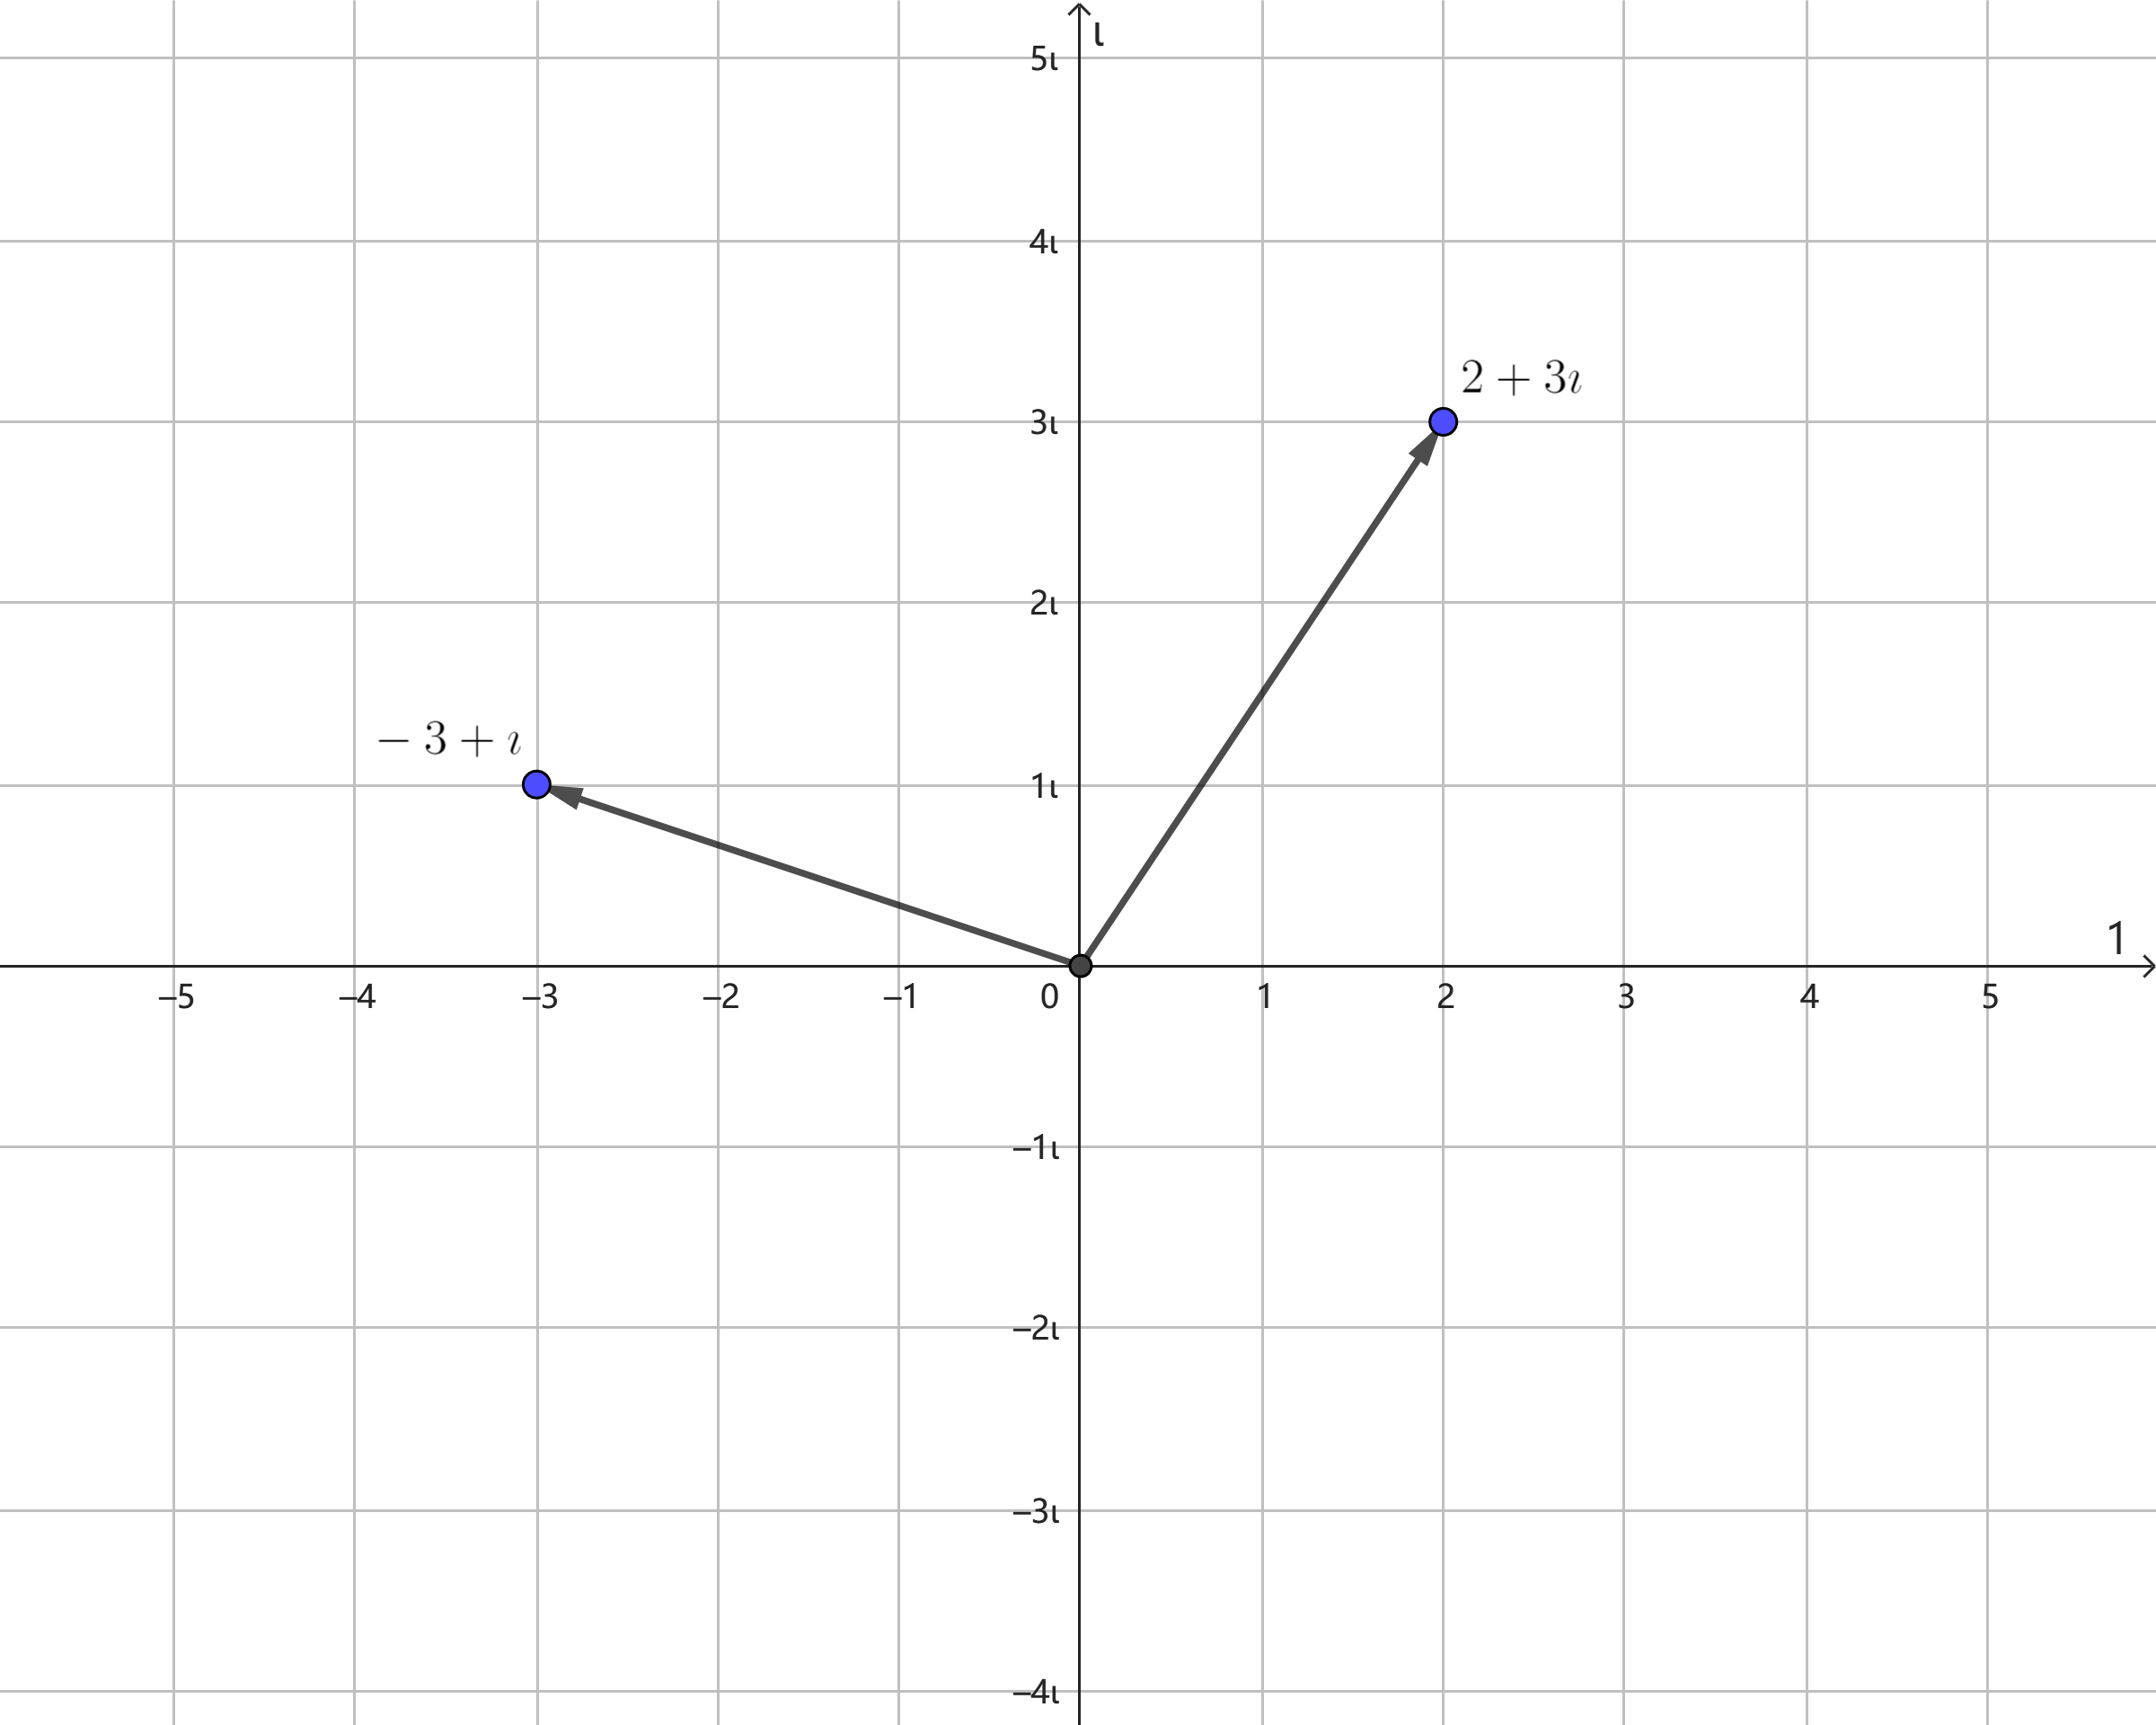
\includegraphics[width=0.8\textwidth]{tu/复平面1.png}
    \caption*{\texttt{复平面}}
\end{figure}

复平面有天然的直角坐标轴,其基向量是$1$和$\imath$。
可以说$1$和$\imath$分别是实数和虚数的单位。
复平面的原点是$0$。平面上,$\mathbb{R} = \mathbb{R}1$是一条直线,
我们可以将它看作数轴,称为复平面的\textbf{实轴}。
而直线$\mathbb{R}\imath$则称为\textbf{虚轴}。这样,复数$x+y\imath$作为复平面上的点,也叫\textbf{复向量}。
它的坐标是$(x,\,\,y)$,其中横坐标$x$称为它的\textbf{实部},纵坐标$y$称为它的\textbf{虚部}。

复数$z$的实部记为$\Re(z)$,虚部记为$\Im(z)$。两个复数相等,当且仅当实部相等、虚部相等。

将复数看作向量,它也可以定义“长度”,称为复数的\textbf{模}:
$$ |x + y\imath| = \sqrt{x^2 + y^2}.$$

我们还可以定义实轴到复数对应向量的角度,称为复数的\textbf{幅角}。

模长$r$,幅角为$\alpha$的复数,就是$r\cos{\alpha} + r\sin{\alpha}\imath$。可以用极坐标记为$(r,\,\,\alpha)$。

复数的加减法和平面向量一样。具体为:
$$ (x_1 + y_1\imath) \pm (x_2 + y_2\imath) = (x_1 \pm x_2) + (y_1 \pm y_2)\imath. $$

复数乘以实数$r$,就是分别把实部和虚部乘以$r$:
$$ r(x + y\imath) = rx + ry\imath. $$

这两个运算法则分别对应平面向量的加减法和数乘。

平面上的点不仅可以理解为向量,也可以理解为平移变换。在复平面上,点不仅可以理解为平移变换,还能理解为其他变换。

作为数域,复数比平面向量多了一个性质:复数可以作乘除法。
这等于说复平面上的两点可以相乘,得到另一个点。按照乘法规则:
$$ (x_1 + y_1\imath) \cdot (x_2 + y_2\imath) = (x_1x_2 - y_1y_2) + (x_1y_2 + x_2y_1)\imath. $$
而除法可以使用通分的技巧:
\begin{align*}
    (x_1 + y_1\imath) \div (x_2 + y_2\imath) &= \frac{(x_1 + y_1\imath)(x_2 - y_2\imath)}{(x_2 + y_2\imath)(x_2 - y_2\imath)} \\
    &= \frac{(x_1x_2 + y_1y_2) + (x_2y_1 - x_1y_2)\imath}{x_1^2 + x_2^2} \\
    &= \frac{x_1x_2 + y_1y_2}{x_2^2 + y_2^2} + \frac{x_2y_1 - x_1y_2}{x_2^2 + y_2^2}\imath
\end{align*}

根据复数乘法,我们可以有这样的结果:
\begin{align*}
     & (\cos{\alpha} + \imath\sin{\alpha}) \cdot (\cos{\beta} + \imath\sin{\beta}) \\
    =& (\cos{\alpha}\cos{\beta} - \sin{\alpha}\sin{\beta}) + (\cos{\alpha}\sin{\beta} + \cos{\beta}\sin{\alpha})\imath \\
    =& \cos{(\alpha + \beta)} + \imath\sin{(\alpha + \beta)}.
\end{align*}
直观上可以这样理解:作单位圆上与实轴夹角为$\alpha$、$\beta$的点,那么它们对应复数的乘积等于单位圆上与实轴夹角为$\alpha+\beta$的点。

\vspace{-4pt}
\begin{figure}[htp]
    \centering
\begin{tikzpicture}[>=stealth]
\draw[->](-3,0)--(3.2,0)node[below right]{$x$};
\draw[->](0,-2.5)--(0,3)node[right]{$y$};
\draw(0,0)node[below left]{$O$} circle(2);
\coordinate (Z1) at (30:2);
\coordinate (Z2) at (75:2);
\coordinate (Z3) at (45:2);
\coordinate (Z4) at (105:2);
\draw[->, thick,blue](0,0)--(Z1)node[right,blue]{$z_1$};
\draw[->, thick,blue](0,0)--(Z2)node[above right,blue]{$z_2$};
\draw[->, thick,red](0,0)--(Z3)node[above right,red]{$\displaystyle\frac{z_2}{z_1}$};
\draw[->, thick,red](0,0)--(Z4)node[above left,red]{$z_1 \cdot z_2$};
\foreach \x in {1,2,3,4}
{
    \draw[fill](Z\x) circle(2pt);
}
\draw[->,semithick,cyan] (0:0.8) arc[radius=0.8, start angle=0, end angle=30];
\draw[->,semithick,cyan] (75:0.8) arc[radius=0.8, start angle=75, end angle=105];
\draw[->,semithick,cyan] (75:0.8) arc[radius=0.8, start angle=75, end angle=45];
\end{tikzpicture}
    \caption*{\texttt{单位圆上的复数乘除法是旋转}}
\end{figure}

同样,根据复数除法,可以得到:
\begin{align*}
    & (\cos{\alpha} + \imath\sin{\alpha}) \div (\cos{\beta} + \imath\sin{\beta}) \\
   =& \frac{(\cos{\alpha}\cos{\beta} + \sin{\alpha}\sin{\beta}) + (\cos{\alpha}\sin{\beta} - \cos{\beta}\sin{\alpha})\imath}{\cos^2{\beta}+\sin^2{\beta}} \\
   =& \cos{(\alpha - \beta)} + \imath\sin{(\alpha - \beta)}.
\end{align*}
直观上,单位圆上与实轴夹角为$\alpha$、$\beta$的两点,对应复数的商等于单位圆上与实轴夹角为$\alpha-\beta$的点。

综上,乘以复数$\cos{\alpha} + \imath\sin{\alpha}$,就是在复平面上逆时针旋转$\alpha$角,而除以它,
就是顺时针旋转$\alpha$角。而乘以$r\cos{\alpha} + r\imath\sin{\alpha}$可以理解为以原点为中心放缩$r$倍,
然后逆时针旋转$\alpha$角度。

复数的加减法在复平面上有平移的效果,复数的乘除法在复平面上有旋转和放缩的效果。

最后,我们还可以对复数定义对称变换。给定复数$z = x+ y\imath$,我们说$x - y\imath$是它的\textbf{共轭复数},
简称\textbf{共轭},记作$\overline{z}$。复数的共轭,实部与它相等,虚部是它的相反数。
把复数映射到其共轭,就是关于实轴的对称变换。

复数$z$乘以它的共轭,乘积为:
$$ z \cdot \overline{z} = (x+ y\imath)(x - y\imath) = x^2 + y^2 = |z|^2. $$
复数与它的共轭的乘积总是实数,是它的模的平方。

关于复数的共轭,有这样的结论(证明见附录$A$):
\begin{tm}{\textbf{虚根成对定理}}
    如果复数$z=x+y\imath$是实系数整式$P$的根,那么它的共轭$\overline{z}=x-y\imath$也是$P$的根。
\end{tm}

共轭变换把复数映射到复数,它的出发集和到达集都是复数域。我们把出发集为复数域(也就是自变量为复数)的映射称为\textbf{复变函数}。

复变函数把复数映射到复数。如果一个函数只把复数映射到实数,也称为\textbf{复变实函数}。
反之,出发集是$\mathbb{R}$,把实数映射到复数的函数,称为\textbf{实变复函数};
只把实数映射到实数的函数,称为\textbf{实函数}。以往我们只研究实函数,称其为实变函数。
以后,我们会用实变函数泛指自变量为实数的映射\footnote{除特殊情况,实变函数不再专指实函数。}。

根据平面上对称变换和平移、旋转、放缩的关系,我们有:
\begin{align*}
    \overline{z_1 \pm z_2} &= \overline{z_1} \pm \overline{z_2} \\
    \overline{z_1 \cdot z_2} &= \overline{z_1} \cdot \overline{z_2} \\
\end{align*}

任意两个实数,可以比较大小。但两个复数一般无法比较大小。复数的模和幅角是实数,因此,我们可以比较两个复数模和幅角的大小,
但实数之间的大于小于关系,对于复数没有意义。

复数域上无法定义与复数的四则运算兼容的全序关系\footnote{全序关系:指任何两个元素都能进行比较大小。}。具体来说,想要定义复数之间的大于小于关系,使得任何两个复数之间都能比较大小,
那么这个大小关系就不能像实数的大小关系一样,和加法、乘法相容。

比如,我们可以定义两个复数的大小关系为它们模长的大小关系,模长相等则比较幅角大小。
于是有
$$1 < -2\imath, \qquad 2 < 3\imath,$$
但两者相加后:
$$ 1 + 2 = 3 > \imath = -2\imath + 3\imath.$$
不等号反向。这说明这样定义的大小关系和复数加法不相容。

复数域上没有实数那样的大小关系,因此,当我们写$a > 0$时,即是默认$a$为实数\footnote{大部分数学书籍会采用这种“暗示”方法,让叙述更简洁。}。

复数作为代数结构,比二维平直空间更丰富。因此,对不少问题来说,把实数换为复数,可以得到新的思路和结果。

\begin{et}
    \mbox{} \\
    求复数$z$使得$z^2 = 3 - 4\imath$。
\end{et}

\begin{so}
    设$z = x + y\imath$,则
    $$ z^2 = x^2 - y^2 + 2xy\imath$$
    于是可以列出方程:
    $$
    \left\{
        \begin{array}[]{rl}
            x^2 - y^2 &= 3 \\
            2xy &= -4
        \end{array}
    \right.
    $$
    从$2xy = -2$可以得出$y = -\frac{2}{x}$,代入$x^2 - y^2 = 3$得到
    $$ x^2 - \frac{4}{x^2} = 3$$
    即
    $$ x^4 - 3x^2 - 4 = 0$$
    这是关于$x^2$的一元二次方程。注意到$x^2 \geqslant 0$,所以解得:
    $$ x^2 = 4. $$
    从而有:
    $$ x = \pm 2 . $$
    代入$y = -\frac{2}{x}$,得到两组解:
    $$
    \left\{
        \begin{array}[]{rl}
            x &= 2 \\
            y &= -1,
        \end{array}
    \right.
    \qquad
    \left\{
        \begin{array}[]{rl}
            x &= -2 \\
            y &= 1
        \end{array}
    \right.
    $$ 
    即$z = 2 - \imath$或$z = -2 + \imath$。可以验证,它们的平方是$3 - 4\imath$。
    这两个复数都称为$3 - 4i$的平方根。
\end{so}

一般来说,$z^2 = a + b\imath$总有两个解。用以上方法可以求出,它们分别是:
$$
\left\{
    \begin{array}[]{rl}
        x &=\displaystyle \frac{\sqrt{2\sqrt{a^2 + b^2} + 2a}}{2} \\
        y &=\displaystyle i_b \frac{\sqrt{2\sqrt{a^2 + b^2} - 2a}}{2},
    \end{array}
\right.
\qquad
\left\{
    \begin{array}[]{rl}
        x &=\displaystyle -\frac{\sqrt{2\sqrt{a^2 + b^2} + 2a}}{2} \\
        y &=\displaystyle -i_b \frac{\sqrt{2\sqrt{a^2 + b^2} - 2a}}{2},
    \end{array}
\right.
$$ 
其中$i_b$是$b$的正负号。可以看出,两个平方根总是互为相反数,和等于$0$。复平面中,两个平方根关于原点对称。
用极坐标表示的话,复数$(r,\,\,\alpha)$的两个平方根可以表示为$\displaystyle\left(\sqrt{r},\,\,\frac{\alpha}{2}\right)$
和$\displaystyle\left(\sqrt{r},\,\,\frac{\alpha}{2}+\pi\right)$。

\begin{sk}
    \mbox{} \\
    \indent 1. 为什么说基底$(1,\,\,\imath)$构成直角坐标系?\\
    \indent 2. 复数的乘除法可以转为角度的加减法。这让你想到什么函数?它们之间有什么联系?\\
    \indent 3. 把$\imath$换成其他复数,如$\displaystyle \frac{-1+\sqrt{3}\imath}{2}$,能否构建复平面?有什么不同?
\end{sk}

\begin{xt}
    \mbox{} \\
    \indent 1. 算一算:
    $$
    \begin{array}[]{ll}
        1). \;(1.7 - \imath) + (6 - 2.9\imath)   & 2).\; (9\imath + 5.33) - (4 + 8.8\imath) \\
        3). \;(1+\imath)^2                       & 4). \;\displaystyle \frac{1 - \imath}{1 + \imath} \\
        5). \;\displaystyle (2 + i)^2 - \frac{(1 - 2i)^2 + 1}{1 + i - (3i + 1)^2 }   & 6). \;\displaystyle i^{4n+3} \\[8pt]
        7). \;\displaystyle\frac{(1 + 2\imath)^2 - (1 - \imath)^2}{(3 + 2\imath)^2 + \imath + 2} & 8). \;\displaystyle\frac{(2 + \imath)^2 + (1 - \imath)^2 - \imath}{1 + \imath + (2\imath - 1)^2} \\
    \end{array}
    $$
    \indent 2. 算一算:
    $$
    \begin{array}[]{ll}
        1). \;|2 - 2.9\imath|^2   & 2).\; |1 - 2a + (a - 1)\imath|^2 \\[4pt]
        3). \;|(x + y) - (x - y)\imath|^2   & 4).\;\displaystyle\left|\frac{1 - \imath}{1 + \imath} \right|\\
    \end{array}
    $$
    \indent 3. 验证:复数满足加法、乘法的交换律和结合律,以及乘法对加法的分配律。\\
    \indent 4. 验证以下说法:\\
    \indent 4.1. 复数$z$是实数,当且仅当它等于它的实部;复数$z$是虚数,当且仅当它等于它的虚部。\\
    \indent 4.2. 复数$z$的实部是$iz$的虚部,虚部是$-iz$的实部。\\
    \indent 4.3. 复数$z$的共轭等于自己,当且仅当它是实数。\\
    \indent 4.4. 复数$z$的实部等于$\overline{z}$的实部,虚部等于$\overline{z}$的虚部的相反数。\\
    \indent 4.5. 复数$z$的模等于$\overline{z}$的模。\\
    \indent 5. 设非零复数$z = r(\cos{\alpha} + \imath\sin{\alpha})$。\\
    \indent 5.1. 证明:对任意自然数$n$,$z^n = r^n(\cos{(n\alpha)} + \imath\sin{(n\alpha)})$。 \\
    \indent 5.2. 证明:对任意正整数$n$,有$n$个复数$x$满足$x^n = z$。写出这$n$个复数。它们在复平面上有何关系?\\
    \indent 5.3. 证明:对任意有理数$q$,$r^q(\cos{(q\alpha)} + \imath\sin{(q\alpha)}) = z^q$。 \\
    \indent 6. 证明:复数的共轭满足:\\
    \indent 6.1. $ \overline{\overline{z}} = z.$ \\
    \indent 6.2. $ \overline{z_1 \pm z_2} = \overline{z_1}\pm \overline{z_2}.$ \\
    \indent 6.3. $ z + \overline{z} = 2\Re(z), \quad z - \overline{z} = 2\Im(z).$\\
    \indent 6.4. $\displaystyle\overline{z_1 \cdot z_2} = \overline{z_1}\cdot \overline{z_2}, \quad \overline{\left(\frac{z_1}{z_2}\right)} = \frac{\overline{z_1}}{\overline{z_2}}.$ \\
    \indent 6.5. $ z\cdot \overline{z} = |z|^2 = |\overline{z}|^2.$ \\
    \indent 7. 证明:对任意复数$z$、$w$,有\\
    \indent 7.1. $ |z + w| \leqslant |z| + |w|.$ \\
    \indent 7.2. $ |z + w|^2 + |z - w|^2 \leqslant 2(|z|^2 + |w|^2).$ \\
    \indent 7.3. $ \displaystyle|zw| = |z|\cdot |w|, \quad \left|\frac{z}{w}\right| = \frac{|z|}{|w|}. $
\end{xt}

\section{单位根}

让我们来看这样的方程:
$$ x^n = 1.$$
其中$n$是正整数。根据整数有根定理的推论,它在$\mathbb{C}$中有$n$个解。我们可以把这$n$个解都找出来。它们分别是:
\begin{align*}
    \begin{cases}
        z_1 &= \cos{\left(\frac{2\pi}{n}\right)} + \imath \sin{\left(\frac{2\pi}{n}\right)} \\
        z_2 &= \cos{\left(\frac{4\pi}{n}\right)} + \imath \sin{\left(\frac{4\pi}{n}\right)} \\
        & \quad\quad \vdots \\[-4pt]
        z_k &= \cos{\left(\frac{2k\pi}{n}\right)} + \imath \sin{\left(\frac{2k\pi}{n}\right)} \\
        & \quad\quad \vdots \\[-4pt]
        z_n &= \cos{\left(\frac{2n\pi}{n}\right)} + \imath \sin{\left(\frac{2n\pi}{n}\right)} = 1. \\
    \end{cases}
\end{align*}

在复平面上画出这$n$个复数,可以发现,它们都在单位圆上。
我们把这$n$个解称为$\boldsymbol{n}$\textbf{次单位根}。

单位根都在单位圆上,它们的模都是$1$。不仅如此,$n$个$n$次单位根$z_1,z_2,\cdots, z_n$都可以看作$z_1$的乘方,分别是$z_1$的$1$次方、$2$次方、……$n$次方。
因此,我们也会把$n$次单位根记为$\omega_n^1, \omega_n^2, \cdots, \omega_n^n$或$\omega_n^0, \omega_n^1, \omega_n^2, \cdots, \omega_n^{n-1}$,
其中$\omega_n$就是$z_1$,也叫做$\boldsymbol{n}$\textbf{次基本单位根}。

\vspace{-4pt}
\begin{figure}[htp]
    \centering
\begin{tikzpicture}[>=stealth]
\draw[->](-2.5,0)--(2.7,0)node[below right]{$x$};
\draw[->](0,-2)--(0,2.7)node[right]{$y$};
\draw(0,0)node[below left]{$O$} circle(1.5);
\coordinate (Z1) at (0:1.5);
\coordinate (Z2) at (36*2:1.5);
\coordinate (Z3) at (36*4:1.5);
\coordinate (Z4) at (36*6:1.5);
\coordinate (Z5) at (36*8:1.5);
\draw[->, thick,blue](0,0)--(Z1)node[above right,blue]{$z_5=1$};
\draw[->, thick,blue](0,0)--(Z2)node[above,blue]{$z_1$};
\draw[->, thick,blue](0,0)--(Z3)node[above left,blue]{$z_2$};
\draw[->, thick,blue](0,0)--(Z4)node[below left,blue]{$z_3$};
\draw[->, thick,blue](0,0)--(Z5)node[below right,blue]{$z_4$};
\foreach \x in {1,2,3,4,5}
{
    \draw[fill](Z\x) circle(1.5pt);
}
\end{tikzpicture}
    \caption*{$n$\texttt{次单位根“等角分布”在单位圆上(}$n=5$\texttt{)}}
\end{figure}

直观上,这说明单位根的幅角都是$z_1$的整数倍。换句话说,这些复数在单位圆上“等角分布”,是单位向量$(0,\;1)$逆时针不断旋转相同的角度次第形成的。
相邻的两个单位根$z_i$和$z_{i+1}$的夹角总是$\displaystyle \frac{2\pi}{n}$。

\vspace{-4pt}
\begin{minipage}{.45\textwidth}
    \centering
    \begin{tikzpicture}[>=stealth]
    \draw[->](-2.5,0)--(2.7,0)node[right]{$x$};
    \draw[->](0,-2)--(0,2.7)node[right]{$y$};
    \draw(0,0)node[below left]{$O$} circle(1.5);
    \draw[thick,blue](1.5,0)node[above right]{$z_3$}--(120:1.5)node[above]{$z_1$}--(240:1.5)node[below]{$z_2$}--cycle;
    
    \end{tikzpicture}
    \end{minipage}\hfill
    \begin{minipage}{.45\textwidth}
    \centering
    \begin{tikzpicture}[>=stealth]
        \draw[->](-2.5,0)--(2.7,0)node[right]{$x$};
        \draw[->](0,-2)--(0,2.7)node[right]{$y$};
        \draw(0,0)node[below left]{$O$} circle(1.5);
    \draw[thick,blue](1.5,0)node[above right]{$z_4$}--(0,1.5)node[above right]{$z_1$}--(-1.5,0)node[above left]{$z_2$}--(0,-1.5)node[below left]{$z_3$}--cycle;
    
    \end{tikzpicture}
    \end{minipage}

$n\geqslant 3$时,我们可以说$n$次单位根是单位圆的内接正$n$边形的顶点,其中固定的顶点是$(0,\;1)$。
这个正$n$边形关于复平面的$x$轴对称,因此,单位根之间也有对称的关系。根据虚根成对定理,单位根的共轭还是单位根。
比如,$z_1$的共轭就是$z_{n-1}$,$z_2$的共轭就是$z_{n-2}$,等等。一般来说,$z_k$的共轭是$z_{n-k}$。

如果$n$是偶数,那么$-1$也是单位根。这时,所有单位根为顶点的单位圆内接正$n$边形不仅关于复平面的$x$轴对称,还关于$y$轴对称。

\begin{figure}[h]
    \vspace{-8pt}
    \centering
\begin{tikzpicture}[>=stealth]
    \draw[->](-2.5,0)--(2.7,0)node[below]{$x$};
    \draw[->](0,-2)--(0,2.5)node[right]{$y$};
    \draw(0,0)node[below left]{$O$} circle(1.5);
\foreach \x in {0,1,2,...,4}
{
    \draw[fill,blue](\x*72:1.5) circle(1.5pt);
}
\node at (1.4,-0.05)[above right,blue]{$z_{5} = \omega_{5}^{5} = 1$};
\node at (78:1.5)[above right,blue]{$z_1 = \omega_{5}$};
\node at (150:1.5)[above left,blue]{$z_2 = \omega_{5}^{2}$};
\node at (200:1.2)[below left,blue]{$\begin{array}{r}
    z_3 = \omega_{5}^{3} \\[-4pt] = \overline{z_2}\phantom{\,}
\end{array}$};
\node at (-78:1.4)[below right,blue]{$z_{4} = \omega_{5}^{4} = \overline{z_1}$};
\end{tikzpicture}
\begin{tikzpicture}[>=stealth]
    \draw[->](-2.5,0)--(2.7,0)node[below]{$x$};
    \draw[->](0,-2)--(0,2.5)node[right]{$y$};
    \draw(0,0)node[below left]{$O$} circle(1.5);
\foreach \x in {0,1,2,...,11}
{
    \draw[fill,blue](\x*30:1.5) circle(1.5pt);
}
\node at (1.4,-0.05)[above right,blue]{$z_{12} = \omega_{12}^{12} = 1$};
\node at (30:1.35)[above right,blue]{$z_1 = \omega_{12}$};
\node at (65:1.4)[above right,blue]{$z_2 = \omega_{12}^{2}$};
\node at (-25:1.4)[below right,blue]{$z_{11} = \omega_{12}^{11} = \overline{z_1}$};
\end{tikzpicture}
\caption*{$5$\texttt{次单位根(左)和}$12$\texttt{次单位根(右)在复平面上的分布}}
\end{figure}

我们可以用单位根来表示一般复数开方的结果。比如,设$r$为正实数,那么$x^n = r$的解为:
$$ \forall k\in  [1..n], \quad z_k = \sqrt[n]{r}\left(\cos{\frac{2k\pi}{n}} + \imath \sin{\frac{2k\pi}{n}}\right) = \sqrt[n]{r}\omega_n^k. $$
我们把这$n$个解都称为$a$的$n$次方根。

同理,如果复数$z$可以表示为$z = r(\cos{\alpha} + \imath \sin{\alpha})$,那么$x^n = z$的解为:
$$ \forall k\in  [1..n], \; z_k = \sqrt[n]{r}\left(\cos{\frac{2k\pi + \alpha}{n}} + \imath \sin{\frac{2k\pi + \alpha}{n}}\right) = \sqrt[n]{r}\left(\cos{\frac{\alpha}{n}} + \imath \sin{\frac{\alpha}{n}}\right)\omega_n^k. $$
我们把这$n$个解都称为$z$的$n$次方根。

\begin{sk}
    \mbox{} \\
    \indent 1. 比较$n$次单位根和$n$次同余系,它们有什么共同点?\\
    \indent 2. 考虑复数数列$\displaystyle\left\{\cos{\frac{k\sqrt{2}\pi}{n}} + \imath \sin{\frac{k\sqrt{2}\pi}{n}} \right\}_{k\in\mathbb{N}}$,它在复平面上对应的点有什么特征,有什么规律?
\end{sk}

\begin{xt}
    \mbox{} \\
    \indent 1. 写出$3$次单位根和$4$次单位根。 \\
    \indent 2. 验证以下结论:\\
    \indent 2.1. 任意$n$次单位根的任意乘方仍然是$n$次单位根。\\
    \indent 2.2. 如果$m$整除$n$,那么$m$次单位根也是$n$次单位根。\\
    \indent 2.3. 如果$k$与$n$互素,那么$n$次单位根可以表示为$\omega_n^k, \omega_n^{2k}, \cdots , \omega_n^{nk}$,不重复也不遗漏。\\
    \indent 2.4. $ \forall n\in\mathbb{Z}^+, \quad \omega_n + \omega_n^2 + \cdots + \omega_n^n = 0. $\\
    \indent 3. 在$\mathbb{C}$中解以下方程:
    \begin{align*}
        1)\;& x^5 + 1 = 0,  & 2)\;& x^{12} + 63x^6 - 64 = 0 \\
        3)\;& x^3 = 1 - \sqrt{3}\imath,  & 4)\;& 4x^8 - 2x^4 + 1 = 0 
    \end{align*}
    \indent 4. 考虑四个两两不同的复数:$z_1,z_2,z_3,z_4$。\\
    \indent 4.1. 证明:两个非零复数之比为实数,当且仅当它们幅角相差$\pi$的倍数。\\
    \indent 4.2. 将$z_1,z_2,z_3,z_4$在复平面上的点记为$A,B,C,D$,解释以下复数的直观意义:
    $$ \frac{z_1 - z_2}{z_3 - z_2}, \quad \frac{z_4 - z_2}{z_4 - z_3}  $$
    \indent 4.3. 证明:以下条件成立,当且仅当$A,B,C,D$四点共线或共圆。
    $$ \frac{z_1 - z_3}{z_2 - z_3} = r \frac{z_1 - z_4}{z_2 - z_4}, \quad r\in \mathbb{R}. $$
    \indent 并分别说明$r$为正数、负数时的情况。

\end{xt}

\chapter{平面的曲线}

曲线是十分常见的平面形。我们学习过的曲线有圆和经典函数的曲线。

微变和积合的知识,让我们有了不少研究曲线的新工具。比如,我们可以用微变研究函数曲线的增减和凹凸性,
用微变展开研究函数曲线局部的形状,等等。

下面我们会引进一些常见的经典曲线,并应用微变和积合的知识,研究曲线的性质。

\section{描述曲线}

我们已经学习过实函数的曲线。
已知定义在区间$I$上的连续函数$f$,集合
$$ \{(x,\,\,f(x)) ,\ | \, x\in I\}$$
就是函数的曲线。

实变函数曲线的特征是:用平行于$y$轴的直线截函数曲线,只有一个交点。
这是因为按照映射的定义,映射总把自变量映射到一个值上。实函数的出发集和到达集都是实数。
因此,实函数的一个自变量总对应一个实数,平行于$y$轴的直线$x = a$永远只对应一个实数:$f(a)$。

一般来说,曲线是平面的一种子集。因此,用方程描述曲线,是常见的方法。曲线就对应方程的解集。

我们已经见过,圆的方程是:
$$ x^2 + y^2 = r^2 $$
这个方程对应平面的子集:
$$ \{(x,\,\,y ) \, | \, x^2 + y^2 = r^2 \}.$$

同理,很多曲线可以用关于平面点的方程来刻画。

另一种刻画曲线的方法,是把曲线的点表示成另一个变量的映射。比如,圆可以表示为:
\begin{align*}
    f: [0;2\pi] &\rightarrow \mathbb{R}^2 \\
    t\quad &\mapsto\left\{
        \begin{array}[]{rl}
            x(t) &= r\cos{t} \\
            y(t) &= r\sin{t} \\
        \end{array}
    \right.
\end{align*}

其中变量$t$称为\textbf{参变量},而以上的映射称为曲线的\textbf{参变映射},这样刻画的曲线称为\textbf{参变曲线}。
参变映射把参变量$t$映射到点$(x(t),\,\, y(t))$。参变映射通常是连续函数。如果参变映射是单射(不会两次经过同一个点\footnote{首尾两端点例外。}),
就说参变曲线是\textbf{简单曲线}。如果首尾重合,就说它是\textbf{闭合曲线}。比如,上述圆的参变映射$f$满足:
$$ f(0) =  (1, \,\,0) = f(2\pi). $$
首尾重合,因此是闭合曲线。

参变曲线和方程刻画曲线的区别在于多了参变量。在很多实际问题中,参变量有其实际含义。
比如很多运动轨迹问题中,用时间$t$作为参变量。

\begin{sk}
    \mbox{} \\
    \indent 1. 如何用参变映射描述实函数的曲线?\\
    \indent 2. 如何用方程刻画参变曲线?反之,如何用参变映射刻画以方程表示的曲线?
\end{sk}

\section{二次曲线}

首先来看整式方程定义的曲线。一次方程描述的总是直线。因此,我们可以说二次方程对应的曲线是整式方程中“最简单的”。

一般来说,二次曲线是以下方程定义的曲线:
$$ Ax^2 + Bxy + Cy^2 + Dx + Ey + F = 0.$$
其中$A$、$B$、$C$不同时为零。

我们知道,如果$B = 0$,而$A = C$不为零,那么定义的曲线是圆。
再来看几个典型的例子。

首先假设$B = 0$。

% 椭圆例图
\begin{wrapfigure}[5]{r}{0.32\textwidth} %this figure will be at the right
    \vspace{-30pt}
    \flushright
    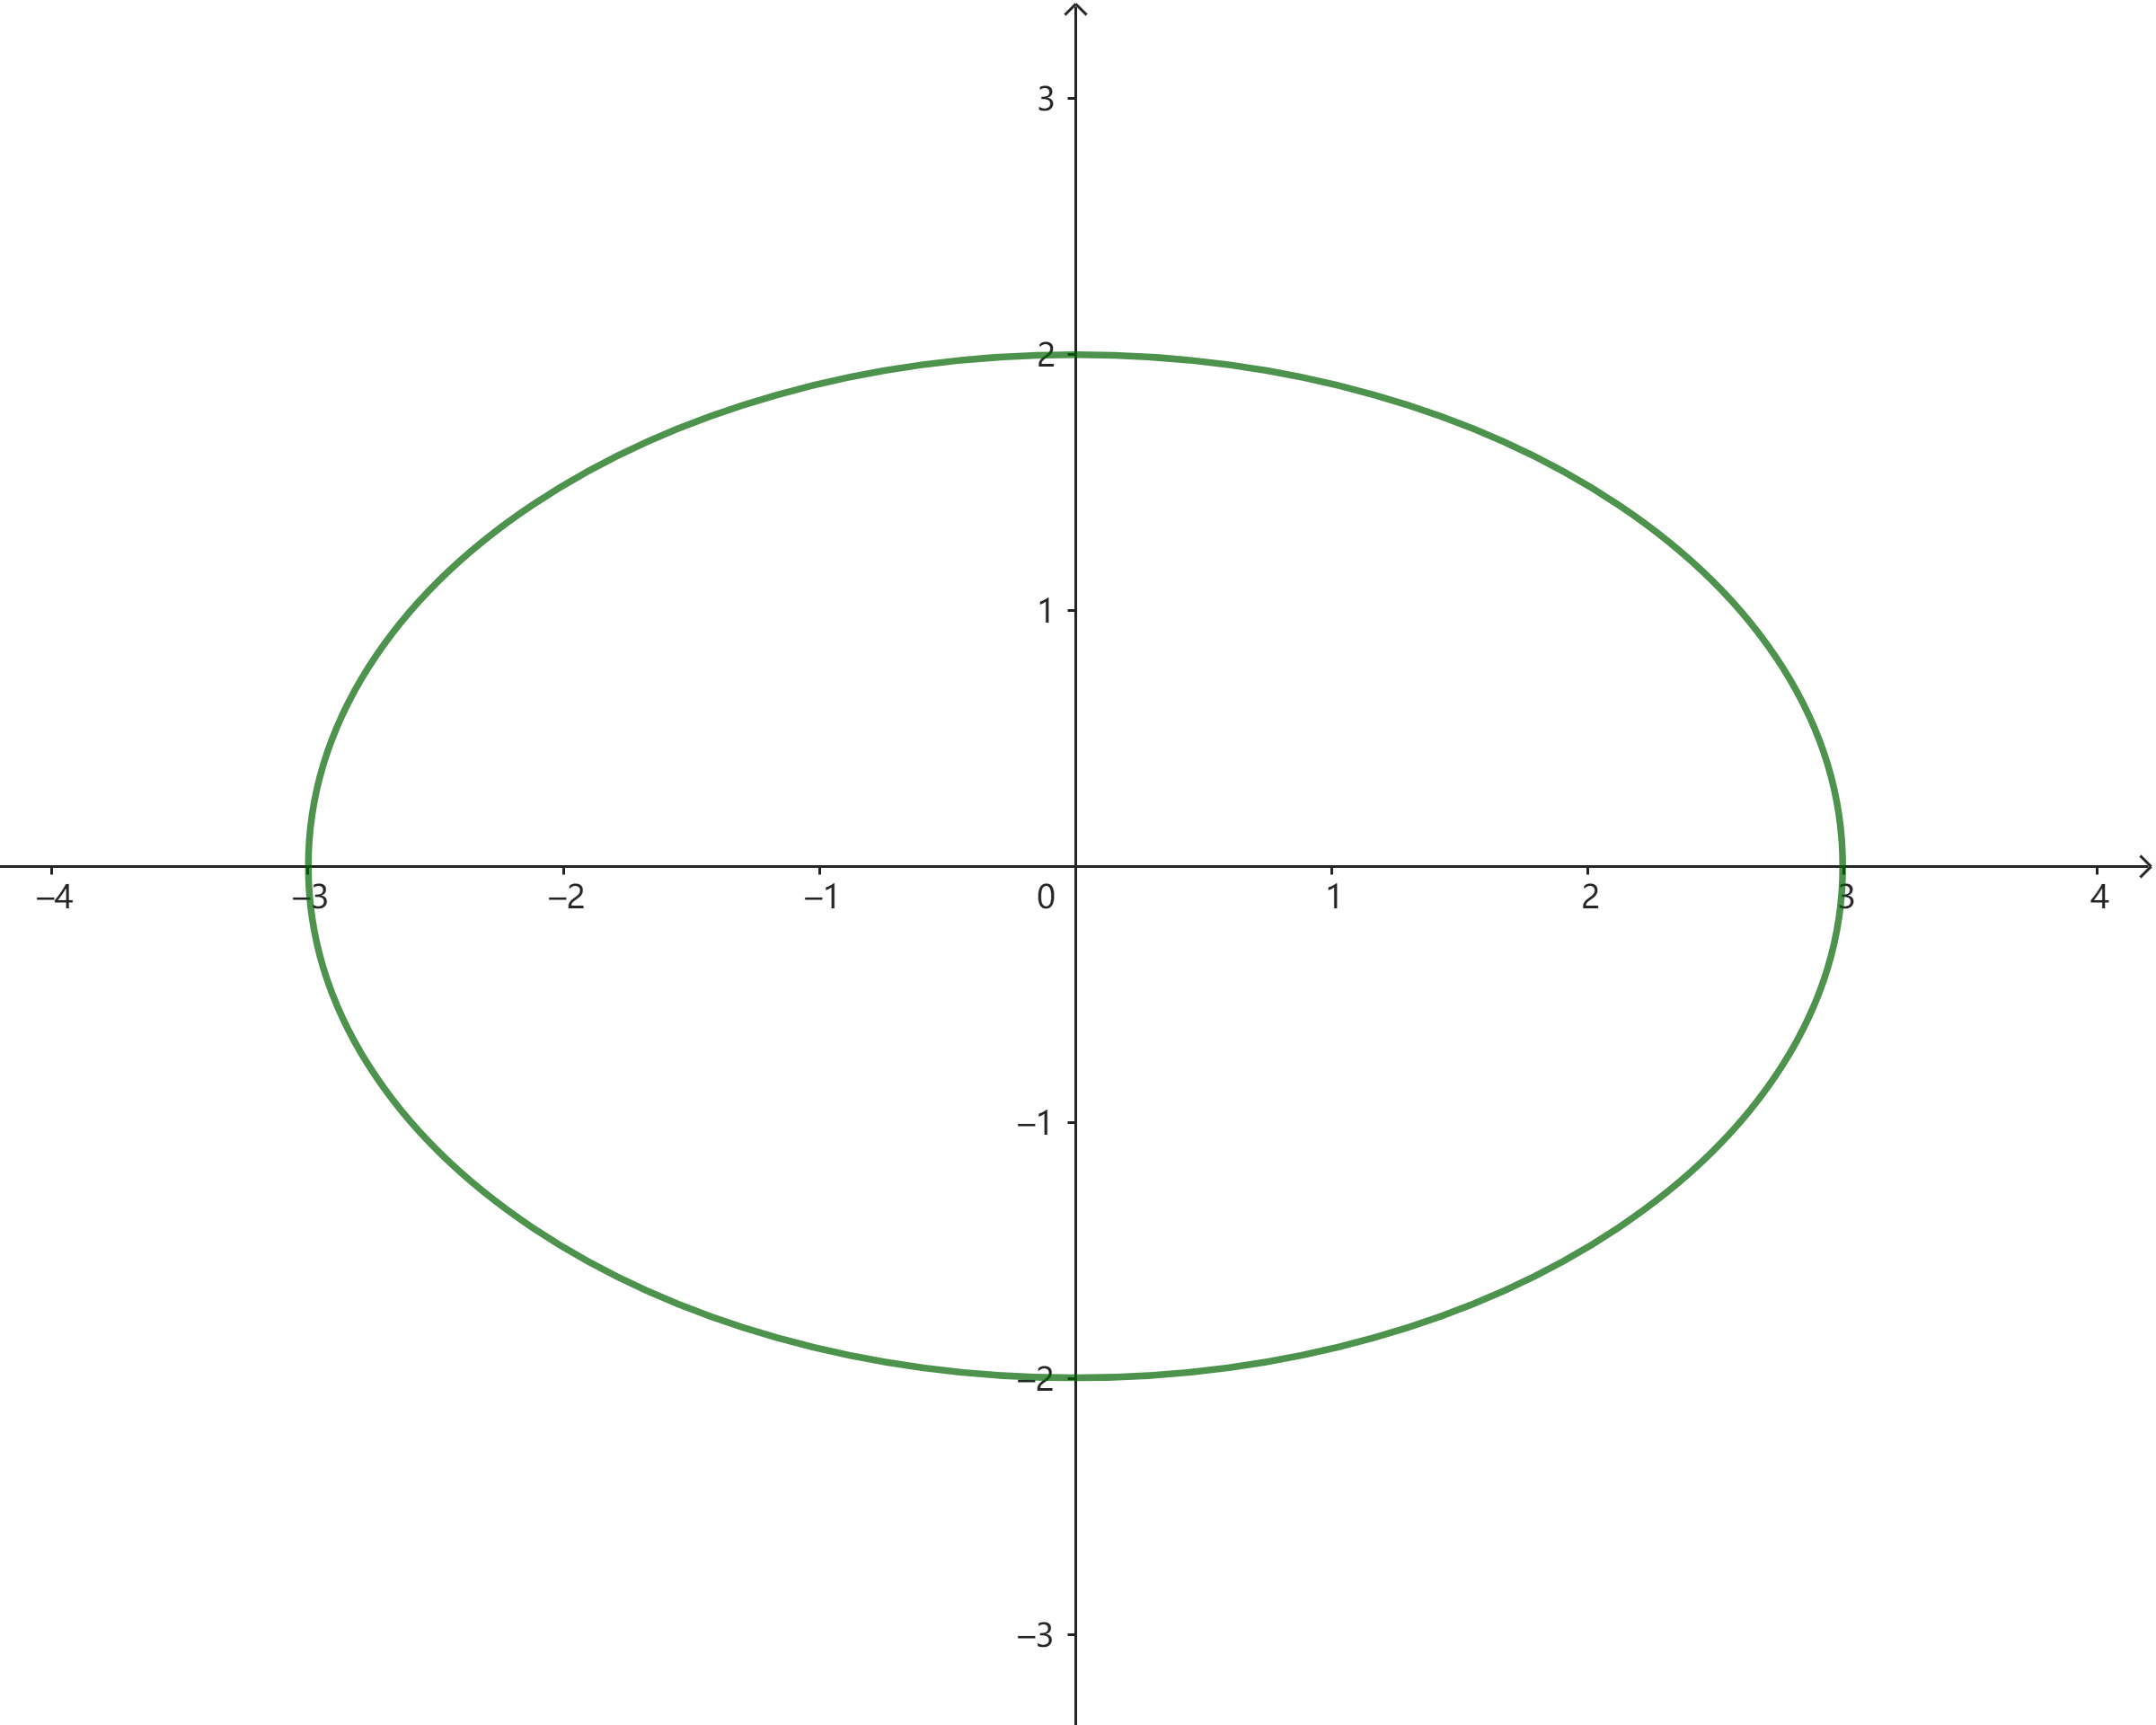
\includegraphics[width=0.3\textwidth]{tu/椭圆1.png}
\end{wrapfigure}

如果$AC > 0$,可以画出曲线如图。这样的曲线称为椭圆。典型的椭圆方程可以写为:
$$ \frac{x^2}{a^2} + \frac{y^2}{b^2} = 1 $$
其中$a,b>0$。

从这个方程来看,椭圆可以理解为圆经过$x$轴方向(或$y$轴方向)放缩得到。椭圆的曲线是闭合曲线。
椭圆上的点$(x,\,\,y)$总满足
$$ -a \leqslant x \leqslant a, \quad -b \leqslant y \leqslant b$$
这说明椭圆曲线是有界的。

% 双曲线例图(渐近线)
\begin{wrapfigure}[5]{r}{0.32\textwidth} %this figure will be at the right
    \vspace{-12pt}
    \flushright
    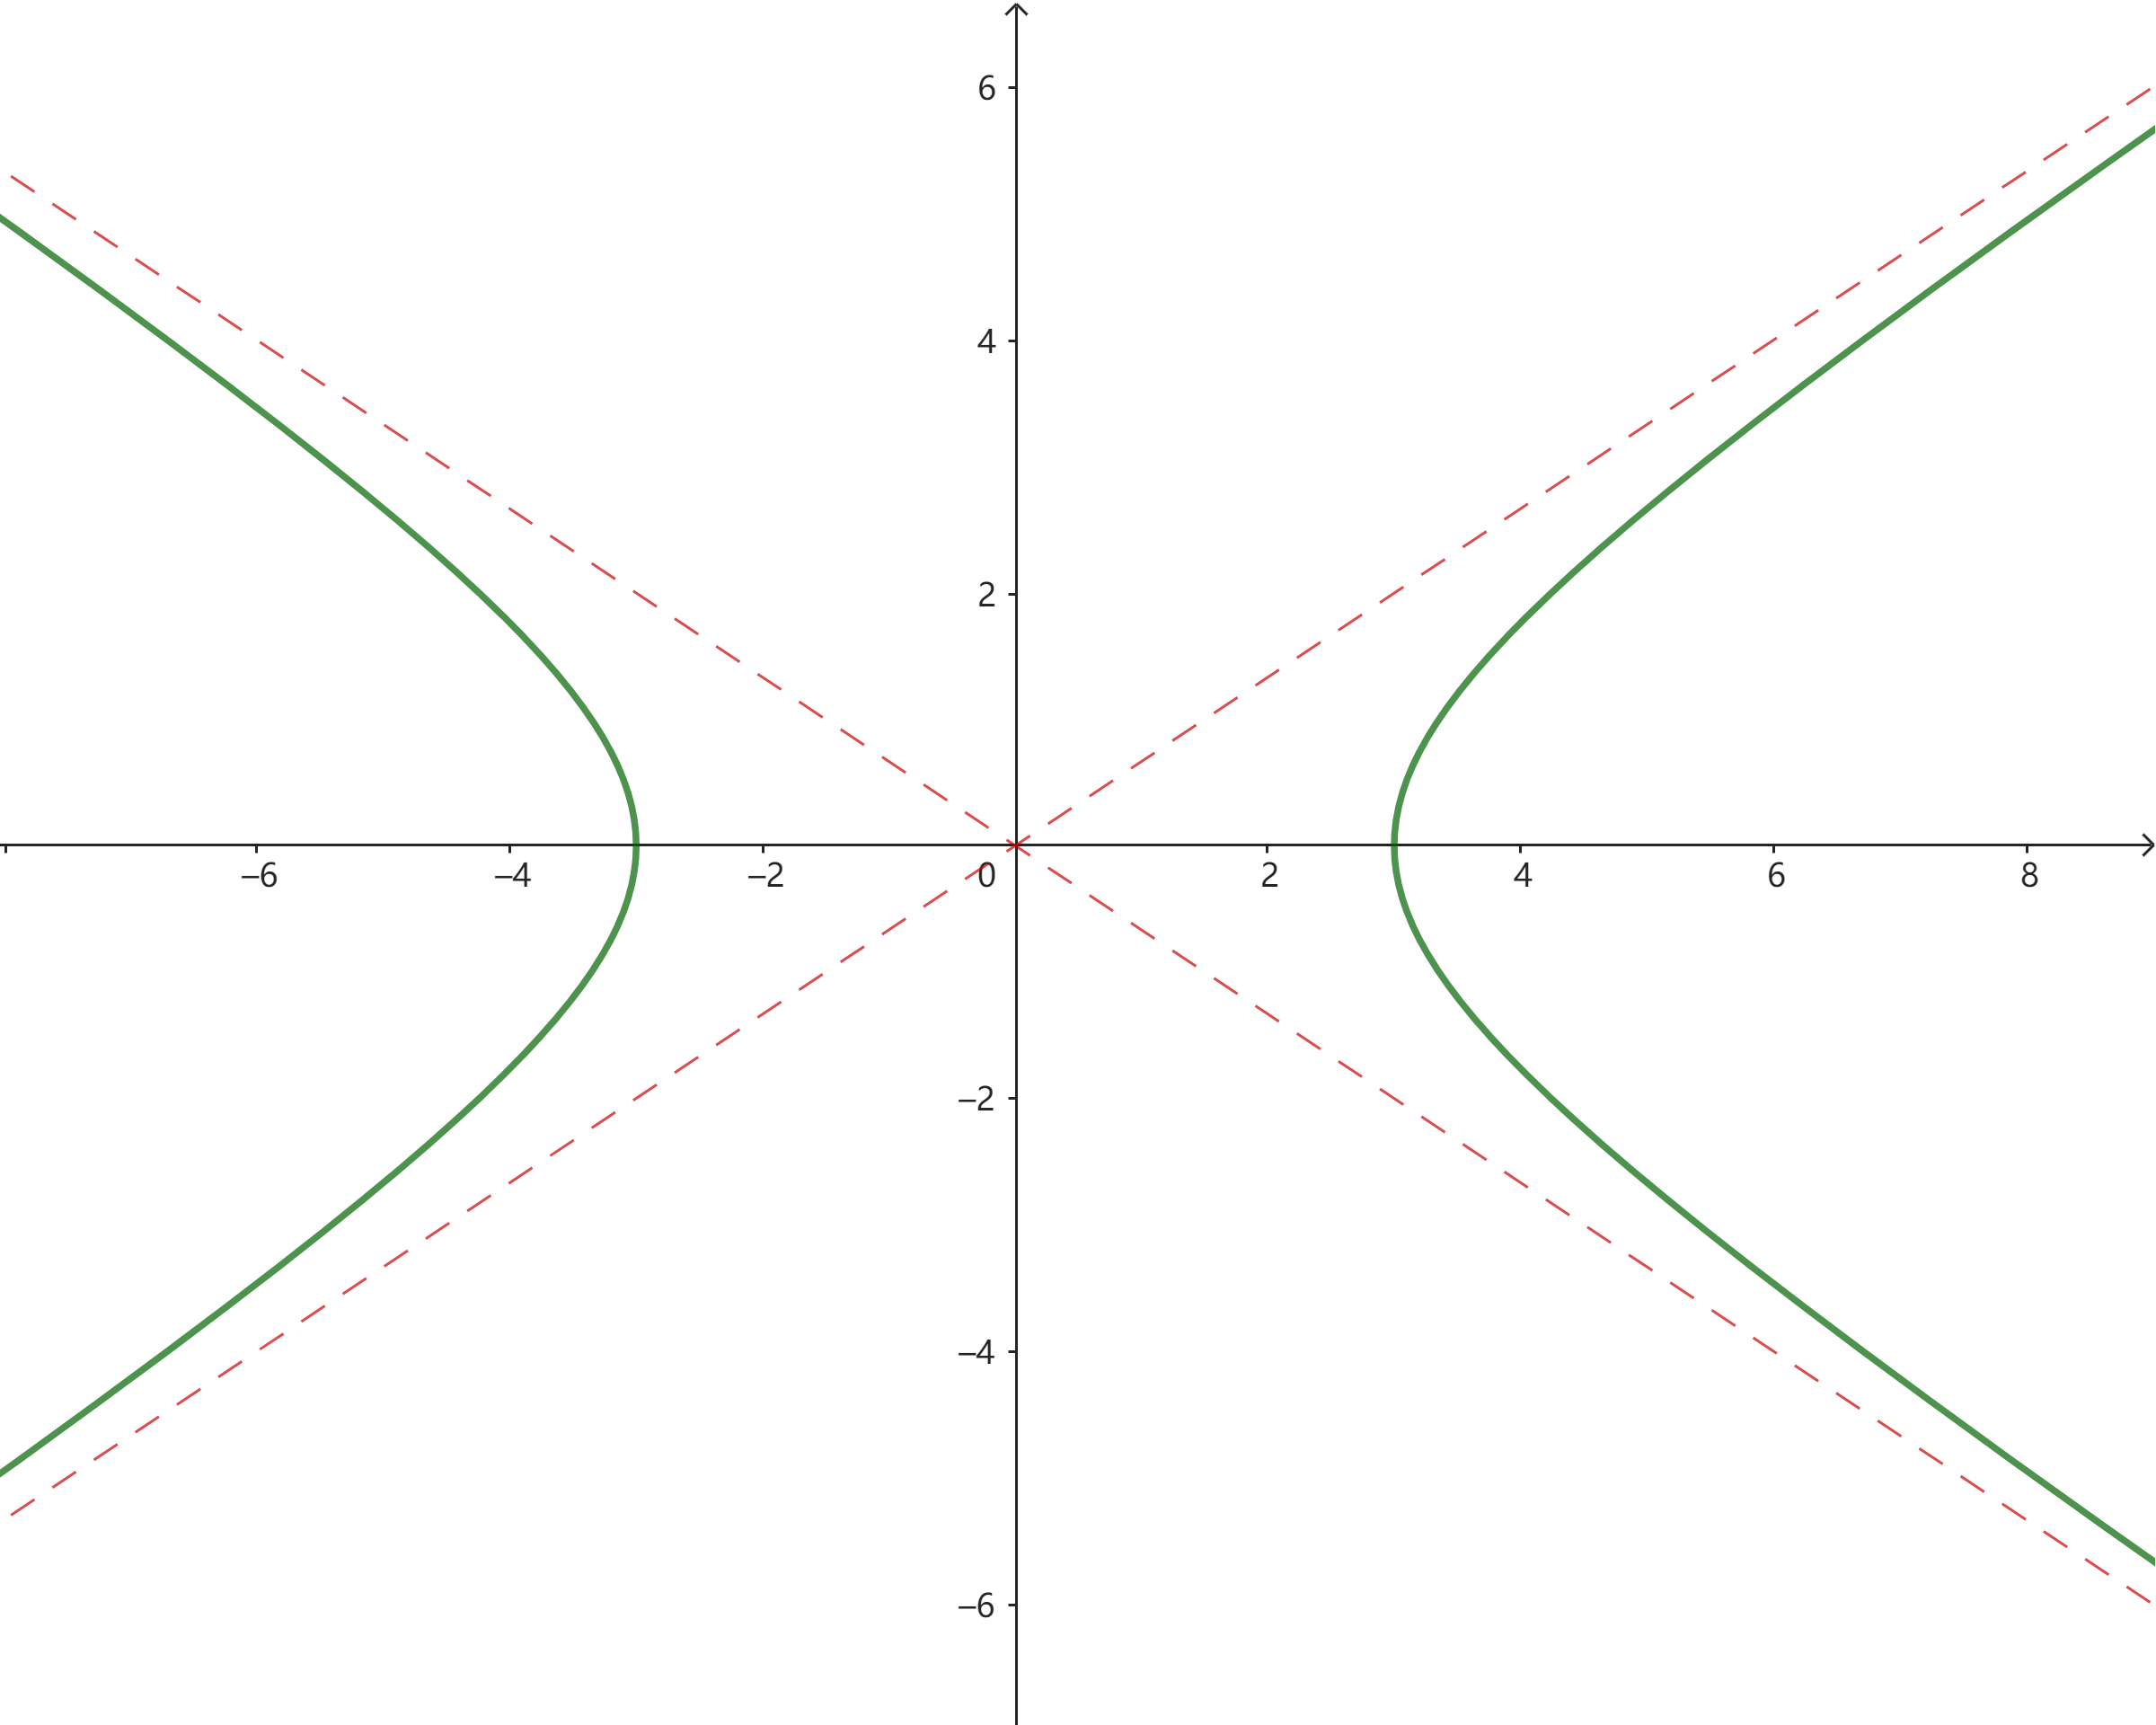
\includegraphics[width=0.3\textwidth]{tu/双曲线1.png}
\end{wrapfigure}

如果$B = 0$,$AC < 0$,可以画出曲线如图。这样的曲线称为双曲线。典型的双曲线方程可以写为:
$$ \frac{x^2}{a^2} - \frac{y^2}{b^2} = 1 \quad \mbox{(如右图)}$$
或
$$ - \frac{x^2}{a^2} + \frac{y^2}{b^2} = 1  \quad \mbox{(如左下图)} \qquad  \qquad  \qquad  \qquad \;\: \quad \phantom{123}$$
其中$a,b>0$。

\begin{wrapfigure}[5]{l}{0.32\textwidth} 
    \vspace{-28pt}
    \flushright
    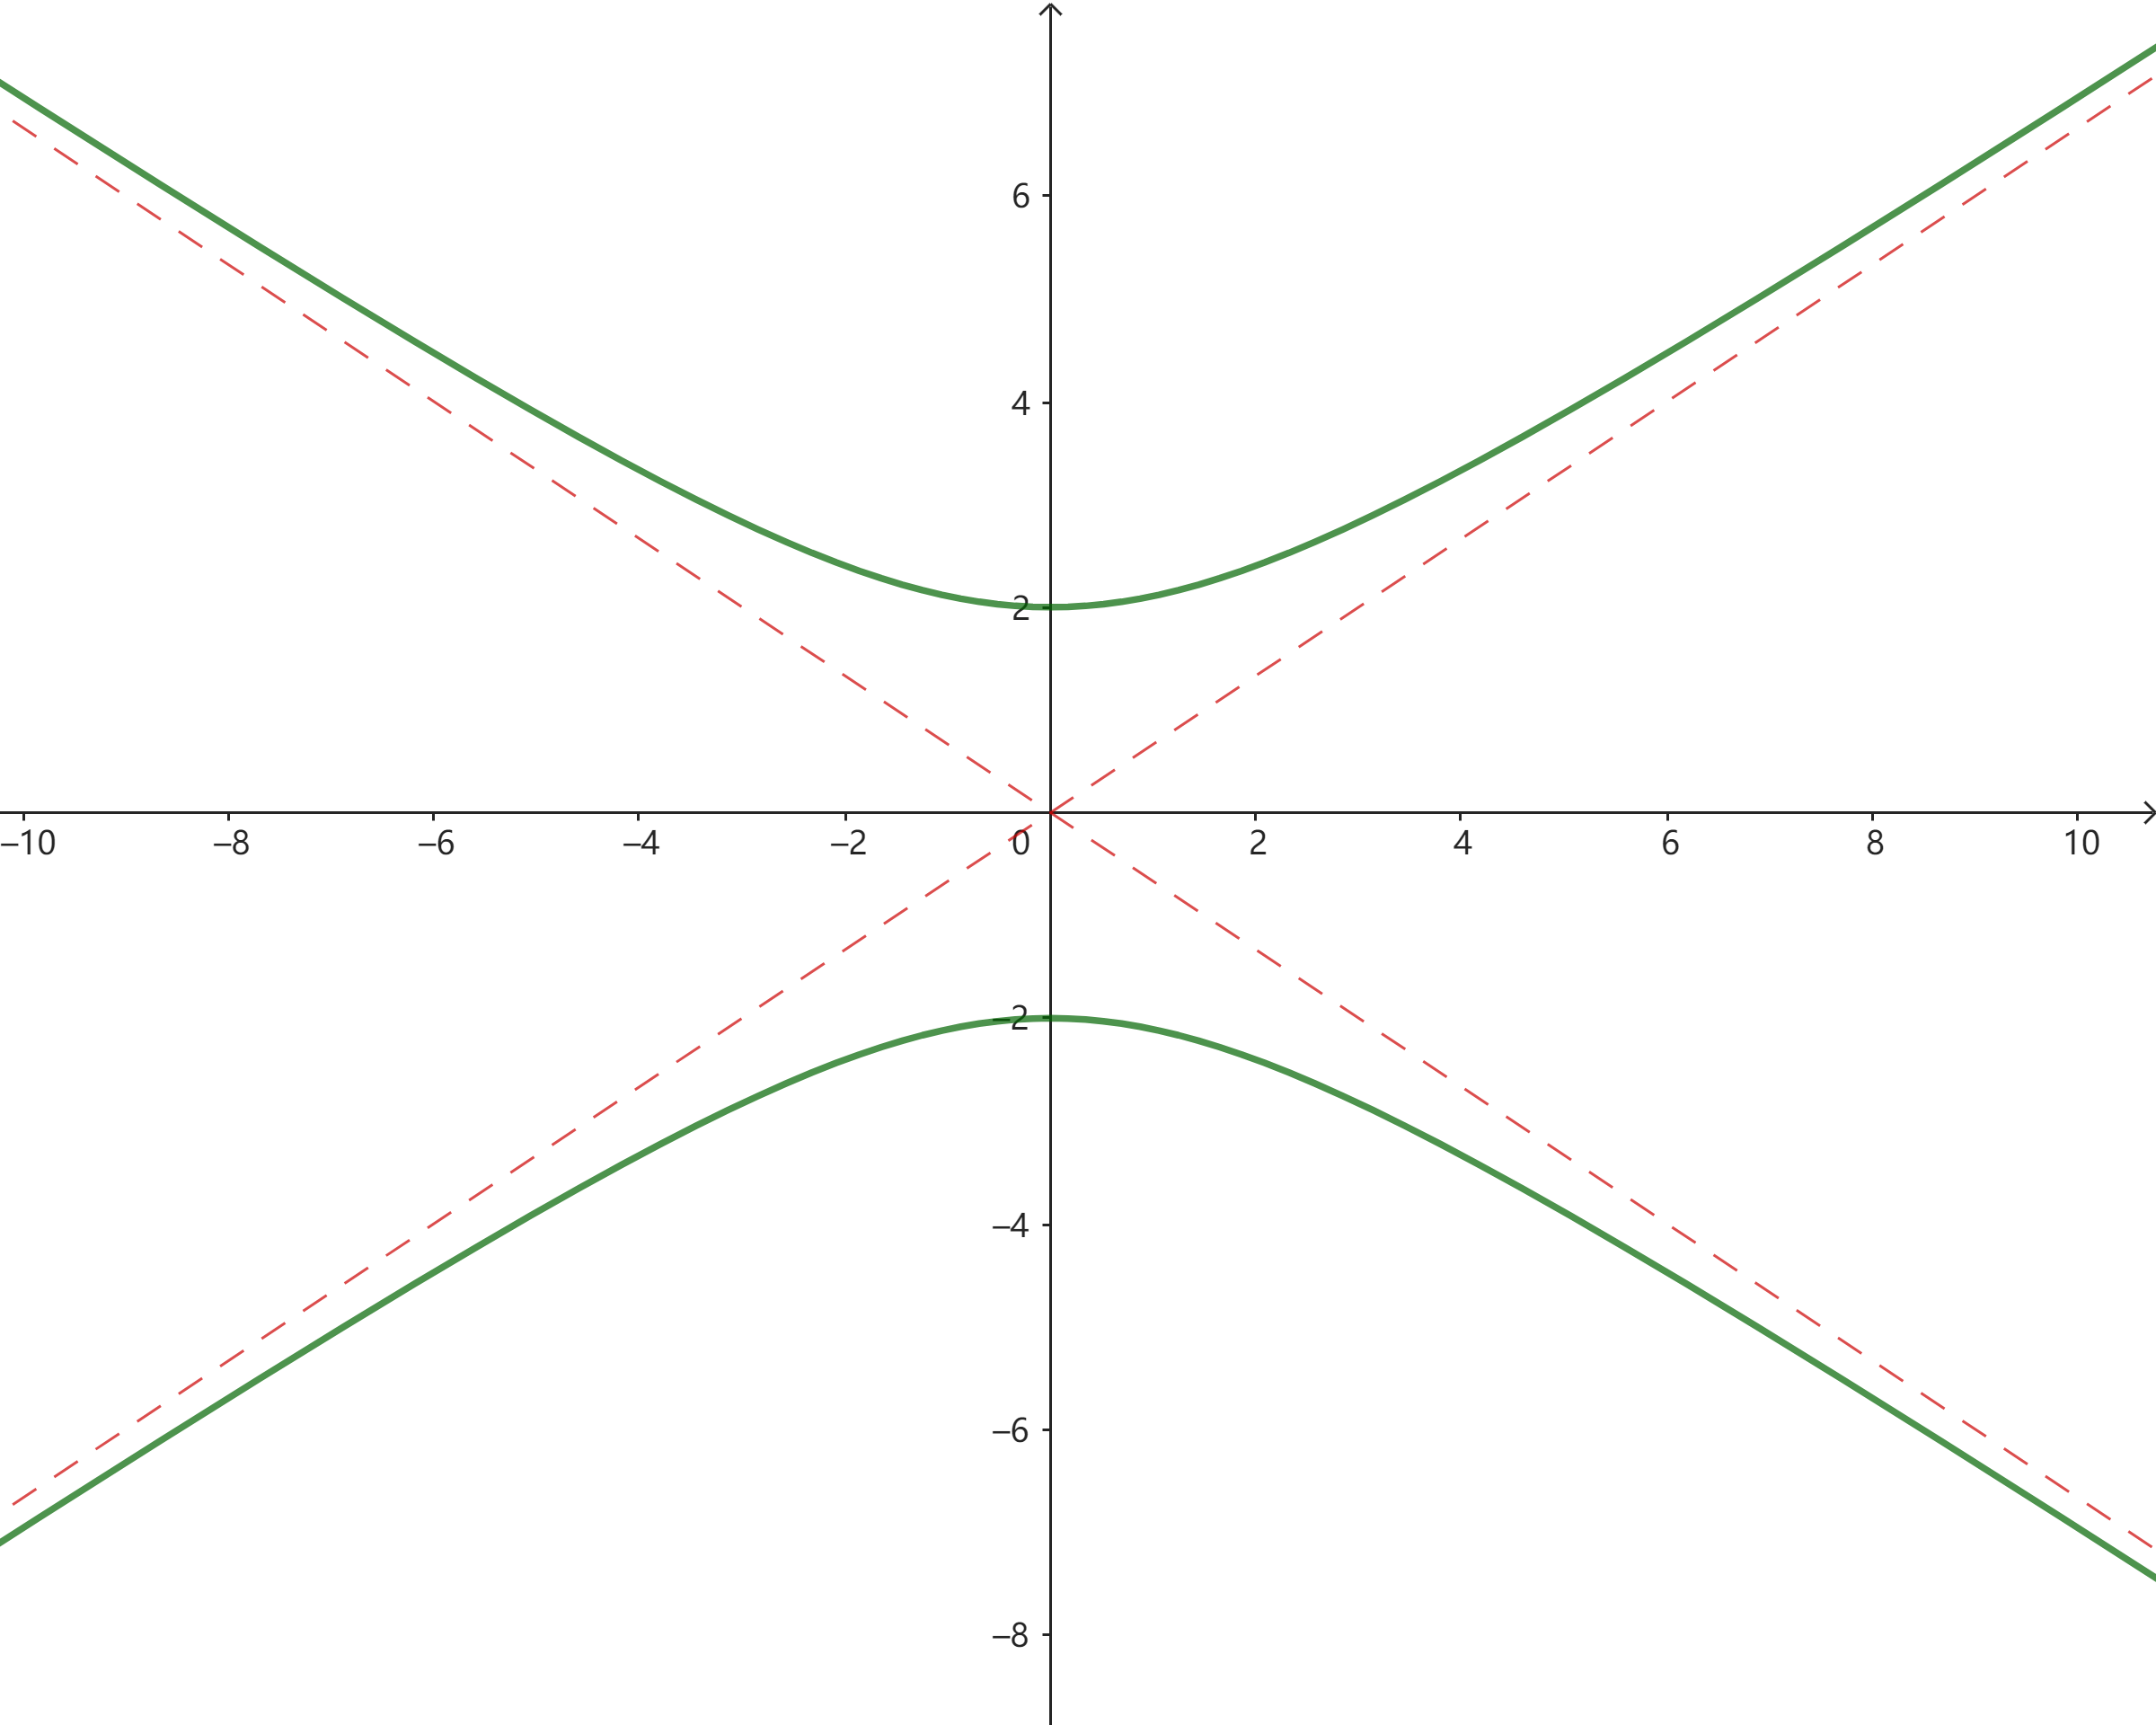
\includegraphics[width=0.3\textwidth]{tu/双曲线2.png}
\end{wrapfigure}

可以看到,双曲线由两个不相连的分支构成,一般按位置称为上下支或左右支。曲线不是闭合的,而是无界的,
关于$x$轴和$y$轴对称。
随着$x$趋于无穷,$y$也趋于无穷,反之亦然。而由于
$$ \phantom{123455}\qquad \qquad \qquad \qquad y^2 = \frac{b^2x^2}{a^2} \pm 1, $$
因此在$x$、$y$趋于无穷大时,
\begin{align*}
    y &= \pm \frac{b}{a} \cdot x \cdot \sqrt{1 \pm \frac{a^2}{b^2x^2}} \\ 
    &= \pm \frac{b}{a} \cdot x \cdot \left(1 \pm \frac{a^2}{b^2x^2}\right)^{\frac{1}{2}} \\
    &= \pm \frac{b}{a} \cdot x \cdot \left(1 \pm \frac{a^2}{2b^2x^2} + \olim{\frac{1}{x^2}} \right)\\
    &= \pm \frac{b}{a} \cdot x \pm \frac{a}{2bx} + \olim{\frac{1}{x}} \\
    &= \pm \frac{b}{a} \cdot x + \olim{1}.
\end{align*}

随着$x$、$y$逐渐增大,式子右边逐渐趋于$\displaystyle\pm \frac{b}{a} x$,
换句话说,$(x, \,\, y)$逐渐接近直线
$$ y = \pm \frac{b}{a}x. $$
我们把这两条过原点的直线(上图中的红色虚线)称为双曲线的\textbf{渐近线}。

% 抛物线例图
\begin{wrapfigure}[5]{r}{0.32\textwidth} %this figure will be at the right
    % \vspace{-30pt}
    \flushright
    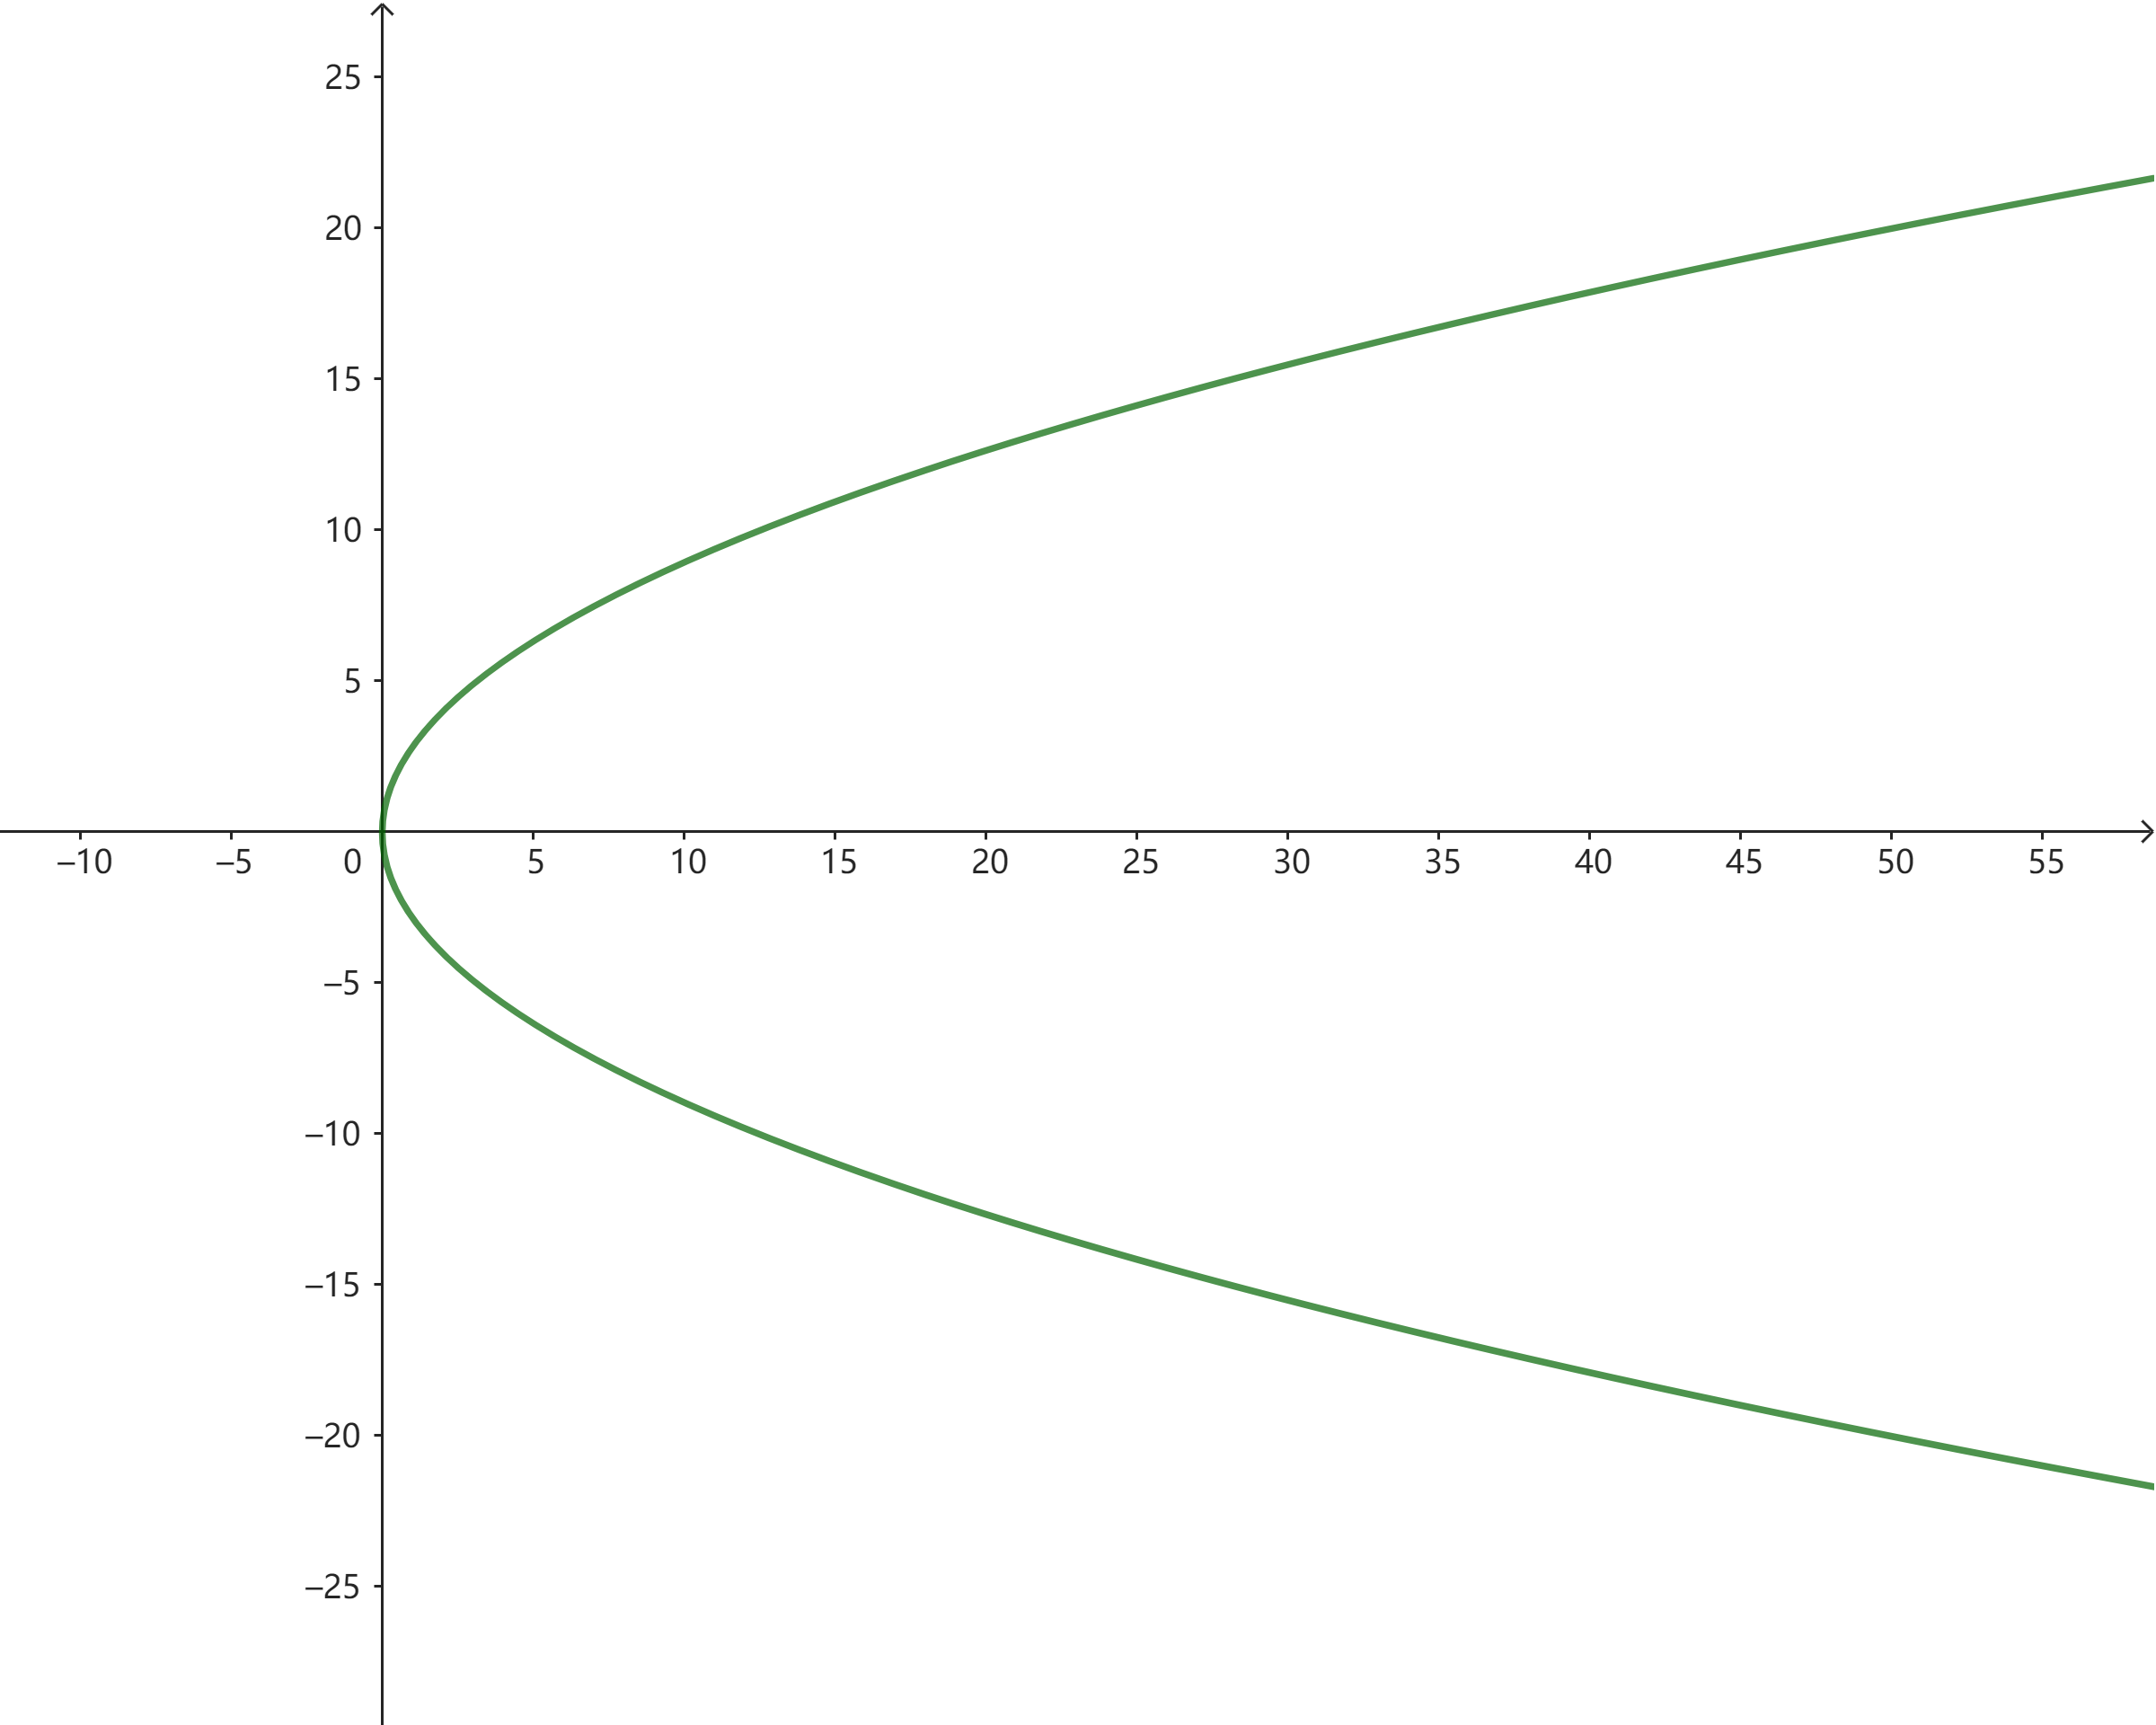
\includegraphics[width=0.3\textwidth]{tu/抛物线1.png}
\end{wrapfigure}

如果$AC = 0$,可以画出曲线如右图。这样的曲线称为抛物线。典型的抛物线方程可以写为:
$$ y^2 = 2px  \quad \mbox{(如右图)} $$
或
$$ x^2 = 2py  \quad \mbox{(如左下图)} \qquad  \qquad  \qquad  \qquad\;\;\; \phantom{123}$$
其中$p \neq 0$是描述抛物线的参数。

\begin{wrapfigure}[5]{l}{0.32\textwidth} %this figure will be at the right
    \vspace{-30pt}
    \flushright
    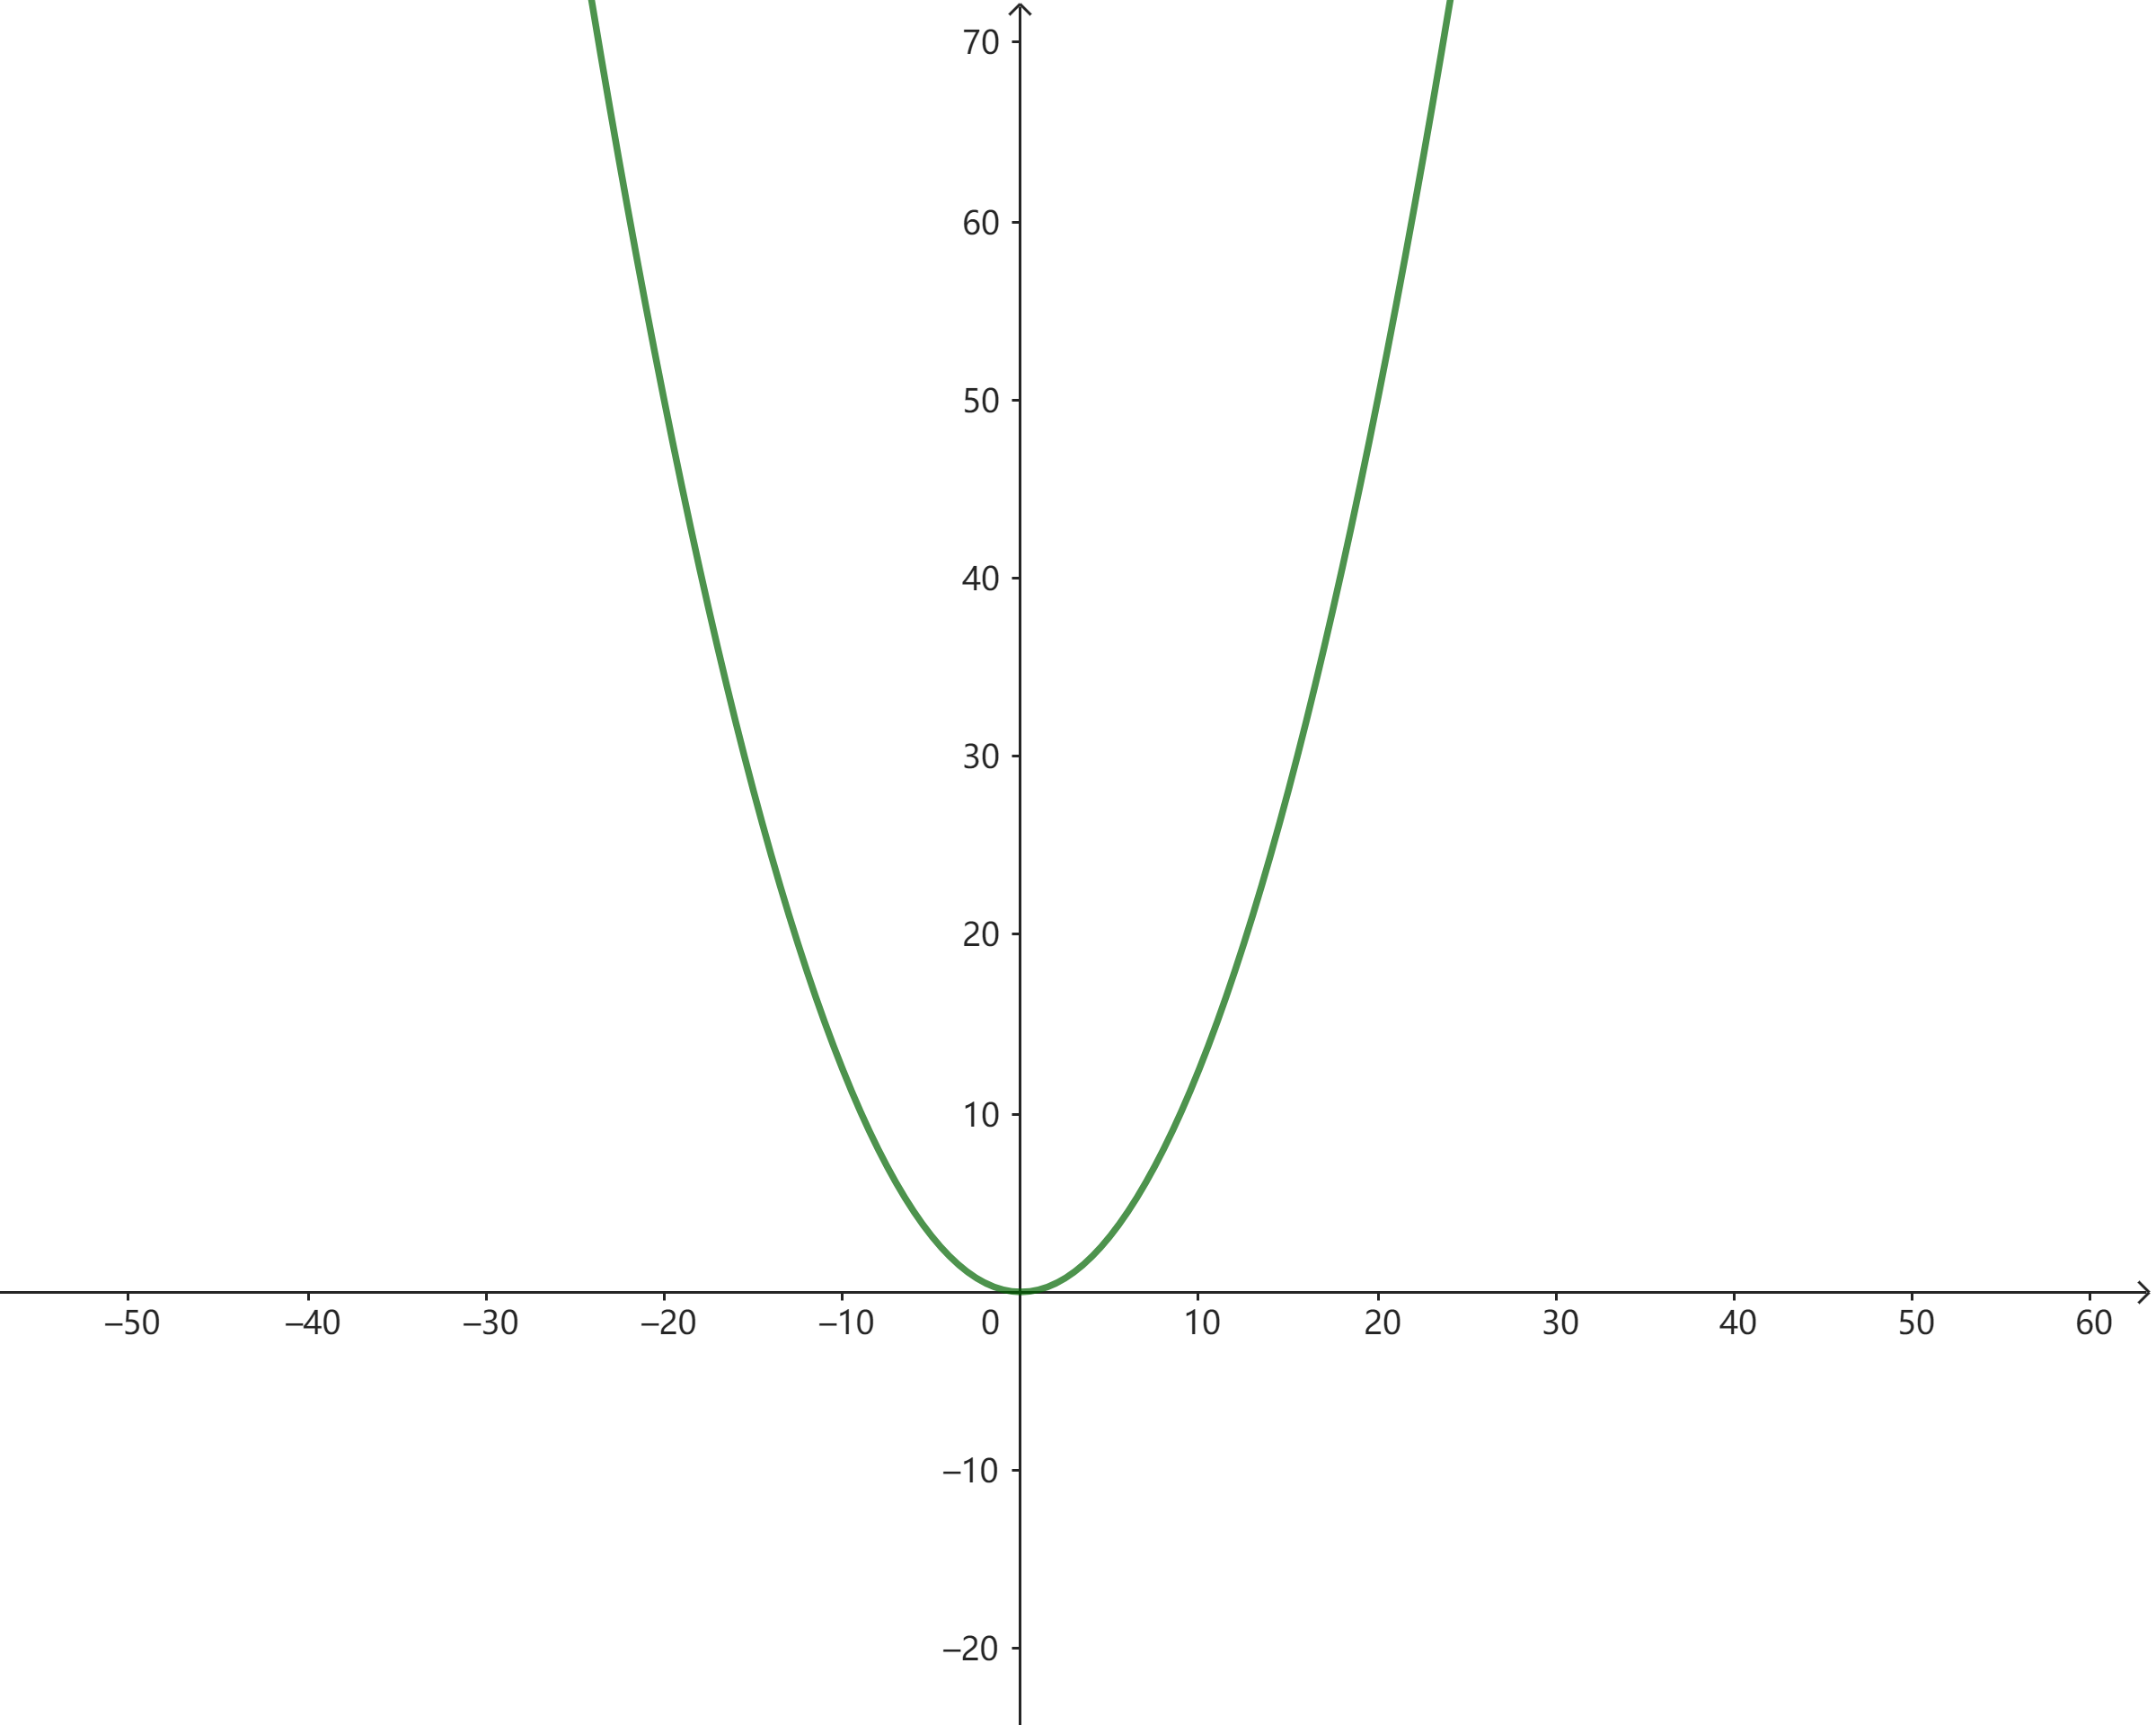
\includegraphics[width=0.3\textwidth]{tu/抛物线2.png}
\end{wrapfigure}

抛物线就是二次函数的曲线。按开口方向,抛物线可分为上下左右四类。它不是闭合曲线,也不是有界曲线,
恰有一条对称轴,与开口方向平行。

这三类曲线称为二次曲线。我们接下来会看到,一般的二次曲线要么是这三类曲线之一,要么是直线、点或空集(称为退化情形)。

考虑一般的二次曲线:
$$ Ax^2 + Bxy + Cy^2 + Dx + Ey + F = 0.$$

对于$B = 0$的情况,如果$AC\neq 0$,将曲线按向量$\displaystyle\left(-\frac{D}{2A},\,\,-\frac{E}{2C}\right)$平移,
就得到:
$$ Ax^2 + Cy^2 + F' = 0.$$
其中$F' = F - \frac{D^2}{4A} - \frac{E^2}{4C}$。两边除以$AC$并移项,得到:
$$ \frac{x^2}{C} + \frac{y^2}{A} = -\frac{F'}{AC}.$$
因此,根据$A$、$C$、$F'$的正负性,可以判断它或者是椭圆($A,C$同号,$A,F'$异号),
或者是双曲线($A,C$异号,$F' \neq 0$),或者是两条过原点直线($F' = 0$),或者是空集或单点集($A,C,F'$同号)。

如果$B = 0$,$A,C$中恰有一个为零,不妨设$A = 0$,则方程变为:
$$ Cy^2 + Dx + Ey + F = 0.$$

如果$D = 0$,则曲线方程变为关于$y$的二次方程,图像为$y = y_0$类型的水平线,条数等于方程实根的个数。

如果$D\neq 0$,按$\displaystyle\left(\frac{E^2 - 4CF}{4CD},\,\,-\frac{E}{2C}\right)$平移,就得到:
$$ Cy^2 = -Dx. $$
即
$$ y^2 = -\frac{D}{C}x. $$
因此曲线为抛物线。$C=0$而$A\neq 0$的情形也类同。

如果$B\neq 0$,我们希望通过某种变换,将方程转化为$B = 0$,即$xy$系数为$0$的情况。我们采用旋转变换。将坐标系逆时针旋转$\theta$角,
对应的旋转矩阵为:
$$
\begin{bmatrix}
    \cos{\theta} & -\sin{\theta} \\
    \sin{\theta} & \cos{\theta} 
\end{bmatrix}
$$
原坐标系中点$(x,\,\,y)$在新坐标系中坐标$(u,\,\,v)$满足:
$$
\begin{bmatrix}
    x \\ y
\end{bmatrix}
=
\begin{bmatrix}
    \cos{\theta} & -\sin{\theta} \\
    \sin{\theta} & \cos{\theta} 
\end{bmatrix}
\begin{bmatrix}
    u \\ v
\end{bmatrix}
= 
\begin{bmatrix}
    \cos{(\theta)}u - \sin{(\theta)}v \\ \sin{(\theta)}u + \cos{(\theta)}v
\end{bmatrix}
$$

% 双曲线、椭圆旋转后平移得到标准型

代入曲线方程,得到关于新坐标$(u,\,\,v)$的二次曲线方程,其中二次项为:
\begin{align*}
    Ax^2 + Bxy + Cy^2 &= A(\cos{(\theta)}u - \sin{(\theta)}v)^2 \\
    &\quad + B(\cos{(\theta)}u - \sin{(\theta)}v)(\sin{(\theta)}u + \cos{(\theta)}v) \\
    &\quad + C(\sin{(\theta)}u + \cos{(\theta)}v)^2 \\
    &= (A\cos^2{\theta} + B\cos{\theta}\sin{\theta} + C\sin^2{\theta})u^2 \\
    &\quad + (A\sin^2{\theta} - B\cos{\theta}\sin{\theta} + C\cos^2{\theta})v^2 \\
    &\quad + 2\cos{\theta}\sin{\theta}(C - A) + B(\cos^2{\theta} - \sin^2{\theta})uv
\end{align*}
$uv$的系数为:
$$ (C - A)\sin{(2\theta)} + B\cos{(2\theta)} $$
我们希望它等于$0$。

根据假设,$B\neq 0$。
如果$A = C$,那么取$\theta = \frac{\pi}{4}$即可。这时$u^2$、$v^2$的系数分别为
$$ A + \frac{B}{2}, \qquad A - \frac{B}{2}. $$
计算两者乘积,可以发现,两者同号(异号)当且仅当$4AC - B^2$大于(小于)零。

如果$A\neq C$,那么取
$$\theta = \theta_c = \frac{1}{2} \arctan{\frac{B}{A - C}},$$

% \begin{align*}
%     \cos{(2\theta_c)} &= \frac{A - C}{\Delta} \\
%     \sin{(2\theta_c)} &= \frac{B}{\Delta}  \\
%     \Delta &= \sqrt{B^2 + (A - C)^2}
% \end{align*}

% \begin{align*}
%     &\;A\cos^2{(\theta_c)} + B\cos{\theta}\sin{\theta} + C\sin^2{\theta} \\
%    =&\;\frac{A+C}{2} + \frac{A-C}{2}\cos{(2\theta_c)} + \frac{B}{2}\sin{(\theta_c)} \\
%    =&\;\frac{A+C}{2} + \frac{A-C}{2}\frac{A - C}{\Delta} + \frac{B}{2}\frac{B}{\Delta} \\
%    =&\;\frac{A+C}{2} + \frac{1}{2\Delta}\left((A - C)^2 + B^2\right) \\
%    =&\;\frac{A+C}{2} + \frac{\Delta^2}{2\Delta} \\
%    =&\;\frac{A+C}{2} + \frac{\Delta}{2} \\
% \end{align*}

则$uv$的系数为$0$。这时$u^2$、$v^2$的系数分别为:
$$ \frac{A+C}{2} + \frac{\sqrt{B^2 + (A - C)^2}}{2}, \qquad \frac{A+C}{2} - \frac{\sqrt{B^2 + (A - C)^2}}{2}. $$
计算两者乘积,可以发现,两者同号(异号)仍然当且仅当$4AC - B^2$大于(小于)零。

综上所述,任何二次曲线都可以通过旋转和平移,转变为典型的三类曲线之一,或退化情形。
也就是说,任何二次曲线,只要是“弯的”,就必然是椭圆、双曲线,或抛物线\footnote{我们约定圆是椭圆的特殊情形。}。
对于一般的二次曲线,我们可以用二次项的系数来直接判定它属于哪一类。
\begin{itemize}
    \item 如果$B^2<4AC$,那么二次曲线为\textbf{椭圆类型}(椭圆、圆或退化情形);
    \item 如果$B^2>4AC$,那么二次曲线为\textbf{双曲类型}(双曲线或退化情形);
    \item 如果$B^2=4AC$,那么二次曲线为\textbf{抛物线型}(抛物线或退化情形)。
\end{itemize}

\begin{sk}
    \mbox{} \\
    \indent 1. 列举所有二次曲线的退化情形,说明它们和椭圆、双曲线、抛物线的联系。\\
    \indent 2. 能否用矩阵和向量表示二次曲线的方程?这里的矩阵和直变换的矩阵有什么不同?
\end{sk}

\begin{xt}
    \mbox{} \\
    \indent 1. 将以下二次曲线转为标准形式:
    \begin{align*}
        1).& x^2 + xy +y^2 - 2x + 2y + 1 = 0,  &2).& 2x^2 + 3xy -y^2 - x = 0 \\
        3).& x^2 + 2xy + y^2 + 2x - 6y - 2 = 0,  & 4).& 2x^2 - \frac{7}{2}xy - y^2 - 3x - 3y - 2 = 0 
    \end{align*}
    \indent 2. 考虑一下附带变量系数$a$的二次曲线方程:
    $$ (1 - a)x^2 - \sqrt{1 - a^2}xy - ay^2 - x + (2a - 1)y + 1 - 2a = 0. $$
    根据$a$的不同取值,判断曲线的形状。
\end{xt}

\section{二次曲线的性质}

让我们来研究三类二次曲线:椭圆、双曲线、抛物线。历史上,数学家是通过直观的性质来发现并定义它们的。

首先,二次曲线可以通过到定点(定直线)的距离定义。

设配备直角坐标系$xOy$的平面上有两点$F_1:(-c,\,\,0)$和$F_2:(c,\,\,0)$。

考虑到这两点距离之和为$2a$的点的轨迹($a\geqslant c$)。

设平面上有点$P(x, \,\,y)$,它到$F_1$、$F_2$距离之和为$2a$,可列出方程:
$$ \sqrt{(x + c)^2 + y^2} + \sqrt{(x - c)^2 + y^2} = 2a.$$
移项平方:
\begin{align*}
    (x + c)^2 + y^2 &= (2a - \sqrt{(x - c)^2 + y^2})^2 = 4a^2 - 4a\sqrt{(x - c)^2 + y^2} + (x - c)^2 + y^2 \\
    4a\sqrt{(x - c)^2 + y^2} &= 4a^2 - 4cx.
\end{align*}
再平方,得到:
\begin{align*}
    (x - c)^2 + y^2 &= \left(a - \frac{cx}{a}\right)^2 \\
    (1 - \frac{c^2}{a^2})x^2 + y^2 &= a^2 - c^2.
\end{align*}
如果$a = c$,则得到$y = 0$,从而$-c \leqslant x \leqslant c$,轨迹为线段$F_1F_2$。

如果$a > c$,则得到:
$$ \frac{x^2}{a^2} + \frac{y^2}{a^2 - c^2} = 1.$$
记$b = \sqrt{a^2 - c^2}$,则得到$P$属于椭圆:
$$ \frac{x^2}{a^2} + \frac{y^2}{b^2} = 1.$$

反之,设$P$为椭圆上的点,则它到$F_1$、$F_2$的距离之和为:
\begin{align*}
    &\;\sqrt{(x + c)^2 + y^2} + \sqrt{(x - c)^2 + y^2}  \\
    =&\;\sqrt{(x + c)^2 + a^2 - c^2\left(1 - \frac{x^2}{a^2}\right)} + \sqrt{(x - c)^2 + a^2 - c^2\left(1 - \frac{x^2}{a^2}\right)} \\
    =&\;\sqrt{\frac{c^2x^2}{a^2} + 2cx + a^2} + v\sqrt{\frac{c^2x^2}{a^2} - 2cx + a^2} \\
    =&\; \left|a + \frac{cx}{a}\right| + \left|a - \frac{cx}{a}\right|
\end{align*}
由于$|x| \leqslant a$,所以$\displaystyle\left|\frac{cx}{a}\right| \leqslant c \leqslant a$,于是距离之和为
$2a$。

综上所述,$a>c$时,轨迹为椭圆。

也就是说,椭圆可以定义为平面上到两点距离之和为定值的点的轨迹。

\begin{figure}[h] 
    % \vspace{-4pt}
    \centering
    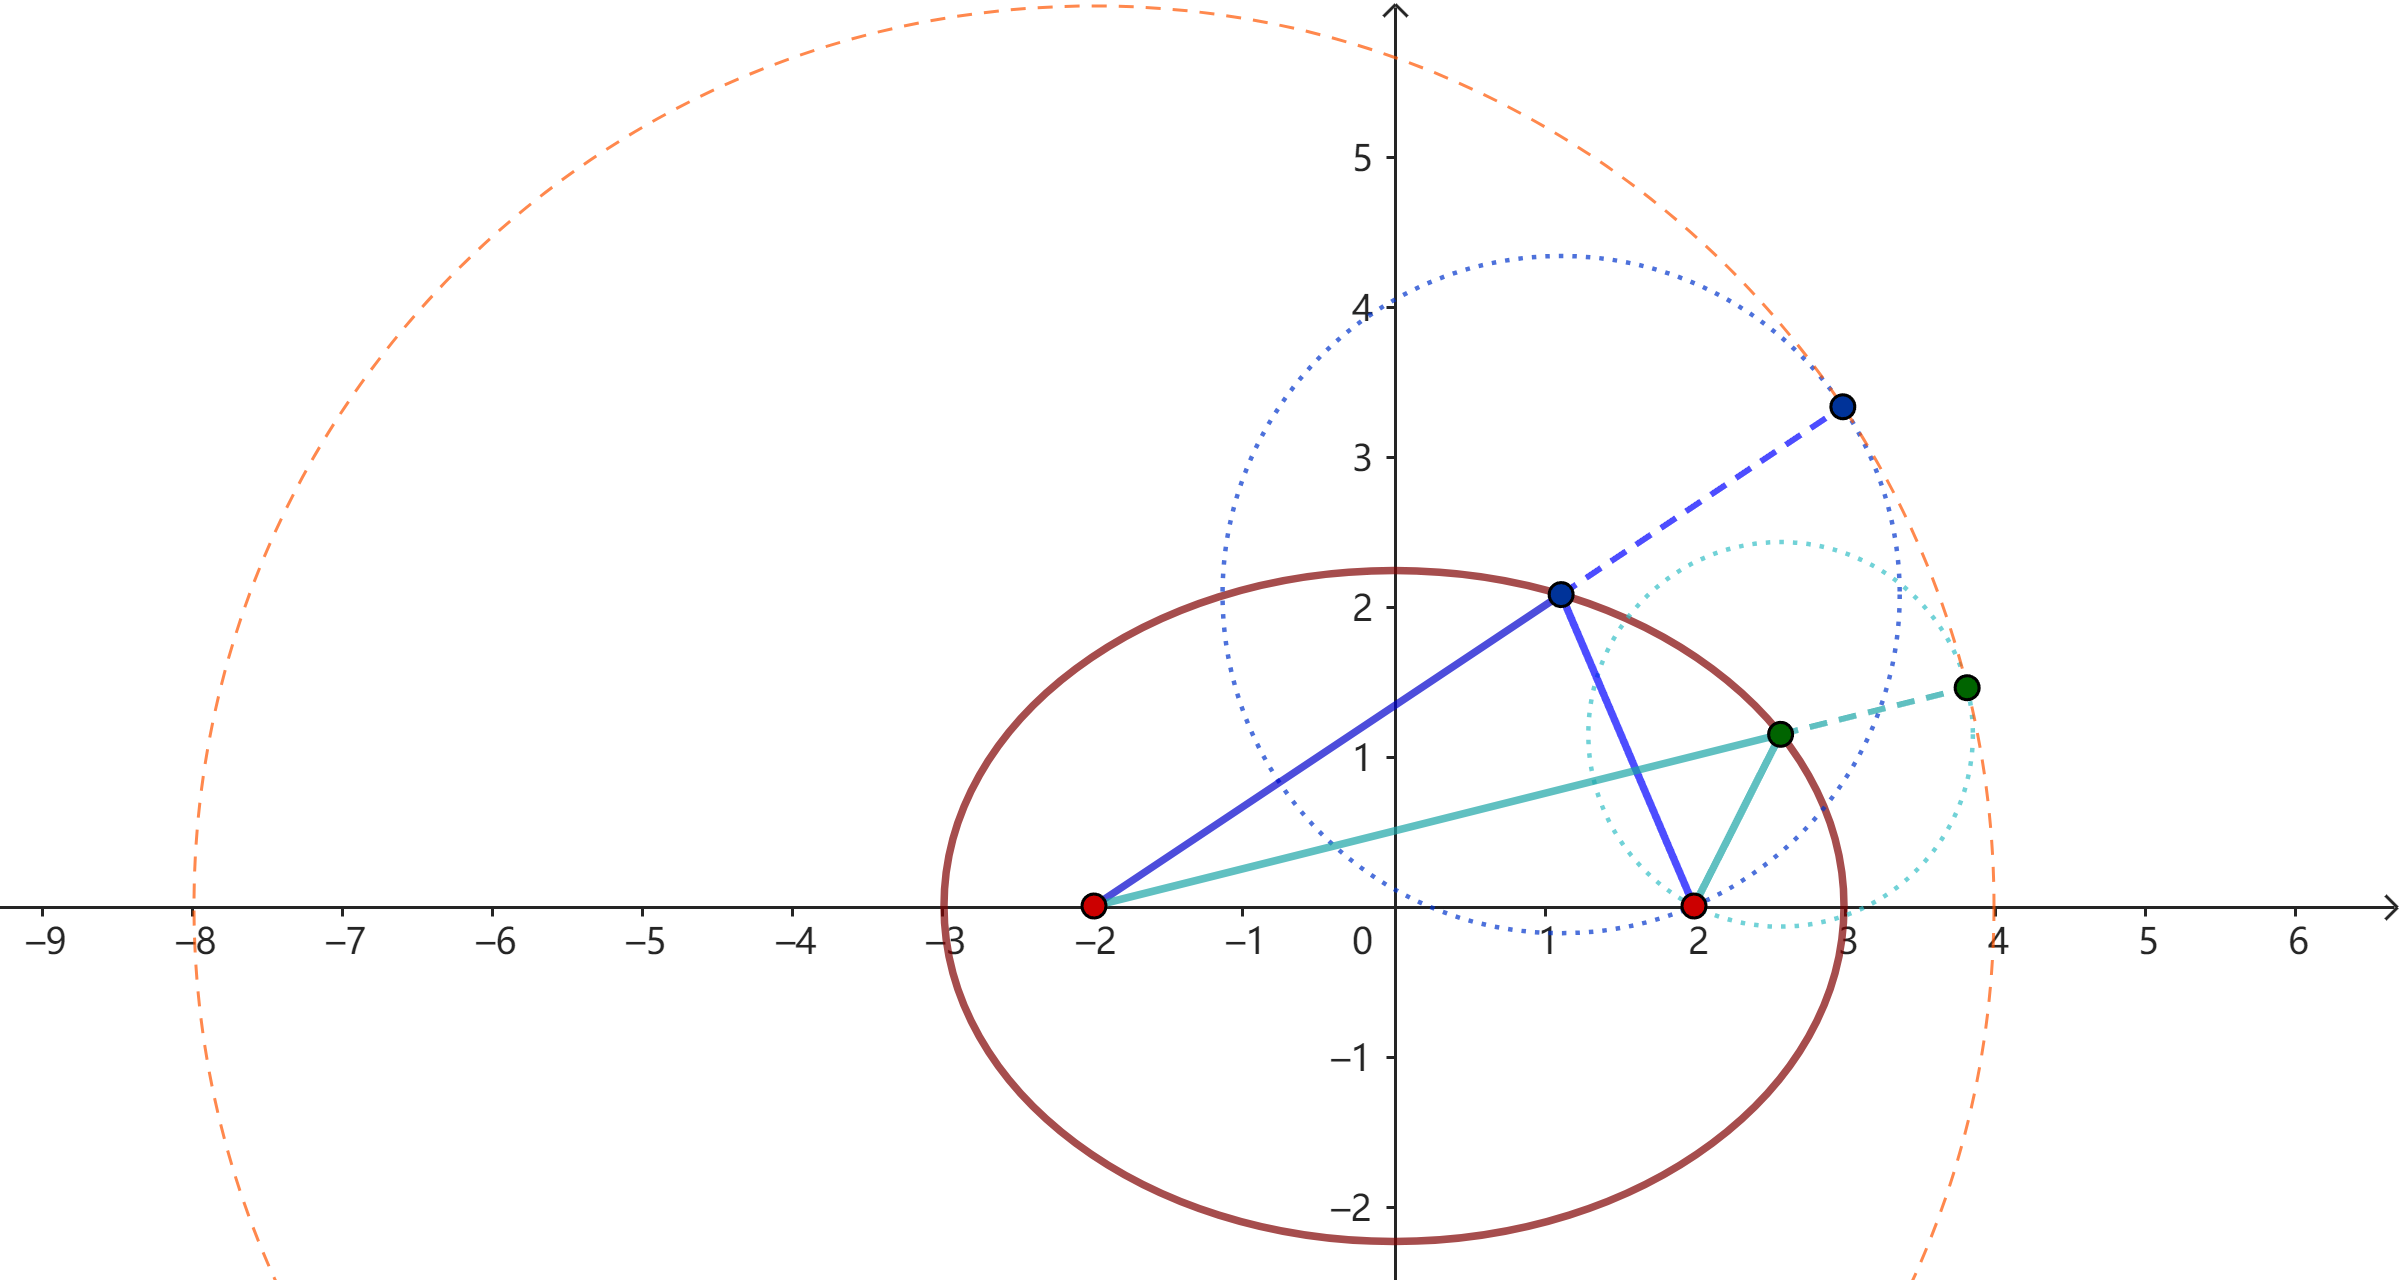
\includegraphics[width=0.8\textwidth]{tu/椭圆第一定义.png}
    \caption*{\texttt{到两点距离之和为定值的点的轨迹}}
\end{figure}

我们称$F_1$、$F_2$为椭圆的\textbf{焦点},$F_1F_2$中点为\textbf{椭圆中心},椭圆的\textbf{焦距}为$2c$。
椭圆与$x$轴、$y$轴的交点距离称为它的\textbf{长轴}和\textbf{短轴}。长轴、短轴分别为$2a$、$2b$(较大者为长轴)。

焦距和长轴之比$\displaystyle e =\frac{c}{a}$称为椭圆的\textbf{离心率}。离心率介于$0$和$1$之间。离心率越大,椭圆越狭长。离心率为$0$时,两焦点重合,椭圆就是圆。

再考虑到这两点距离之差为$2a$的点的轨迹($a\leqslant c$)。

设平面上有点$P(x, \,\,y)$,它到$F_1$、$F_2$距离之差为$2a$,可列出方程:
$$ \left|\sqrt{(x + c)^2 + y^2} - \sqrt{(x - c)^2 + y^2}\right| = 2a.$$
同上解得:
\begin{align*}
    \left(1 - \frac{c^2}{a^2}\right)x^2 + y^2 &= a^2 - c^2.
\end{align*}
如果$a = c$,则得到$y = 0$,从而$x \leqslant -c$或$x \geqslant c$,轨迹为$F_1$、$F_2$向$x$轴两方的射线。

如果$a < c$,则得到:
$$ \frac{x^2}{a^2} - \frac{y^2}{c^2 - a^2} = 1.$$
记$b = \sqrt{c^2 - a^2}$,则得到$P$属于双曲线:
$$ \frac{x^2}{a^2} - \frac{y^2}{b^2} = 1.$$

反之,设$P$为双曲线上的点,则它到$F_1$、$F_2$的距离之差为:
\begin{align*}
    &\;\left|\sqrt{(x + c)^2 + y^2} - \sqrt{(x - c)^2 + y^2}\right|  \\
    =&\; \Bigg|\left|a + \frac{cx}{a}\right| - \left|a - \frac{cx}{a}\right|\Bigg|
\end{align*}
由于$|x| \geqslant a$,$x \geqslant a$或$x \leqslant -a$。

$x \leqslant -a$时,$\frac{cx}{a} < x \leqslant -a$,所以$\left|a + \frac{cx}{a}\right| = -\frac{cx}{a} - a$,
$\left|a - \frac{cx}{a}\right| = a - \frac{cx}{a}$,于是距离之差为$2a$。

$x \geqslant a$时,$\frac{cx}{a} > x \geqslant a$,所以$\left|a - \frac{cx}{a}\right| = \frac{cx}{a} - a$,
$\left|a + \frac{cx}{a}\right| = a + \frac{cx}{a}$,于是距离之差为$2a$。

所以距离之差总是$2a$。综上,平面上到两点距离之差为定值的点的轨迹是双曲线。以上两种情况分别对应双曲线的左右两支。
双曲线同样定义焦点、焦距、交点、中心和离心率$\displaystyle e =\frac{c}{a}$。$2a$、$2b$分别称为\textbf{实轴}、\textbf{虚轴}。

双曲线的离心率$e$大于$1$。离心率越大,双曲线两支越靠近,各自的开口越宽。

\begin{figure}[h] 
    % \vspace{-4pt}
    \centering
    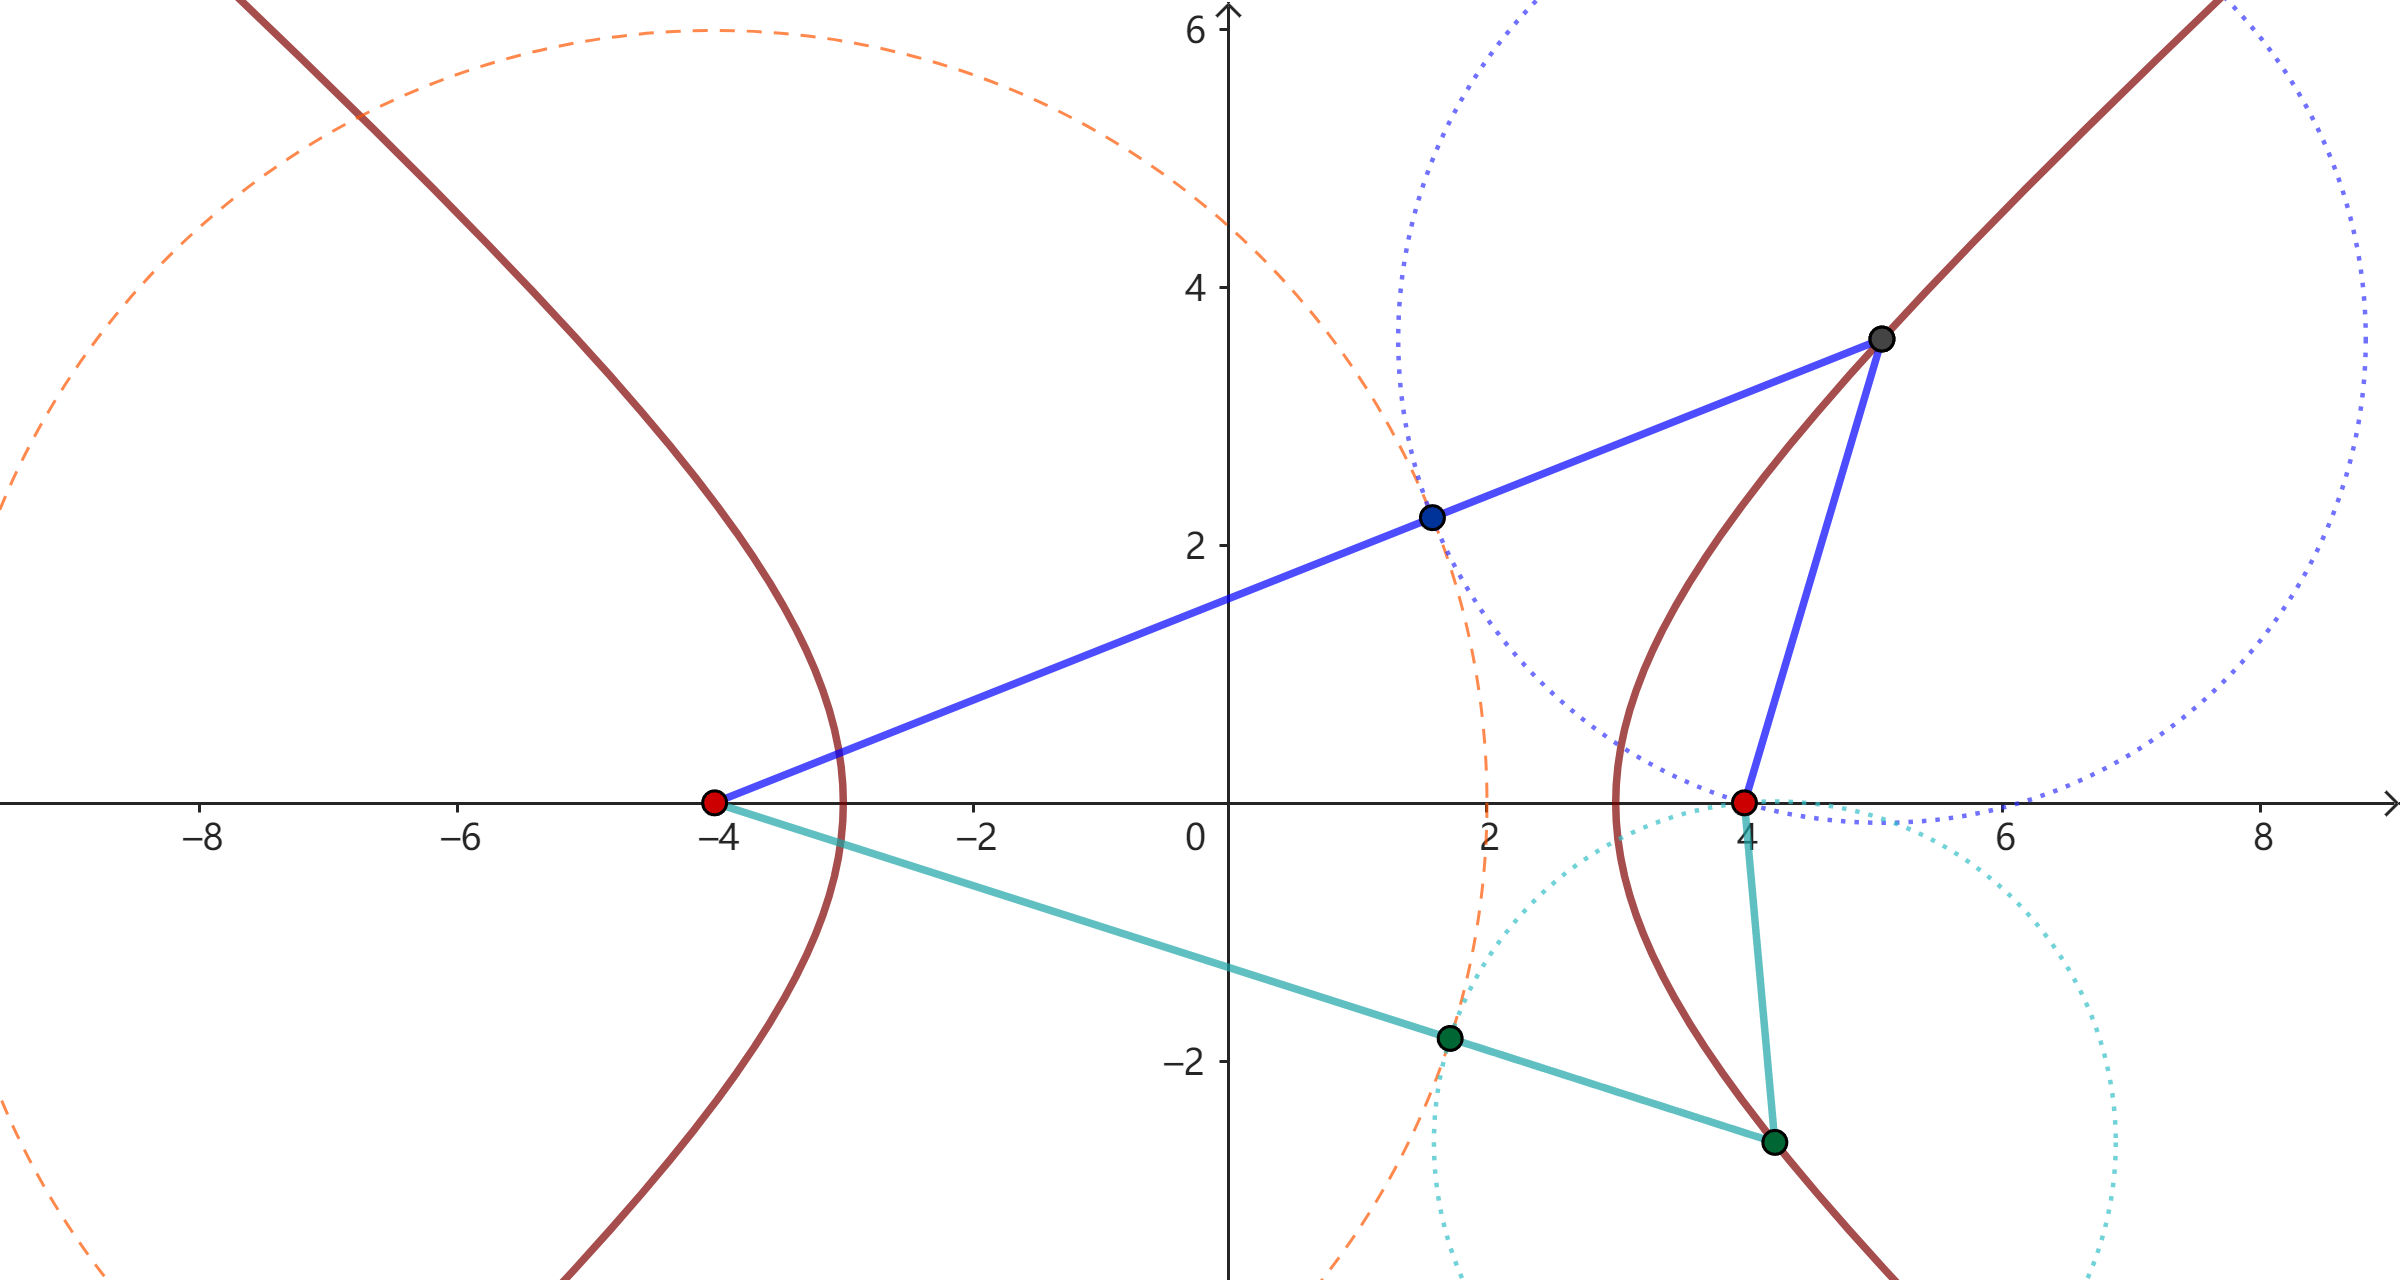
\includegraphics[width=0.8\textwidth]{tu/双曲线第一定义.png}
    \caption*{\texttt{到两点距离之差为定值的点的轨迹}}
\end{figure}

最后考虑到$F_2$和直线$x + c = 0$距离相等的点的轨迹。

设平面上有点$P(x, \,\,y)$,它到$F_2$和直线$x + c = 0$距离相等,可列出方程:
$$ \left|x + c\right| = \sqrt{(x - c)^2 + y^2}.$$
解得$P$属于抛物线:
$$ y^2 = 4cx.$$

反之,设$P$为抛物线上的点,则它到$F_2$的距离为:
\begin{align*}
    \sqrt{(x - c)^2 + y^2} &= \sqrt{(x - c)^2 + 4cx} = |x + c|.
\end{align*}
等于到直线$x + c = 0$的距离。

综上,轨迹为抛物线$ y^2 = 4cx$。抛物线是平面上到定点和定直线距离相等的点的轨迹。
$F_2$称为抛物线的\textbf{焦点}。$x + c = 0$称为抛物线的\textbf{准线}。

\begin{figure}[h] 
    % \vspace{-4pt}
    \centering
    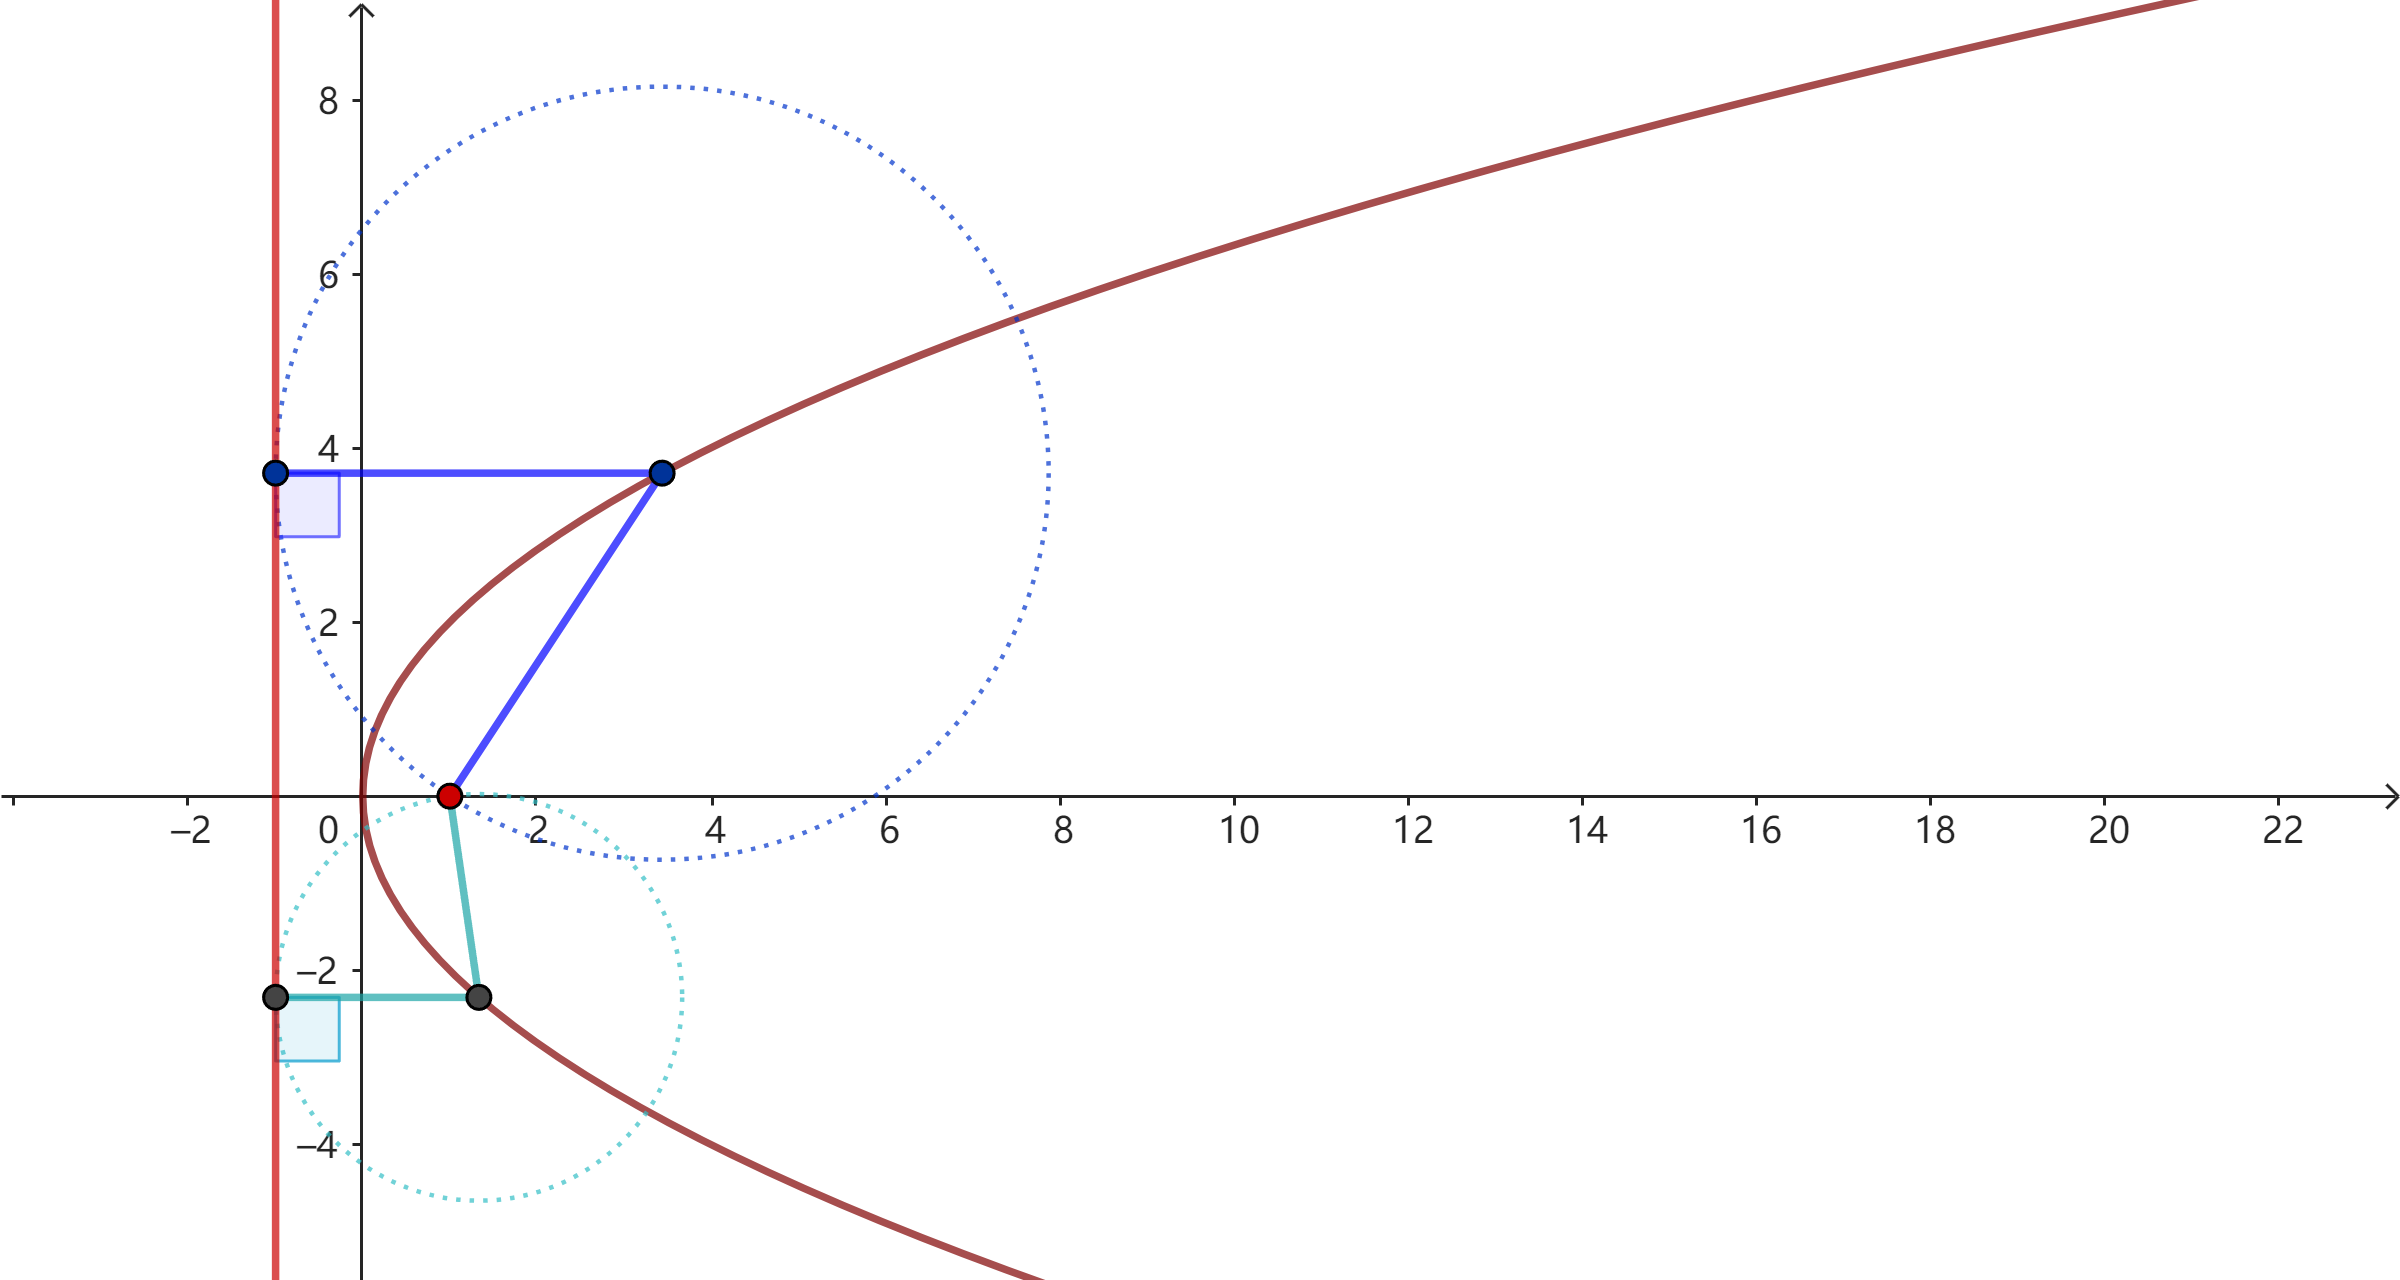
\includegraphics[width=0.8\textwidth]{tu/抛物线第一定义.png}
    \caption*{\texttt{到定点与定直线距离相等的点的轨迹}}
\end{figure}

以上是三类二次曲线的直观定义,也称为它们的\textbf{第一类定义}。

除此以外,我们还可以用另一种直观方式定义二次曲线。

考虑椭圆
$$ \frac{x^2}{a^2} + \frac{y^2}{b^2} = 1.$$
在前面的计算中,我们得到椭圆上一点$P(x,\,\,y)$到焦点$F_2$的距离之和为:
$$ \sqrt{(x - c)^2 + y^2} = \left|a - \frac{cx}{a}\right|.$$
其中$\frac{c}{a} = e < 1$是离心率。于是:
$$  \sqrt{(x - c)^2 + y^2} = e\left|x - \frac{a}{e}\right| . $$
也就是说,$|PF_2|$与$P$到直线$x = \frac{a}{e}$的距离的比值是定值$e$。
反之,如果某点$P:(x,\,\,y)$满足上面的方程,则可以解得:
$$ (x - c)^2 + y^2 = \frac{c^2x^2}{a^2} + a^2 -2cx.$$
于是
$$ \frac{x^2}{a^2} + \frac{y^2}{b^2} = 1.$$
这说明$P$的轨迹是椭圆。这说明椭圆可以定义为$|PF_2|$与$P$到直线$x = \frac{a}{e}$的距离的比值为定值$e<1$的点。

同样,我们也可以定义椭圆为$|PF_1|$与$P$到直线$x = -\frac{a}{e}$的距离的比值为定值$e<1$的点。

我们把以上两直线称为关于相应焦点的\textbf{准线}。椭圆可以定义为到定点和定直线距离之比为定值$e<1$的点。

对于双曲线,我们可以做类似的验证,双曲线也定义为到定点和定直线距离之比为定值的点,只不过定值$e > 1$。

综上,我们可以这样定义三类二次曲线。设有定点$F$、定直线$l$以及正数$e$。
考虑到$F$的距离和$l$的距离之比为$e$的点的轨迹,则:
\begin{itemize}
    \item $e<1$对应椭圆;
    \item $e = 1$对应抛物线;
    \item $e >1$对应双曲线。
\end{itemize}
我们把这种定义称为\textbf{二次曲线的第二类定义}。定义中的直线统一称为\textbf{准线}。

\begin{figure}[h] 
    % \vspace{-4pt}
    \centering
    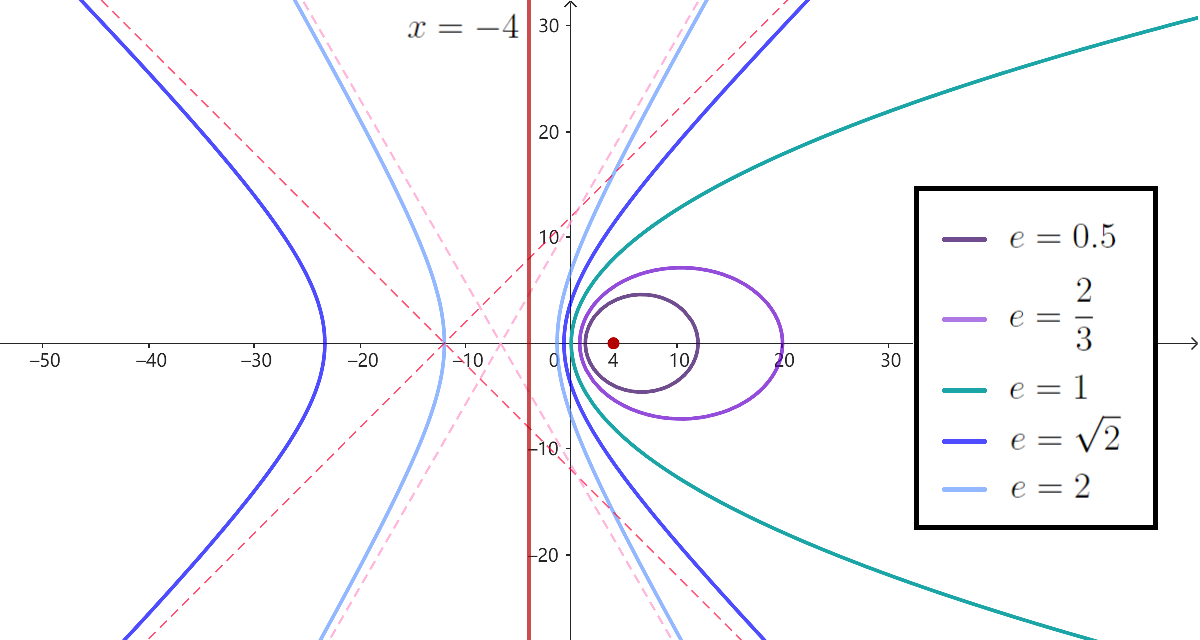
\includegraphics[width=0.8\textwidth]{tu/二次曲线第二定义1.png}
    \caption*{\texttt{到点}$(4,\,\,0)$\texttt{与到直线}$x=-4$\texttt{距离之比为}$e$\texttt{的点的轨迹}}
\end{figure}
以上的定义从平面上的点和直线出发。然而,二次曲线最古老的定义和一种空间形体——圆锥——有关,
因此二次曲线也称为\textbf{圆锥曲线}。从圆锥出发,如何得到二次曲线呢?

考虑配备了直角坐标系$Oxyz$的空间中过原点的直线:
$$ 
\left\{
    \begin{array}{cl}
        z &= kx \qquad (k > 0) \\
        y &= 0
    \end{array}
\right.
$$
以它为母线,绕$z$轴旋转,得到圆锥:
$$ k^2(x^2 + y^2) = z^2. $$

考虑平面$\gamma: \,\,z = ax + b$($a > 0$),设它截圆锥得到一个截面,我们考虑这个截面的边线。

为了研究截面的边线,我们绕$y$轴旋转坐标系,使新$x$轴平行于$\gamma$,新$z$轴方向向量为$\gamma$的法向量。
$xOz$平面上的基变更矩阵为:
$$
\begin{bmatrix}
    \frac{1}{\sqrt{a^2+1}} & -\frac{a}{\sqrt{a^2+1}} \\
    \frac{a}{\sqrt{a^2+1}} & \frac{1}{\sqrt{a^2+1}}
\end{bmatrix}
$$
于是$(x,\,\,y,\,\,z)$在新坐标轴里的坐标$(x',\,\,y',\,\,z')$满足:
$$
\begin{bmatrix}
    x \\ y \\ z
\end{bmatrix}
= 
\begin{bmatrix}
    \frac{x' - az'}{\sqrt{a^2+1}} \\ y' \\ \frac{ax' + z'}{\sqrt{a^2+1}}
\end{bmatrix}
$$
新坐标系中,平面$\gamma$的方程变为$z'=\frac{b}{\sqrt{a^2+1}}$,
而圆锥方程变为:
$$ k^2\frac{(x' - az')^2}{a^2+1} + k^2y^2 = \frac{(ax' + z')^2}{a^2+1} . $$
即:
$$ k^2(a^2+1)y'^2 + (k^2 - a^2)x'^2 - 2az'(1 + k^2)x' = (1 - a^2k^2)z'^2 $$
可以看到方程为二次曲线的方程。由于$y^2$的系数总大于零,$xy$项系数总为零,
$a<k$、$a=k$、$a>k$这三种情形分别对应三类二次曲线。

% 平面截圆锥得到二次曲线例图

直观来说,用平面截圆锥,就能得到二次曲线。二次曲线的类型取决于圆锥母线斜率和截面斜率的关系。
如果母线较陡($a<k$),则截面边线为椭圆;反之截面边线为双曲线。若两者斜率一样,则截面边线为抛物线。

\begin{sk}
    \mbox{} \\
    \indent 1. 用平面截圆锥、球体,会得到什么形状的截面?用圆锥面截圆锥、球体呢?\\
    \indent 2. 二次曲线的第一类、第二类定义让你想起实际中的哪些例子?它们和二次曲线是否相关?
\end{sk}

\begin{xt}
    \mbox{} \\
    \indent 1. 已知椭圆方程为
    $$ \frac{x^2}{9} + \frac{y^2}{4} = 1.$$
    \indent 1.1. 设椭圆两焦点为$F_1$、$F_2$。求$F_1$、$F_2$坐标。\\
    \indent 1.2. 过椭圆上一点$M$作椭圆的切线$PQ$。证明:$\angle F_1MP = \angle F_2MQ$。\\
    \indent 1.3. 以上结论是否对任意椭圆成立?\\
    \indent 2. 已知双曲线方程为
    $$ \frac{x^2}{9} - \frac{y^2}{7} = 1.$$
    \indent 2.1. 设双曲线两焦点为$F_1$、$F_2$。求$F_1$、$F_2$坐标。\\
    \indent 2.2. 过双曲线上一点$M$作双曲线的切线$PQ$。证明:$PQ$平分$\angle F_1MF_2$。\\
    \indent 2.3. 以上结论是否对任意双曲线成立?\\
    \indent 3. 已知抛物线方程为
    $$ y^2 = 8x.$$
    \indent 3.1. 求抛物线焦点$F$的坐标。\\
    \indent 3.2. 过抛物线上一点$M$作双曲线的切线$PQ$;过$M$作准线的垂线,交准线于$T$。证明:$PQ$平分$\angle FMT$。\\
    \indent 3.3. 以上结论是否对任意抛物线成立?\\
    \indent 4. 已知椭圆方程为
    $$ \frac{x^2}{4} + \frac{y^2}{3} = 1.$$
    一点到椭圆的\textbf{切线}定义为过该点且与椭圆只有一个交点的直线。\\
    \indent 4.1. 过点$P(4, 1)$作到椭圆的切线。证明这样的切线恰有两条。\\
    \indent 4.2. 给出两条切线的方程,以及两切点$Q_1$、$Q_2$坐标。\\
    \indent 4.3. 证明:直线$Q_1Q_2$经过椭圆的一焦点$F$,且$PF\perp Q_1Q_2$。\\
    \indent 4.4. 以上结论是否对任意点及任意椭圆成立?\\
    \indent 5.已知双曲线方程为
    $$ \frac{x^2}{4} - \frac{y^2}{5} = 1.$$ 
    一点到双曲线的\textbf{切线}定义为过该点且与双曲线只有一个交点的直线。\\
    \indent 5.1. 过点$P\left(1, \frac{4}{3}\right)$作到双曲线的切线。证明这样的切线恰有两条。\\
    \indent 5.2. 给出两条切线的方程,以及两切点$Q_1$、$Q_2$坐标。\\
    \indent 5.3. 证明:直线$Q_1Q_2$经过双曲线的一焦点$F$,且$PF\perp Q_1Q_2$。\\
    \indent 5.4. 以上结论是否对任意点及任意双曲线成立?\\
    \indent 6.已知抛物线方程为
    $$ y^2 = 4x.$$ 
    一点到抛物线的\textbf{切线}定义为过该点且与抛物线只有一个交点的直线。\\
    \indent 6.1. 过点$P(-1, -3)$作到抛物线的切线。证明这样的切线恰有两条。\\
    \indent 6.2. 给出两条切线的方程,以及两切点$Q_1$、$Q_2$坐标。\\
    \indent 6.3. 证明:直线$Q_1Q_2$经过抛物线的焦点$F$,且$PF\perp Q_1Q_2$。\\
    \indent 6.4. 以上结论是否对任意点及任意抛物线成立?\\
    
\end{xt}

\section{曲线与函数}

给定平面的曲线,比如椭圆的方程:
$$ \frac{x^2}{a^2} + \frac{y^2}{b^2} = 1,$$
如何研究它的性质呢?

如果曲线是函数的图像,我们可以通过研究微变率,分析它的增减、凹凸性质,可以将它在局部展开,近似为整式函数。
对于一般的曲线,我们也希望能将它转化为函数图像曲线。

曲线无法视为函数的图像,往往是因为多值,即同一个$x$值对应了多个$y$值。
我们可以只取曲线的一部分,将它视为函数的曲线。

具体来说,设曲线$\gamma$的方程为:
$$ F(x, \,\, y) = 0. $$
其中$F$是关于坐标$x$和$y$的多元函数。曲线$\gamma$就是满足方程$F$的点$(x,\,\,y)$的集合。

如果对于某些$x$的值,$F(x, \,\,y) = 0$有唯一解,就是说约束条件$F$将其对应到唯一的$y$。
这时,我们可以认为$y$是关于$x$的函数。这样的函数,称为由$F$确定的\textbf{隐函数}。

\begin{wrapfigure}[10]{r}{0.52\textwidth} %this figure will be at the right
    \vspace{-30pt}
    \flushright
    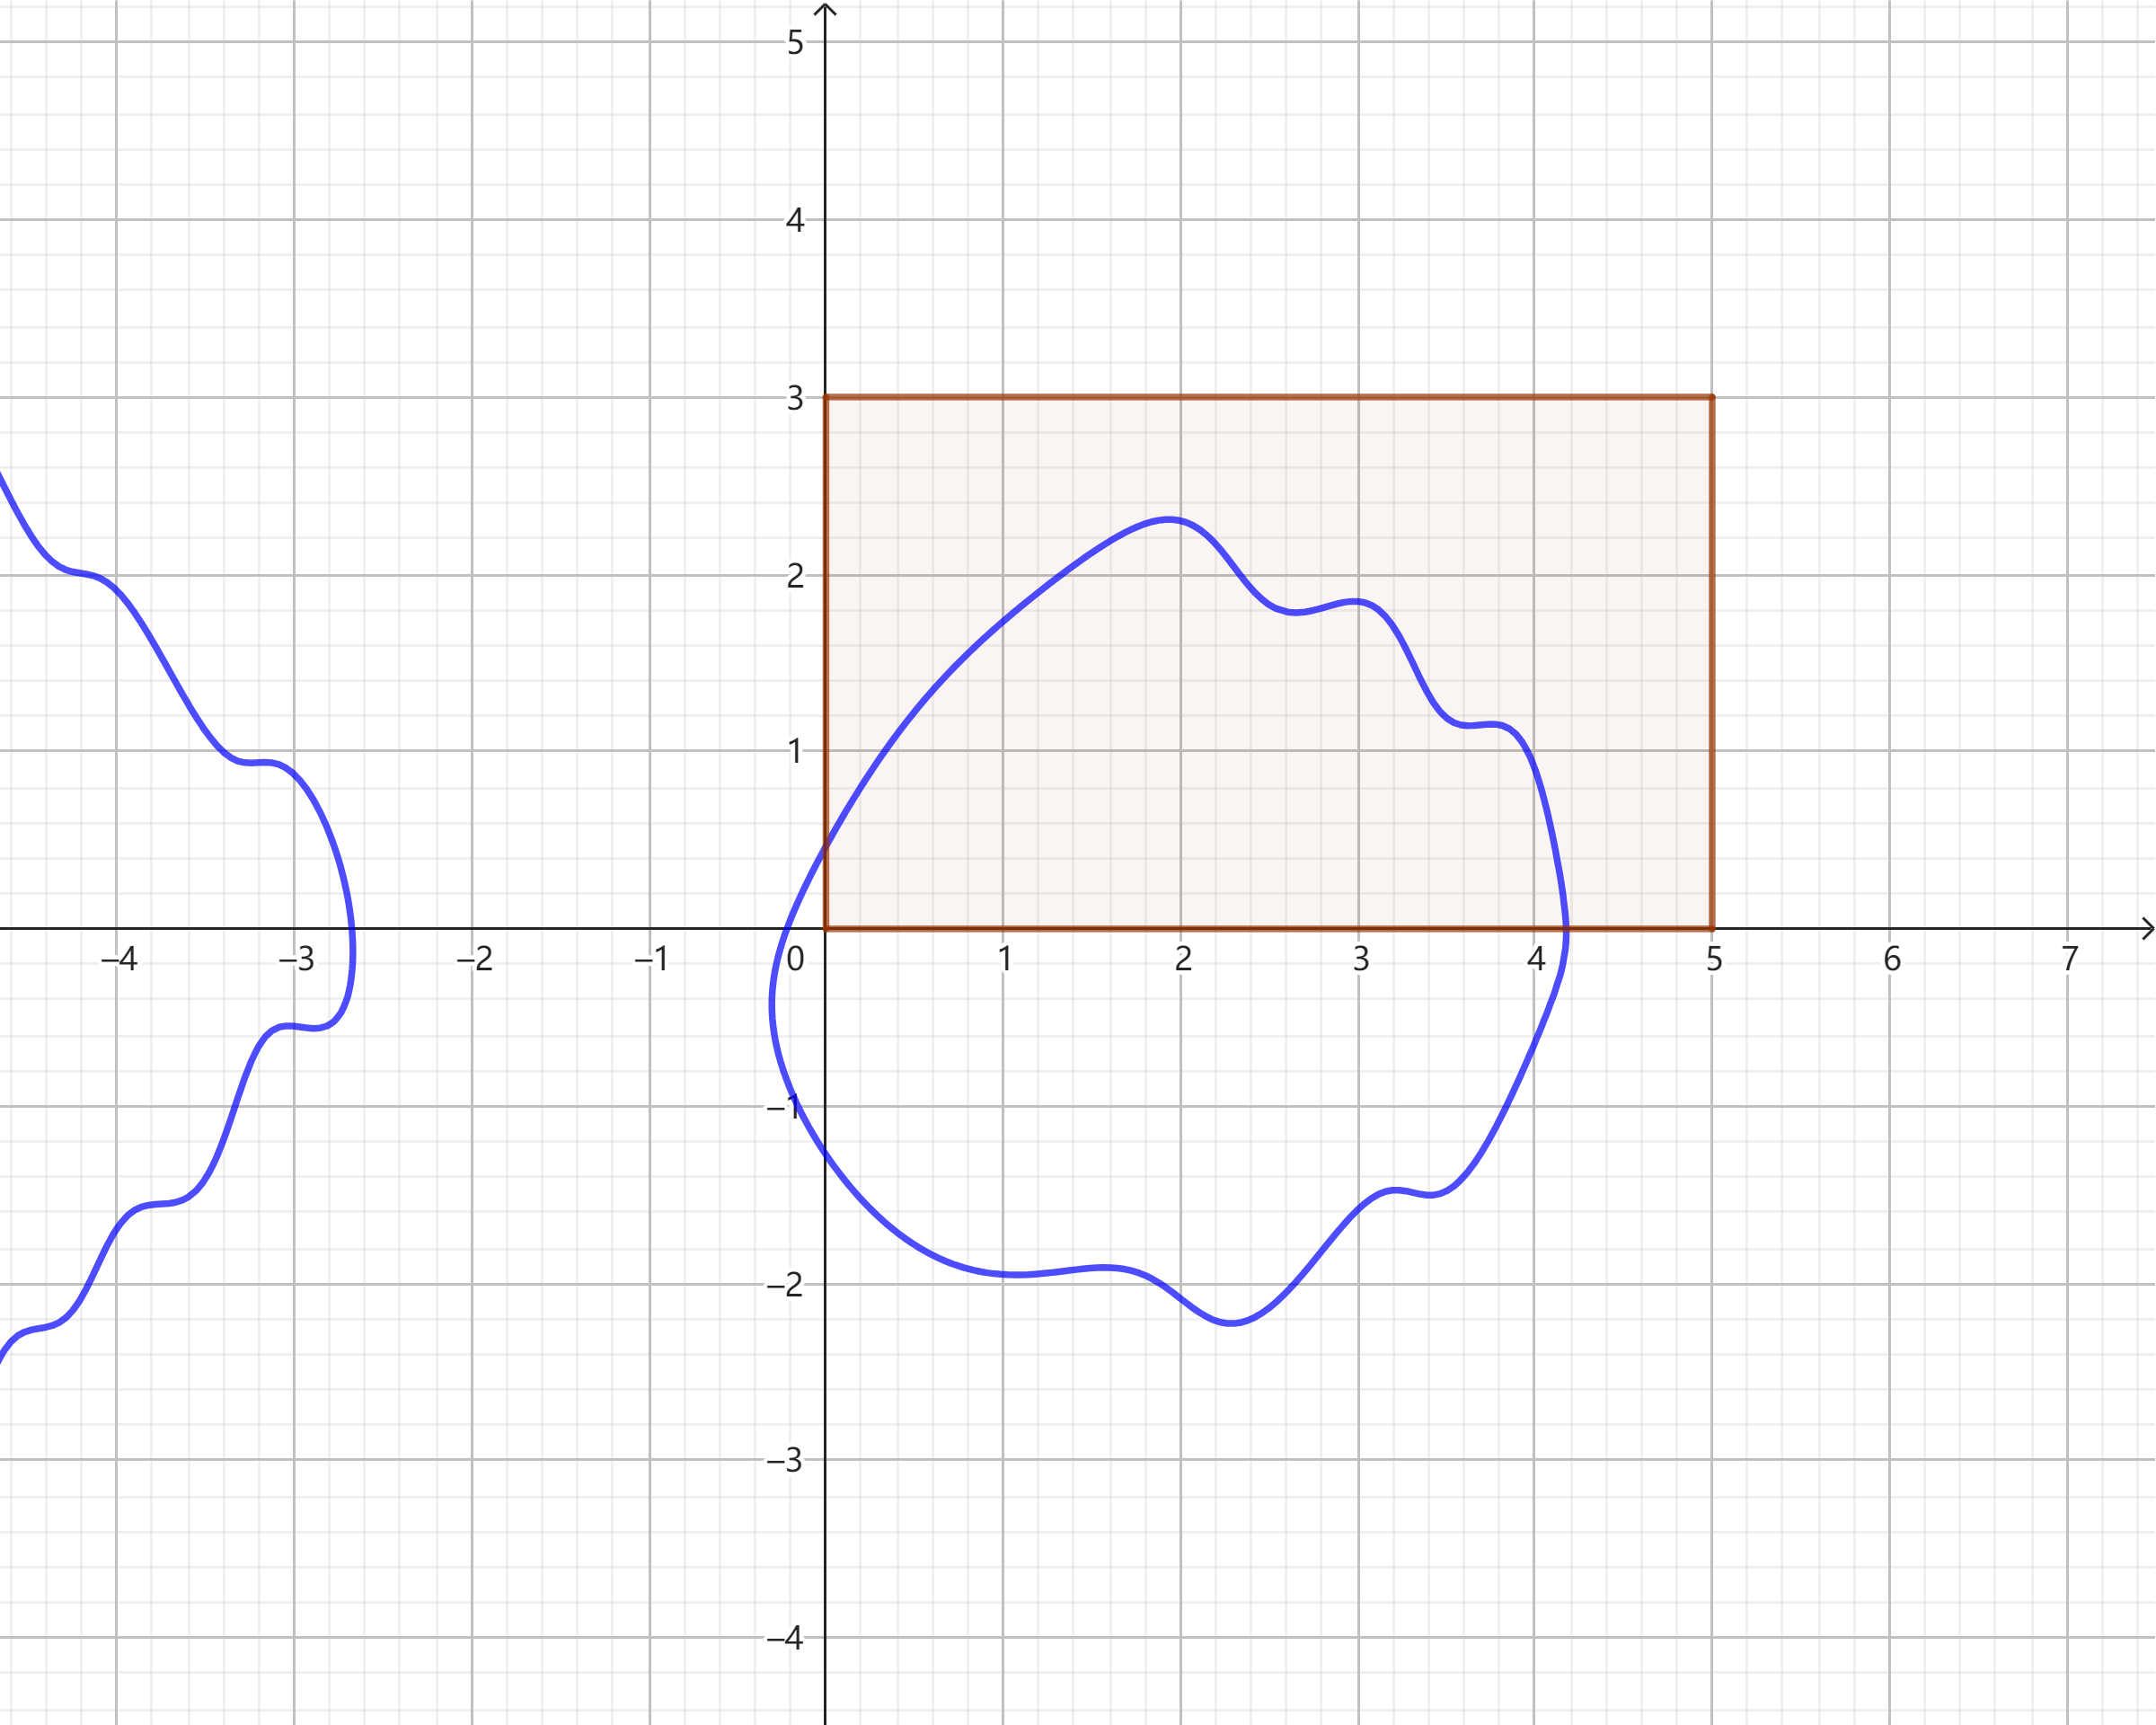
\includegraphics[width=0.5\textwidth]{tu/复杂平面曲线.png}
    \caption*{\texttt{取曲线的一部分,看作函数的曲线}}
\end{wrapfigure}

之所以称为隐函数,是因为我们并不能自动获得隐函数的表达式。
换句话说,我们并不一定知道怎样用$x$表示$y$。我们只知道,
对于$x$来说,$F(x, \,\,y) = 0$有唯一解。这个唯一解就是隐函数的值。

一般来说,使得$F(x, \,\,y) = 0$有唯一解的$x$不一定存在。于是,我们指定平面的子集,
使得$F(x, \,\,y) = 0$在子集中有唯一解。这样就可以确定$y$是关于$x$的隐函数。

以上面给出方程的椭圆为例子。我们知道,椭圆关于$x$轴对称,因此,对每个$x$,都有两个$y$值满足方程,它们互为相反数。
不过,如果只看上半平面,$x$和$y$之间可以有函数关系:
$$ \forall -a\leqslant x \leqslant a, \,\,\, y = b\sqrt{1 - \frac{x^2}{a^2}}= \frac{b}{a}\sqrt{a^2 - x^2}. $$
这就是由$F$确定的隐函数。

综上,对于无法整体视为函数图像的曲线,我们可以通过把平面拆分为子集的方法,把曲线的一部分视为函数图像。
这样的函数称为由曲线方程确定的\textbf{显化函数}。通过研究显化函数,我们可以讨论曲线的性质。

以椭圆为例。通过截取上半平面,我们得到了椭圆上半部分的显化函数:
$$ f: x\mapsto y = \frac{b}{a}\sqrt{a^2 - x^2}, \quad x \in [-a; a].  $$
对$f$求微变可得:
$$ \partial f(x) = -\frac{bx}{a}(a^2 - x^2)^{-\frac{1}{2}}$$
微变函数在区间$(-a;0)$上严格单调递增,在$(0;a)$上严格单调递减。显化函数$f$在$0$处取得最大值。
曲线在$(x_0,\,\, y_0)$处的切线为:
\begin{align*}
    y &= f(x_0) + \partial f(x_0)(x - x_0) \\
    &= y_0 -\frac{bx_0}{a\sqrt{a^2 - x_0^2}}(x - x_0) \\
    &= y_0 - \frac{b^2x_0(x - x_0)}{a^2y_0} \\
    &= \frac{a^2y_0^2 + b^2x_0^2 - b^2x_0x}{a^2y_0} \\
\end{align*}
由于
$$ \frac{x_0^2}{a^2} + \frac{y_0^2}{b^2} = 1,$$
上式变为
$$ a^2y_0y +  b^2x_0x = a^2b^2. $$
即:
$$ \frac{x_0x}{a^2} + \frac{y_0y}{b^2} = 1.$$
这就是椭圆的切线方程。

对$f$求二次微变可得:
$$ \partial^2 f(x) = -\frac{ab}{(a^2 - x^2)^{\frac{3}{2}} }.$$
$\partial^2 f$在区间$(-a;a)$上总小于零,这说明曲线总是上凸的。

\begin{sk}
    \mbox{} \\
    \indent 1. 计算双曲线$\frac{x^2}{a^2} - \frac{y^2}{b^2} = 1$在某点$(x_0,\,\,y_0)$附近的显化函数和在该点的切线方程。如何选取平面的子集?\\
    \indent 2. 一般来说,如何判断$F(x,\,\, y) = 0$确定的曲线在某点$(x_0,\,\,y_0)$附近能通过选取合适的子集来找到显化函数?
\end{sk}

\section{复值函数}

学习复数的时候,我们把复数视为复平面上的点。对于平面上的曲线,我们也可以将它视作复平面上点的轨迹,
用自变量为实数、值为复数的映射表达它。我们把这样的函数称为\textbf{实变复值函数}。

举例来说:
\begin{align*}
    \mathbb{R} \;&\rightarrow \mathbb{C} \\
    t \;&\mapsto \cos{t} + \imath \sin{t}
\end{align*}
就是一个实变复值函数。它把实数$t$映射到复数$\cos{t} + \imath \sin{t}$。在复平面上看,随着$t$变化,
它的轨迹是单位圆。

一般来说,给定两个实函数$u,v$,就可以组成一个复值函数:
$$ t\mapsto u(t) + \imath v(t).$$
这与描述平面曲线的参变映射是一样的。

除此以外,常见的经典函数是否能成为复值函数呢?比如,以下的写法是否可行呢?
\begin{align*}
    t &\mapsto \e^{\imath t} \\
    t &\mapsto \imath^t \\
    t &\mapsto \sin{\imath t} \\
    t &\mapsto \ln{\imath t} 
\end{align*}
这需要我们补充经典函数关于复数的定义,比如$\imath$的乘方、$\imath$次方、$\imath$的正弦、$\imath$的对数是什么意思。

要注意的是:以上这些定义都不是天然存在的。现实中并没有像整数的乘方那样,让我们抽象出$\imath$的乘方、$\imath$次方的实例。
但如果我们回忆实数特别是无理数次数的乘方,会发现,它也是我们“自作主张”定义的。
自然界里并没有“$\sqrt{2}$次方”。我们为了把幂函数作为实函数进行讨论,希望给每个实数自变量都赋予一个函数值,所以定义了“无理数次方”。
而我们对作为实函数的幂函数的要求是连续。事实上,我们定义的幂函数不仅连续,而且可微、光滑,具有很好的性质。

那么,我们是否也可以定义出满足某些良好性质的复值整式函数、复值幂函数呢?这种研究称为\textbf{实函数的复化}。
具体来说,我们希望找出某两个实函数$u,v$,使得由上定义的复值函数:
$$ t\mapsto u(t) + \imath v(t)$$
满足我们对$t\mapsto \e^{\imath t}$函数性质的某些期望。

比如,参考函数$t\mapsto \e^{at}$的性质,我们希望$f: t\mapsto \e^{\imath t}$满足:
\begin{enumerate}
    \item $f(0) = 1$;
    \item $\forall x, y \; \in \mathbb{R}, f(x + y) = f(x)\cdot f(y)$;
    \item $f$是连续函数乃至光滑函数;
    \item $\partial f(x) = \imath f(x).$
\end{enumerate}
等等。

又比如,因为$\sin^2{t} + \cos^2{t} = 1$,我们希望有:
$$ \sin^2{(\imath t)} + \cos^2{(\imath t)} = 1 $$

回到$t\mapsto \e^{\imath t}$,是否有这样的复值函数呢?来看上面提到的复值函数:
\begin{align*}
    h: \;t \;\mapsto \cos{t} + \imath \sin{t}
\end{align*}
不难验证:$h(0) = 1$,且
$$ \forall \, x, y\; \in \mathbb{R}, \quad h(x + y) = h(x)\cdot h(y).$$

由于$\imath$是与自变量无关的常数,而正弦函数与余弦函数都是光滑函数,作为两者的直组合,$h$也是光滑函数。

最后,可以验证:
$$ \partial h(x) = \partial \cos{(x)} + \imath \partial \sin{(x)} = - \sin{x} + \imath \cos{x} = \imath h(x) $$

这样看来,$h$似乎就是一个很好的候选。如果我们定义:
$$ \forall \, t \; \in \mathbb{R}, \quad  \e^{\imath t} = \cos{t} + \imath \sin{t}, $$
那么它满足前面我们希望它满足的所有性质。

用归纳法可以验证,对任何自然数乃至整数$n$,有
$$ \e^{n\imath t} = \cos{nt} + \imath \sin{nt} = (\cos{t} + \imath \sin{t})^n = \left( \e^{\imath t} \right)^n. $$
进一步有:
$$ \e^{\frac{\imath t}{n}} = \cos{\left(\frac{t}{n}\right)} + \imath \sin{\left(\frac{t}{n}\right)} = (\cos{t} + \imath \sin{t})^{\frac{1}{n}} = \left( \e^{\imath t} \right)^{\frac{1}{n}}. $$
从而对任何有理数$q = \frac{m}{n}$,都有:
$$ \e^{q\imath t} = \cos{qt} + \imath \sin{qt} = (\cos{t} + \imath \sin{t})^q = \left( \e^{\imath t} \right)^q. $$

一般来说,对实数$r$,可以定义:
$$ \forall \, t \; \in \mathbb{R}, \quad \e^{r\imath t} = \cos{rt} + \imath \sin{rt} = (\cos{t} + \imath \sin{t})^r = \left( \e^{\imath t} \right)^r. $$

可以看到,这样定义的复值指数函数的行为和实值指数函数有很大的不同。直观上来说,$t\mapsto \e^{t}$是单调递增的,而$t\mapsto \e^{\imath t}$是一个周期函数,它的轨迹在复平面上是单位圆。随着$t$的变化,函数绕着单位圆不断“转圈”。这是两种完全不同的行为。

比如,我们可以从上面推出:
$$ \e^{\frac{\imath\pi}{2}} = \imath, \quad \e^{\imath\pi} = -1, \quad \e^{\frac{3\imath\pi}{2}} = -\imath, \quad \e^{2\imath\pi} = 1. $$
换句话说,它的最小周期是$2\pi$。$\e^{\imath t}$和$\e^{\imath(2\pi + t)}$总是相等的。

再来看复值的对数函数。$\e^{\frac{\imath\pi}{2}} = \imath$启发我们,可以定义$\ln{\imath} = \frac{\imath\pi}{2}$。
这样定义似乎没什么问题,但我们发现:
$$ \e^{\frac{5\imath\pi}{2}} = \e^{\frac{\imath\pi}{2}} \times \e^{2\imath\pi} = \imath \times 1 = \imath. $$
于是又可以定义$\ln{\imath} = \frac{5\imath\pi}{2}$。一般来说,考虑复数$z$的“极坐标”表示:
$$ z = |z| \e^{\imath \theta}$$
其中$\theta$是$z$的幅角,那么可以定义
$$\ln{z} = \ln{|z|} + \theta \imath.$$
但复数的幅角$\theta$并不是唯一的。比如对任何整数$k$,$\theta + 2k\pi$也是$z$的幅角。因此,我们可以定义
$$\ln{z} = \ln{|z|} + \theta \imath + 2k\pi\imath.$$
然而,如果我们希望对数函数对复数也保持一些基本性质,比如:
$$ \ln{(z_1 \cdot z_2)} = \ln{z_1} + \ln{z_2}. $$
那么就需要有
$$ \ln{|z_1z_2|} + \theta \imath + 2k\pi\imath = \ln{|z_1|} + \theta_1 \imath + 2k_1\pi\imath + \ln{|z_2|} + \theta_2 \imath + 2k_2\pi\imath.$$
其中$\theta$是$z_1z_2$的幅角,$\theta_1, \theta_2$分别是$z_1, z_2$幅角,$k, k_1, k_2$是整数。

复数乘积的模等于模的乘积,因此问题在于幅角。以上关于幅角的关系总能成立吗?答案是否定的。
事实上,我们无法在复数域上完全保持$\ln{(z_1 \cdot z_2)} = \ln{z_1} + \ln{z_2}$的性质。
也就是说,复对数函数只能做到:
$$ \ln{(z_1 \cdot z_2)} \tong{2\pi} \ln{z_1} + \ln{z_2} . $$
这也是指数函数复化后性质改变的必然后果。复值指数函数不再是单调函数,而是周期函数。这使得作为反函数的对数函数无法保持所有的性质。

要注意的是,以上定义的复值指数函数,并不是从实变量的指数函数得来的,而是一个满足我们想象的条件的“候选”。这样定义是否有道理呢?是否与实变指数函数兼容呢?我们将在下一册继续研究。

\begin{et}
    设$t$为实数,给出与复值指数函数兼容的函数:$t\mapsto \sin{\imath t}$、$t\mapsto \cos{\imath t}$。
\end{et}

\begin{so}
    根据复值指数函数的定义,
    $$ \e^{\imath t} = \cos{t} + \imath \sin{t}, \qquad \e^{-\imath t} = \cos{t} - \imath \sin{t}. $$
    因此有:
    $$ \sin{t} = \frac{\e^{\imath t} - \e^{-\imath t}}{2\imath}.$$
    可以设想令
    $$ f(t) = \sin{\imath t} = \frac{\e^{\imath (\imath t)} - \e^{-\imath (\imath t)}}{2\imath} = \imath \frac{\e^{t} - \e^{-t}}{2}.$$
    同理,由于
    $$ \cos{t} = \frac{\e^{\imath t} + \e^{-\imath t}}{2},$$
    可以设想令
    $$ g(t) = \cos{\imath t} = \frac{\e^{\imath (\imath t)} + \e^{-\imath (\imath t)}}{2} = \frac{\e^{t} + \e^{-t}}{2}.$$
    可以验证:
    $$ f(0) = \sin{(\imath \cdot 0)} = 0, \quad g(0)=\cos{(\imath \cdot 0)} = 1,$$
    函数$f$、$g$都是光滑函数,且:
    \begin{align*}
        \partial f(t) &= \imath \frac{\e^{t} + \e^{-t}}{2} = \imath g(t) = (\partial\sin)(\imath t)\cdot (\partial(\imath t)), \\
        \partial g(t) &= \frac{\e^{t} - \e^{-t}}{2} = -\imath f(t) = (\partial\cos)(\imath t)\cdot (\partial(\imath t)).
    \end{align*}
    最后,它们满足:
    \begin{align*}
        \forall \; t\in \mathbb{R}, \quad & \sin^2{(\imath t)} + \cos^2{(\imath t)} = \left(\imath \frac{\e^{t} - \e^{-t}}{2}\right)^2 + \left( \frac{\e^{t} + \e^{-t}}{2}\right)^2 \\
        =\;& -\frac{\e^{2t} + \e^{-2t} - 2}{4} + \frac{\e^{2t} + \e^{-2t} + 2}{4} \\
        =\;& 1.
    \end{align*}
    但另一方面,$t\mapsto \sin{\imath t}$、$t\mapsto \cos{\imath t}$都不再是周期函数。

\end{so}

\begin{et}
    设$t$为实数,给出与复值指数函数兼容的幂函数:$t\mapsto t^{\imath}$。
\end{et}

\begin{so}
    关键是定义$z$为复数时,$a^{z}$是什么。对于实值指数函数,有:
    $$ a^{x} = \e^{x\ln{a}}. $$
    这启发我们把$a^{z}$表达为$\e^{z\ln{a}}$。于是我们可以试着定义:
    $$ t^{\imath} = \e^{\imath \ln{t}}. $$
    这个定义对正实数$t$有意义。它可以写为:
    $$ t^{\imath} = \cos{(\ln{t})} + \imath \sin{(\ln{t})} $$
    检查它是否满足幂运算法则。首先,对任意正实数$a,b$,计算$a^{\imath} \cdot b^{\imath}$:
    \begin{align*}
        a^{\imath} \cdot b^{\imath} &= (\cos{(\ln{a})} + \imath \sin{(\ln{a})}) \cdot (\cos{(\ln{b})} + \imath \sin{(\ln{b})}) \\
        &= \cos{(\ln{a} + \ln{b})} + \imath \sin{(\ln{a} + \ln{b})} \\
        &= \cos{(\ln{ab})} + \imath \sin{(\ln{ab})} \\
        &= (ab)^{\imath}
    \end{align*}
    另外,对任意实数$a$,定义:
    $$ t^{\imath a} = \e^{\imath a\ln{t}} $$
    这个定义与实值指数函数定义相容,且按这个定义,
    $$  t^{\imath a} = \cos{(a\ln{t})} + \imath \sin{(a\ln{t})} $$
    于是有:
    \begin{align*}
        t^{\imath a} &= \cos{(a\ln{t})} + \imath \sin{(a\ln{t})} = (\cos{(\ln{t})} + \imath \sin{(\ln{t})})^a = \left(t^\imath\right)^{a}, \\
        t^{\imath a} &= \cos{(a\ln{t})} + \imath \sin{(a\ln{t})} = \cos{(\ln{t^a})} + \imath \sin{(\ln{t^a})} = \left(t^a\right)^{\imath}.
    \end{align*}
    结果说明这样定义的复值幂函数运算规律与实值幂函数相同。
\end{so}

\begin{sk}
    \mbox{} \\
    \indent 1. 为什么$\e^{b\imath t} = \cos{bt} + \imath \sin{bt}$而不是$\cos{t} + b\imath \sin{t}$?\\
    \indent 2. $\e^x$是级数$\sum_{n=0}^{\infty} \frac{x^n}{n!}$的和。这个关系在$x$为复数的时候是否成立?\\
    \indent 3. 如何定义$\imath^{\sqrt{2}}$?如何定义$\imath^{\imath}$?
\end{sk}

\begin{xt}
    \mbox{} \\
    \indent 1. 考虑函数$f:\; t\mapsto \sqrt{1 + \imath t}$。\\
    \indent 1.1. 计算$f(t)$的模长和幅角。\\
    \indent 1.2. 找出实函数$u,v$使得:
    $$ f(t) = u(t) + \imath v(t), $$
    \indent 并说明使等式成立的实数$t$的范围。\\
    \indent 1.3. 对函数$f:\;t\mapsto \frac{1}{\sqrt{1 + \imath t}}$,找出符合上述条件的实函数$u,v$。\\
    \indent 2. 考虑函数:
    $$ f:\; t \to \frac{1 - i}{1 + t + \imath(1 - t)}$$
    \indent 2.1. 找出实函数$u,v$使得:
    $$ f(t) = u(t) + \imath v(t). $$
    \indent 2.2. 证明:函数$u,v$满足:
    $$ u^2(t) + v^2(t) = v(t).$$
    \indent 2.3. 描述$f$的图像。说明随着$t$变化,$f$在复平面上如何移动。

\end{xt}

\section{复变函数}

% TODO 初步介绍复变函数的特征
上一节中我们已经发现了讨论自变量为复数的函数,也就是复变函数的必要性。复数域和实数域的差别,导致复变函数与实变函数有本质的区别。形式相似乃至相同的函数,作为复变函数和实变函数,可能有完全不一样的性质。

根据取值的不同,复变函数又分为复变实值函数和复变复值函数。前者可以看作后者的一种特殊情况。我们提及复变函数时,一般指后者,把前者专称为复变实函数。

首先来看复变实函数。它的取值在$\mathbb{R}$中,所以我们可以用立体空间来呈现它。给定从$\mathbb{C}$到$\mathbb{R}$的函数$f$,在给定了直角坐标系$Oxyz$的立体空间中,我们把$\mathbb{C}$看作水平面$Oxy$,把其中每个复数$w$的实部和虚部看作水平面上的横坐标和纵坐标,把它映射到的函数值$f(w)$看作立体空间的竖坐标。这样,复变实函数的每个自变量$w$和$f(w)$就对应立体空间中一点。于是,整体来说,我们就把$f$在$\mathbb{C}$上的值的集合变成了立体空间中的点集。我们把这样呈现的点集称为复变实函数的图像。

举例来说,考察函数$w\mapsto |w|^2$,它把任意复数对应到自己的模长的平方,也就是一个实数。按上面的方法,用立体空间中的函数来对比,它相当于:$z = x^2 + y^2$。这个函数的立体图像是一个圆锥。

平面中,实函数的图像与任何竖直直线至多有一个交点。同样,立体空间中,复变实函数与任何竖直直线至多有一个交点。这是映射的基本性质决定的。

作为数域,$\mathbb{C}$的性质和$\mathbb{R}$不同,这些不同点造成了实变函数和复变函数的差别。比如,我们介绍实函数时,往往依照从小到大的顺序来描述它的图像,把函数曲线看作自变量沿数轴方向运动的结果。$\mathbb{C}$上没有与四则运算兼容的全序,所以没有必然的“方向”、“顺序”。我们无法像介绍实变函数图像一样介绍复变实质函数的图像。

分析复平面上的函数图像的常见方法包括:
\begin{enumerate}
    \item 将复平面按实轴和虚轴分为网格,分析各个格子中函数的图像。
    \item 以原点为圆心构造不同半径的同心圆,分析各个圆中函数的图像。
    \item 以某个方向(比如平行于实轴)画平行线,分析各个平行线上函数的图像。
\end{enumerate}

\begin{figure}[h] %this figure will be at the right
    % \vspace{4pt}
    \centering
    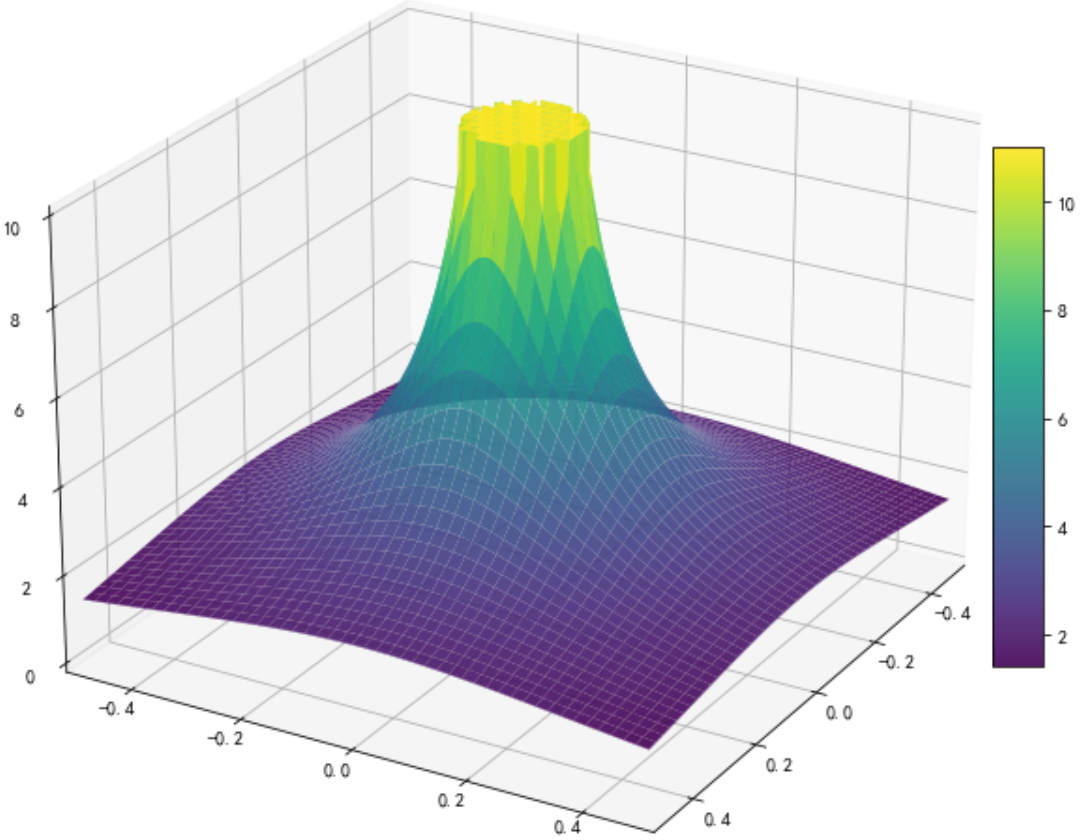
\includegraphics[width=0.7\textwidth]{tu/复变倒数1.png}
    \caption*{\texttt{函数}$z\mapsto\frac{1}{|z|}$\texttt{,用网格分析函数,用颜色表示函数值变化}}
\end{figure}

另外,复平面作为平面的特性与作为直线的数轴有本质区别,并对函数图像的分析有深刻影响。比如,如果实函数$f$在$0$处无定义,那么函数的图像必然是不连续的,例如在$0$处断为两截,我们无法讨论函数从$0$的一侧到另一侧的连续变化。然而,如果复变实函数$f$在$0$处无定义,函数的图像可以是一张在$0$处“缺了一点”的曲面,并不是断裂的,而是连通的。我们可以“绕过”无定义的$0$点,从$0$点一侧连到$0$点另一侧,讨论函数值的连续变化。

如果函数的值也是复数,那么我们甚至无法像复变实函数一样,用立体空间来呈现函数的性质了。这时我们要直观地理解函数的变化,就更加困难了。

如何直观呈现复变函数呢?常用的方法包括:
\begin{enumerate}
    \item 把自变量和函数值看作平面的向量,以自变量在复平面对应的点为起点,用函数值的模长和幅角对应的长短、方向的箭头来表现函数。这种方法来自物理学中的场论,把函数看成一种向量场。
    \item 把函数的值用两个实数表示,然后作为竖坐标,分别在两个立体空间中展现。常见的做法是分别展现函数值的模长和幅角。
    \item 把函数值的模长作为竖坐标,另外用颜色表示函数值的幅角,在立体空间展现函数的彩色图像。颜色变化表示函数幅角变化。
\end{enumerate}

\begin{et}
    研究复变函数$\displaystyle f: z \mapsto \frac{1}{z}$。
\end{et}

\begin{so}
    显然,$z = 0$时$f$无定义。对于非零复数$z$,记$z = a + b\imath $,计算$f(z)$:
    \begin{align*}
        f(z) &= \frac{1}{a + b\imath} = \frac{a - b\imath}{(a + b\imath)(a - b\imath)} \\
        &= \frac{a - b\imath}{a^2 + b^2} = \frac{a}{a^2 + b^2} - \frac{b}{a^2 + b^2} \imath
    \end{align*}
    只要$z \neq 0$,$f(z)$总有定义。

    我们也可以这样理解$f(z)$:
    $$ f(z) = \frac{\overline{z}}{\phantom{z}|z|^2}. $$
    从以上结果来看,$f(z)$的幅角和$\overline{z}$的幅角一样,是$z$的幅角的相反数。$f(z)$的模长是$z$的模的倒数。从函数图像来看,$f$除了在$0$处无定义,在其他地方很可能是连续乃至光滑的。论证这一点,需要定义复变函数的连续和光滑(可微)性质。
\end{so}

\begin{et}
    研究复变指数函数$\displaystyle f: z \mapsto \e^z$。
\end{et}

\begin{so}
    首先我们要定义$f$。$f$在$\mathbb{R}$上有定义。如何对一般的复数$z$定义$\e^z$呢?我们可以回顾定义实函数$x\mapsto \e^x$的过程。
    
    首先,我们在正整数集上定义了指数函数$x\mapsto a^x$,通过逆运算定义了有理数上的指数函数$x\mapsto a^x$。而由于有理数在数轴上密集分布,我们发现,可以用有理数来逼近任何实数。于是,对于任意实数$x$,我们把的$a^x$定义为有理数列$\{q_n\}$趋向$x$时$a^{q_n}$的极限。我们发现,这样的定义的实函数$x\mapsto a^x$很好,有优良的性质(连续、可微、光滑等)。通过研究指数函数和对数函数的性质,我们还发现了常数$\e$的特殊地位,于是定义了$x\mapsto \e^x$。

    要讨论$\e^z$,我们同样可以从定义$a^z$开始($a$是$1$以外的正数)。$z$是整数的时候,我们发现指数函数的根本性质是它满足:
    \begin{equation}
        \forall x, y \in \mathbb{N}, \quad a^{m + n} = a^m \cdot a^n. \label{4-6-0} 
    \end{equation}
    指数函数拓展到有理数乃至实数的过程,都是从这个性质出发。这个性质是指数函数的根本性质。及至复数范围,我们也希望指数函数保留这个性质。也就是说,对任意复数$z_1, z_2$:
    \begin{equation}
        \e^{z_1 + z_2} = \e^{z_1} \cdot \e^{z_2}. \label{4-6-1}
    \end{equation}
    为此我们可以假设:
    \begin{equation}
        \forall x, y \in \mathbb{R}, \quad a^{(x + y)\imath} = a^{x\imath} \cdot a^{y\imath}. \label{4-6-3}
    \end{equation}
    以及:
    \begin{equation}
        \forall x, y \in \mathbb{R}, \quad a^{x+y\imath} = a^x \cdot a^{y\imath},  \label{4-6-2}
    \end{equation}
    这样,由于$a^x$和$a^{y\imath}$都是复数,而复数的乘法满足交换律与结合律,于是:
    \begin{align*}
        \forall \; z_1 = x_1 + y_1\imath, \,&\; z_2 = x_2 + y_2\imath \; \in \mathbb{C}, \\
        a^{z_1 + z_2} &= a^{(x_1 + x_2) + (y_1 + y_2)\imath} = a^{(x_1 + x_2)} \cdot a^{(y_1 + y_2)\imath} \\
        &= a^{x_1} \cdot a^{x_2} \cdot a^{y_1\imath} \cdot a^{y_2\imath} \\
        &= a^{x_1} \cdot a^{y_1\imath} \cdot a^{x_2} \cdot a^{y_2\imath} \\
        &= a^{x_1 + y_1\imath} \cdot a^{x_2 + y_2\imath} \\
        &= a^{z_1} \cdot a^{z_2}.
    \end{align*}

    如何让这两个等式成立呢?对于\eqref{4-6-3},上一节我们已经验证过,如果以下假设成立:
    \begin{equation}
        \forall \; t\in\mathbb{R}, \quad \e^{\imath t} = \cos{t} + \imath \sin{t}. \label{4-6-4}
    \end{equation}
    那么\eqref{4-6-3}就成立。于是,我们把\eqref{4-6-3}转化为验证\eqref{4-6-4}。

    % 为了让\eqref{4-6-3}成立,我们比照指数函数的根本性质\eqref{4-6-0},假设:
    % \begin{equation}
    %     \forall \; t\in\mathbb{R}, \quad \e^{\imath t} = \cos{t} + \imath \sin{t}. \label{4-6-4}
    % \end{equation}
    % 事实上,如果关系\eqref{4-6-4}成立,那么可以用之前的方式推出:
    % $$ \forall \; q \in \mathbb{Q}, \quad a^{q\imath} = \left(a^{\imath}\right)^q. $$
    % 而$a^{\imath}$作为复数,可以写成:
    % $$a^{\imath} = r\cos{\theta} + r\imath\sin{\theta}, $$
    % 其中$r$和$\theta$分别是$a^{\imath}$的模长和幅角。于是:
    % $$ a^{q\imath} = \left(a^{\imath}\right)^q = r^q\cos{(q\theta)} + r^q\imath\sin{(q\theta)}. $$
    % 对于一般实数$t$,我们希望建立$a^{t\imath}$和$a^{q\imath}$的关系:
    % $$ \forall \; t\in\mathbb{R}, \quad a^{t\imath} = \lian{q\to t} a^{q\imath} = \lian{q\to t} \big(r^q\cos{(q\theta)} + r^q\sin{(q\theta)}\imath \big), $$
    % 事实上,如果我们假定以下关系成立:
    % \begin{equation}
    %     a^{t\imath} = r^t\cos{(t\theta)} + r^t\sin{(t\theta)}\imath = \lian{q\to t} \big(r^q\cos{(q\theta)} + r^q\sin{(q\theta)}\imath \big), \label{4-6-5}
    % \end{equation}
    % 这样,我们就可以验证关系\eqref{4-6-3}成立:
    % \begin{align*}
    %     \forall \; \{x_n\} ,\, \{y_n\} &\in \mathbb{Q}^{\mathbb{N}}, \\
    %     \{x_n\} \to x, &\; \{y_n\} \to y \; \in \mathbb{R}, \\
    %     a^{x\imath} \cdot a^{y\imath} &= \lian{n \to +\infty} \left(a^{\imath}\right)^{x_n} \cdot \lian{n \to +\infty} \left(a^{\imath}\right)^{y_n} = \lian{n \to +\infty} \left(a^{\imath}\right)^{(x_n + y_n)} \\
    %     &= a^{(x + y)\imath}.  \tag{$\{x_n + y_n\} \to x + y$}
    % \end{align*}

    等式\eqref{4-6-2}和\eqref{4-6-4}是否成立呢?后面的学习中,我们会进一步讨论这些问题。到时我们将发现$z \mapsto \e^z$的更多性质。
\end{so}

复变函数有着与实变函数截然不同的独特性质,但由于自变量是复数,比实变函数更抽象,难以直观理解。既然如此,我们要如何研究复变函数呢?我们将在后面的学习中逐步了解、掌握相关的工具,为分析、研究复变函数打下基础。

\begin{sk}
    \mbox{} \\
    \indent 1. 有没有可能用平面的曲线描述复变函数的性质?\\
    \indent 2. 说明:如果$\forall t\in\mathbb{R}, \;\,e^{it} = \cos{t} + \imath \sin{t}$成立,那么可以按照本节的方法定义任意复数$z$的指数$\e^z$。\\
    \indent 3. 是否能像从有理数的指数函数拓展到实变指数函数一样,把实变指数函数拓展到复变指数函数?\\
    \indent 4. 给定复数$z$,能否用级数定义$e^z$?这样定义的复变指数函数,是否满足$\e^x\cdot \e^y = \e^{x + y}$?
\end{sk}

% ############################## %
% \chapter{对称和群}
% 对称和群
% ############################## %

\chapter{无限与概率}

预测未来,是人类社会的重要活动。研究如何预测未来,处理不确定的事情,这样的理论称为概率论。我们已经学习过一些概率论的基本知识。

对于不确定的事情,我们把它所有可能的最终状态或局面看成一个集合,称为终集。集合中的每个元素称为事情的终态或结果。事件是终集的子集。“有什么事件”代表了我们对事情的认知,我们认知中的事件的集合称为知集。从集合的角度来看,知集是终集幂集的子集。知集满足:

\begin{enumerate}
    \item 空集属于知集;
    \item 如果集合$A$属于知集,那么$A$的补集也属于知集;
    \item 如果集合$A$和$B$属于知集,那么它们的交集和并集也属于知集。
\end{enumerate}

随着我们对事情认知逐渐深入,我们能讨论的事件越来越多,认识越来越细致,表现为终集和知集不断扩大。

预测随机事件时,我们主要关心事情有多大可能发生。我们用$0$到$1$之间的数表示某件事多么有可能发生,把这个数称为事件的概率。一件事越有可能发生,概率就越大。用数学的语言来说,概率是把集合映射到$0$与$1$之间的数的映射。我们一般把概率映射记为$\mathbb{P}$,它满足:

\begin{enumerate}
    \item 任意事件$A$的概率$\mathbb{P}(A)\in[0;1]$;
    \item 空集的概率是$0$,全集的概率是$1$;
    \item 如果$A\subseteq B$,那么$\mathbb{P}(A)\leqslant \mathbb{P}(B)$;
    \item 如果$A\cap B$是空集,那么$\mathbb{P}(A\cup B) = \mathbb{P}(A) + \mathbb{P}(B)$。
\end{enumerate}

如何讨论事件的概率?我们把知集中的基本事件的概率合起来看,称为概率的分布。只要知道了基本事件的概率,通过概率的性质,就能推出其他事件的概率。这样,我们就有了讨论不确定事件的基本工具。

不过,以前我们的讨论仅限于终集是有限集合的情况。如果终集是无限集合,会发生什么事呢?

\begin{ex}
    从自然数集合$\mathbb{N} = \{0,1,2,3,\cdots\}$中随机选取一个数,这个数是偶数的概率是多少?
\end{ex}

乍一看,这个问题的答案似乎是$\frac{1}{2}$,因为我们直觉上认为偶数和奇数“一样多”,甚至对于无限集合的势的讨论,也支持这个结论。但是,如果我们想用以上的工具来严格讨论这个问题,就会遇到困难。首先,我们要讨论的终集是$\mathbb{N}$,基本事件是任何自然数构成的单元集。而如何“随机选取一个数”,就涉及到概率分布的问题。

$\mathbb{N}$上的概率分布是怎样的呢?

\section{无限集合上的概率问题}

让我们回忆投骰子的实验。骰子的六面对应六个终态:$\{1,2,3,4,5,6\}$。如果我们假设投骰子的概率遵从均匀分布。每个基本事件的概率相等,都是$\frac{1}{6}$。于是“点数是偶数”的概率是:

$$ \mathbb{P}(\mbox{点数是偶数}) = \mathbb{P}(\{2,4,6\}) = \mathbb{P}(\{2\}) + \mathbb{P}(\{4\}) + \mathbb{P}(\{6\}) = \frac{1}{6} + \frac{1}{6} + \frac{1}{6} = \frac{1}{2}.$$

对终集为$\mathbb{N}$的情况,我们可以猜测:
\begin{align*}
    \mathbb{P}(\mbox{选的数是偶数}) = \mathbb{P}(\{0,2,4,6,\cdots\}) = \sum_{n=0}^{+\infty} \mathbb{P}(2n).
\end{align*}

要让这个式子成立,有两个必要的条件:首先,对任意$n$,我们能够合理地给出$\mathbb{P}(2n)$的值;其次,这无限个值可以求和。

如果我们不做多想,希望“在$\mathbb{N}$里随机选取一个数”也和投骰子一样,得到任何结果的概率都相等,也就是说对任意$n$,$\mathbb{P}(n)$都等于某个常数$c$。按概率的定义,$0\leqslant c\leqslant 1$。如果$c>0$,那么级数$\sum_{n=0}^{+\infty} \mathbb{P}(2n)$发散,无法求和。如果$c=0$,那么级数$\sum_{n=0}^{+\infty} \mathbb{P}(n)$的和为$0$,这说明全集的概率是$0$而不是$1$!

上面的矛盾情形让我们认识到,想当然地把有限的情况推广到无限是不行的。我们甚至无法轻松讨论“在$\mathbb{N}$里随机选取一个数”这种看来再简单不过的问题。那么困难到底出在哪里呢?

为了讨论无限集合上的概率问题,我们首先要定义“无限个概率相加”。使用级数的概念,我们可以处理可数个数相加。使用积合的概念,我们可以处理闭区间上的数“相加”。让我们先来处理可数个概率相加的问题。终集是有限集合时,我们这样规定:
\begin{quotation}
    如果$A\cap B$是空集,那么$\mathbb{P}(A\cup B) = \mathbb{P}(A) + \mathbb{P}(B)$。
\end{quotation}
这个规律可以轻松地推广到任意有限个集合:
\begin{quotation}
    \noindent 如果$A_1,A_2, \cdots, A_n$两两不相交,那么$\displaystyle\Pr{\bigcup_{i=1}^n A_i} = \sum_{i=1}^n \mathbb{P}(A_i).$
\end{quotation}
如果可数无限个集合,两两不相交,那么我们希望有这样的性质:
\begin{quotation}
    \noindent 如果$A_1,A_2, \cdots$两两不相交,那么$\displaystyle\Pr{\bigcup_{i=1}^{+\infty} A_i} = \sum_{i=1}^{+\infty} \mathbb{P}(A_i).$
\end{quotation}
我们把这个性质叫做概率的\textbf{可数可加}性质。

以上定义涉及到可数无穷个集合的并集。它是否有定义?是否属于知集?为此,我们要修改知集的基本性质,具体来说,我们要将知集的第三条性质改为:
\begin{quotation}
    \noindent 如果一族集合$\{A_i\}_{i\in\mathbb{N}}$都属于知集,那么它们的并集$\bigcup_{i\in\mathbb{N}} A_i$和交集$\bigcap_{i\in\mathbb{N}} A_i$也属于知集。
\end{quotation}
这样修改之后,配合概率的可数可加性质,我们就可以讨论可数无穷集合上的概率问题了。我们把终集$\Omega$、知集$\Sigma$和概率映射$\mathbb{P}$三者视为讨论任何概率问题的基础,将它们合称为\textbf{概率空间}。

\begin{ex}
    我们想知道正整数里有哪些素数,最容易想到的方法是“筛法”,即不断用已知最小的素数作为“筛子”,筛去它的倍数,剩余的数里最小的\footnote{除去$1$以外最小的。下同。}就是下一个素数。如果我们把全体正整数看作终集,把全体素数的集合看作事件,那么筛法的每一步操作都是在扩大知集。而最终把“是素数”这个事件纳入知集。

    设终集$\Omega$为全体正整数。我们从最小的素数$2$开始,首先筛去$2$的倍数。这时知集变为$\{\varnothing, \Omega, B_2, B_2^{\bu}\}$,有$2^{2^1} = 4$个元素。其中$B_2$是所有$2$的倍数的集合。
    $$B_2 = \{2,4,6,\cdots\}$$
    $B_2^{\bu}$中最小的是$3$,接下来筛去$3$的倍数。这时知集扩大为
    \begin{align*}
        \{\varnothing, \Omega, B_2, B_2^{\bu}, B_3, B_3^{\bu}, B_2\cup B_3, B_2\cap B_3, B_2\cup B_3^{\bu}, B_2\cap B_3^{\bu},\\
        B_2^{\bu}\cup B_3, B_2^{\bu}\cap B_3, B_2^{\bu}\cup B_3^{\bu}, B_2^{\bu}\cap B_3^{\bu}, \\ (B_2\cap B_3^{\bu})\cup(B_2^{\bu}\cap B_3), (B_2\cap B_3)\cup(B_2^{\bu}\cap B_3^{\bu})\}
    \end{align*}
    % $$\{\varnothing, \Omega, B_2, B_2^{\bu}, B_3, B_3^{\bu}, B_2\cup B_3, B_2\cap B_3, B_2\cup B_3^{\bu}, B_2\cap B_3^{\bu}, B_2^{\bu}\cup B_3, B_2^{\bu}\cap B_3, B_2^{\bu}\cup B_3^{\bu}, B_2^{\bu}\cap B_3^{\bu}\}$$
    一共$2^{2^2} = 16$个元素。其中$B_3= \{3,6,9,\cdots\}$是所有$3$的倍数的集合。所有被筛去的数的集合是$B_2\cup B_3$,剩余的数在$B_2^{\bu}\cap B_3^{\bu}$里,其中最小的是$5$。
    
    于是再筛去$5$的倍数集合$B_5$,知集继续扩大至$2^{2^3} = 256$个元素。依此类推,最终的知集里会有所有的“素数的倍数”的集合:$B_2, B_3, B_5, B_7, \cdots$。于是我们可以得到单个素数的集合:
    \begin{align*}
        \{2\} &= B_2 \setminus \left(B_3 \cup B_5 \cup B_7\cap\cdots\right) = B_2 \setminus \bigcup_{i=2}^{+\infty} B_{s_i} = B_2 \cap \left(\bigcup_{i=2}^{+\infty} B_{s_i} \right)^{\bu}, \\
        \{3\} &= B_3 \setminus \left(B_5 \cup B_7 \cup B_{11}\cap\cdots\right) = B_3 \setminus \bigcup_{i=3}^{+\infty} B_{s_i} = B_3 \cap \left(\bigcup_{i=3}^{+\infty} B_{s_i} \right)^{\bu}, \\
        \{5\} &= B_5 \setminus \left(B_7 \cup B_{11} \cup B_{13}\cap\cdots\right) = B_5 \setminus \bigcup_{i=4}^{+\infty} B_{s_i} = B_5 \cap \left(\bigcup_{i=4}^{+\infty} B_{s_i} \right)^{\bu}, \\
        &\vdots
    \end{align*}
    其中$s_i$是从小到大数起的第$i$个素数。于是全体素数的集合可以写为:
    $$ S = \{2\}\cup \{3\} \cup \{5\}\cup \{7\}\cup\cdots .$$
    它也在最终的知集里。
\end{ex}

从可数可加性可以推出以下的基本性质:
\begin{tm}
    给定递增事件序列$A_1\subseteq A_2\subseteq \cdots \subseteq A_n \subseteq A_{n+1} \subseteq \cdots$,那么
    $$ \Pr{\bigcup_{n=1}^{+\infty} A_n} = \lian{n\to+\infty} \mathbb{P}(A_n). $$
    给定递减事件序列$A_1\supseteq A_2\supseteq \cdots \supseteq A_n \supseteq A_{n+1} \supseteq \cdots$,那么
    $$ \Pr{\bigcap_{n=1}^{+\infty} A_n} = \lian{n\to+\infty} \mathbb{P}(A_n). $$
\end{tm}

\begin{proof}
    根据递增事件序列$A_1\subseteq A_2\subseteq \cdots \subseteq A_n \subseteq \cdots$定义新序列:
    $$ B_1 = A_1, \; B_2 = A_2\setminus A_1, \; B_3 = A_3\setminus A_2, \; \cdots$$
    $\{B_i\}_{i\in\mathbb{N}}$两两不相交,于是:
    $$ \Pr{\bigcup_{i=1}^{+\infty} B_i} = \sum_{i=1}^{+\infty} \mathbb{P}(B_i). $$
    而根据定义可以验证:
    \begin{align*}
        A_n = \bigcup_{i=1}^{n} B_i ,\quad \bigcup_{i=1}^{+\infty} A_i = \bigcup_{i=1}^{+\infty} B_i .
    \end{align*}
    于是:
    \begin{align*}
        \mathbb{P}(A_n) = \sum_{i=1}^{n} \mathbb{P}(B_i) , \quad
        \Pr{\bigcup_{i=1}^{+\infty} A_i} = \Pr{\bigcup_{i=1}^{+\infty} B_i} .
    \end{align*}
    因此:
    $$ \Pr{\bigcup_{i=1}^{+\infty} A_i} = \Pr{\bigcup_{i=1}^{+\infty} B_i} = \sum_{i=1}^{+\infty} \mathbb{P}(B_i) = \lian{n\to+\infty} \mathbb{P}(A_n). $$

    根据递减事件序列$A_1\supseteq A_2\supseteq \cdots \supseteq A_n \supseteq \cdots$定义新序列:
    $$ B_1 = A_1\setminus A_1 = \varnothing, \; B_2 = A_1\setminus A_2, \; B_3 = A_1\setminus A_3, \; \cdots$$

    $\{B_i\}_{i\in\mathbb{N}}$满足$B_1\subseteq B_2\subseteq \cdots \subseteq B_n \subseteq \cdots$,于是根据前面结论:
    $$ \Pr{\bigcup_{i=1}^{+\infty} B_i} = \lian{n\to+\infty}  \mathbb{P}(B_i). $$

    根据定义,$B_n$和$A_n$不相交,并集为$A_1$,所以
    $$ \mathbb{P}(B_n) + \mathbb{P}(A_n) = \mathbb{P}(A_1). $$

    集合$\bigcup_{i=1}^{+\infty} B_i$和$\bigcap_{i=1}^{+\infty} A_i$不相交,并集为$A_1$,所以
    $$ \Pr{\bigcup_{i=1}^{+\infty} B_i} + \Pr{\bigcap_{i=1}^{+\infty} A_i} = \mathbb{P}(A_1). $$

    因此:
    \begin{align*}
        &\mathbb{P}(A_1) - \Pr{\bigcap_{i=1}^{+\infty} A_i} = \Pr{\bigcup_{i=1}^{+\infty} B_i} = \lian{n\to+\infty}  \mathbb{P}(B_n) \\
        =\;& \lian{n\to+\infty} \left( \mathbb{P}(A_1) - \mathbb{P}(A_n) \right) = \mathbb{P}(A_1) - \lian{n\to+\infty} \mathbb{P}(A_n).
    \end{align*}
    
    也就是说:
    $$ \Pr{\bigcap_{i=1}^{+\infty} A_i} = \lian{n\to+\infty} \mathbb{P}(A_n). $$
\end{proof}

这两个基本性质可以看作“子集概率不大于母集”延伸到可数无穷的情形。从中又可以推出“并集概率不大于概率之和”的延伸:
\begin{tm}
    给定事件序列$\{A_i\}_{i\in\mathbb{N}}$,则它们并集的概率满足:
    $$ \Pr{\bigcup_{i=1}^{+\infty} A_i} \leqslant \sum_{i=1}^{+\infty} \mathbb{P}(A_i). $$
\end{tm}

\begin{proof}
    可数可加性质说明,如果$\{A_i\}_{i\in\mathbb{N}}$两两不相交,那么不等号可以变为等号。对于一般的情况,我们可以构造两两不相交的事件序列:
    $$ B_1 = A_1, \; B_2 = A_2\setminus A_1, \; B_3 = A_3\setminus (A_1 \cup A_2), \; B_4 = A_4\setminus (A_1 \cup A_2 \cup A_3), \; \cdots$$
    可以验证$\{B_i\}_{i\in\mathbb{N}}$两两不相交,且$\bigcup_{i=1}^{+\infty} A_i = \bigcup_{i=1}^{+\infty} B_i$,于是:
    $$  \Pr{\bigcup_{i=1}^{+\infty} A_i} = \Pr{\bigcup_{i=1}^{+\infty} B_i} = \sum_{i=1}^{+\infty} \mathbb{P}(B_i). $$
    而任意$B_i$总是$A_i$的子集,所以$\mathbb{P}(B_i)\leqslant \mathbb{P}(A_i)$。因此:
    $$ \Pr{\bigcup_{i=1}^{+\infty} A_i} = \sum_{i=1}^{+\infty} \mathbb{P}(B_i) \leqslant \sum_{i=1}^{+\infty} \mathbb{P}(A_i). $$
\end{proof}

\section{可数无限集合上的分布}

既然以$\mathbb{N}$为终集的概率空间无法均匀分布,那么可以有怎样的分布呢?

从前面的讨论,我们发现,讨论$\mathbb{N}$上的概率分布$\mathbb{P}$的实质是讨论通项非负的收敛无穷级数:
$$ \sum_{n=1}^{+\infty} \mathbb{P}(\{k\}) = 1. $$
所以,无穷级数的性质会反映为$\mathbb{P}$的性质。比如,我们知道要使级数收敛,通项必须收敛到$0$,而且要收敛得足够快。因此,任何以$\mathbb{N}$为终集的概率分布,必然有“概率随着数增大而趋于$0$”。

反过来,从任何收敛的正项级数出发,是否都可以构造概率分布进而构造概率空间呢?答案是肯定的。
\begin{tm}{\textbf{概率空间存在定理}}
    设有正项级数:
    $$ \sum_{n=1}^{+\infty} a_n = S > 0,$$
    那么它对应一个$\mathbb{N}$上的概率空间。即有概率分布$\mathbb{P}$使得:
    $$ \forall n\in\mathbb{N},\quad \mathbb{P}(\{n\}) = \frac{a_n}{S}.$$
    它对应的终集是$\mathbb{N}$,知集是其幂集$\Omega = 2^{\mathbb{N}}$。
\end{tm}

\begin{proof}
    我们要证明的是映射:
    $$ \forall n\in\mathbb{N},\quad \mathbb{P}(\{n\}) = \frac{a_n}{S}.$$
    满足作为概率分布的基本性质:
    \begin{enumerate}
        \item $\forall A \in \Omega$,$\Pr{A} \geqslant 0.$
        \item $\Pr{\Omega} = 1.$
        \item $\forall A \subseteq B$,$\Pr{A} \leqslant \Pr{B}.$
        \item 给定可数个两两不相交的集合$\{A_i\}_{i\in \mathbb{N}} $,
        $$ \Pr{\bigcup_{i\in \mathbb{N}} A_i} = \sum_{i\in \mathbb{N}} \Pr{A_i}. $$
    \end{enumerate}

    记$b_n = \frac{a_n}{S}$,则级数$\sum b_n$是和为$1$的正项级数。根据映射$\mathbb{P}$的定义和可求和数族的性质,任意事件$\mathbb{N}$的子集对应的概率,都可以定义为基本事件族的概率的和:
    $$ \forall A \in \Omega, \quad \Pr{A} = \sum_{i\in A} \Pr{\{n\}} = \sum_{i\in A} b_n. $$
    即$\mathbb{P}$对基本事件可数可加。

    据此可以证明前面三个基本性质。首先,由于$\sum b_n$是正项级数,
    $$\forall A \in \Omega ,\quad \Pr{A} = \sum_{i\in A} b_n \geqslant 0.$$
    
    其次,$\sum b_n$的和为$1$,这说明
    $$\Pr{\Omega} = \sum_{n\in \mathbb{N}} b_n = 1.$$

    再者,对于$A \subseteq B$,由于$\sum_{i\in A} b_i$和$\sum_{i\in B} b_i$都是可求和数族,根据可求和数组的基本性质,
    $$\Pr{A} = \sum_{i\in A} b_i \leqslant \sum_{i\in B} b_i = \Pr{B}.$$
    
    最后我们来证明这样的定义下,任意事件的概率都可数可加。

    给定可数个两两不相交的集合$\{A_i\}_{i\in \mathbb{N}} $,我们要证明:
    $$ \Pr{\bigcup_{i\in \mathbb{N}} A_i} = \sum_{i\in \mathbb{N}} \Pr{A_i}. $$
    记$B = \bigcup_{i\in \mathbb{N}} A_i$,由于集合$A_i$两两不相交,$B$中任何一个元素恰好属于某个$A_i$,没有重复没有遗漏。因此,
    $$ \Pr{B} = \sum_{k\in B} b_k = \sum_{n\in \mathbb{N}} \sum_{i\in A_n} b_i = \sum_{i\in \mathbb{N}} \Pr{A_i}. $$

\end{proof}

概率空间存在定理告诉我们,对$\mathbb{N}$上的概率空间来说,分布的具体“长相”是最重要的。知道了概率分布,自然能造出对应的概率空间。一般的可数集合与$\mathbb{N}$等势,因此也可以用以上的方法构造对应的概率空间。

\section{离散随机变量的分布}

以上提到的是概率空间中的分布。概率空间中的随机变量也遵从某种分布。设$X$是某概率空间$\Omega, \Sigma, \mathbb{P}$上的随机变量,它将$\Omega$中的元素映射到集合$S$中。如果$S$是有限或可数无限集合,就说随机变量$X$是\textbf{离散}的。我们已经学习过取值在有限集合上的离散随机变量。下面来看取值在可数无限集合上的随机变量。

我们说随机变量给每个基本事件对应一个$0$与$1$之间的数,称为它的概率。另一种方式是直接讨论随机变量每个取值的概率。随机变量遵从的分布

\begin{ex}
    考虑不断掷硬币的独立实验,掷出正面就停止。每次掷硬币都是一次独立事件,掷出正面的概率都是$0<p<1$,反面的概率都是$1-p$。那么掷第$n$次时首次出现正面的概率是怎样的?
\end{ex}

\begin{so}
    对任意正整数$n$,设掷硬币第$n$次时首次出现正面,那么前$n-1$次都是反面。于是随机变量“首次出现正面的次数”$X$遵从的分布为\footnote{这里的$\Pr{X=n}$表示$\Pr{\{s\in\mathbb{N}\,| \, X(s) = n\}}$。下同。}:
    $$ \Pr{X=n} = (1 - p)^{n-1} p.$$
    因此我们讨论的是以下的分布:
    $$ \forall n \in \mathbb{N}, \quad \Pr{X=n} = (1 - p)^{n-1} p. $$
    对所有的$n$求和:
    \begin{align*}
        \sum_{n=1}^{+\infty} \Pr{X=n} &= \sum_{n=1}^{+\infty}(1 - p)^{n-1} p = p\cdot \sum_{n=1}^{+\infty}(1 - p)^{n-1} \\
        &= p \cdot \frac{1}{1 - (1 - p)} = 1.
    \end{align*}
    严格来说,这是正整数集合$\mathbb{Z}^+$上的分布。它的“通项”是一个无穷等比数列。所以我们称它为\textbf{等比分布}。
\end{so}

等比分布的公比为$1 - p$,所以它对应一个递缩等比数列。“首项”$\Pr{X=n}$是最大的,其后不断变小。我们还可以计算“前$n$次都不出现正面”的概率:
\begin{align*}
    \Pr{\mbox{前}n\mbox{次都不出现正面}} &= \sum_{k=n+1}^{+\infty} \Pr{X=k} = \sum_{k=n+1}^{+\infty} (1 - p)^{k-1}p\\ 
    &= p(1 - p)^{n}\cdot \sum_{k=0}^{+\infty} (1 - p)^k = p(1 - p)^{n}\cdot \frac{1}{1 - (1 - p)} \\
    &= (1 - p)^{n}.
\end{align*}

另一个例子和二项分布有关。

\begin{ex}
    某县今年平均每天有10名婴儿出生,估计下一年的婴儿出生数量大致不变。那么,明年每天出生的婴儿数量如何分布?
\end{ex}

\begin{so}
    为了简化问题,方便讨论,我们假设“婴儿出生”这件事是瞬时的,比如我们认定剪断脐带的瞬间作为“婴儿出生”的时刻。此外,“婴儿出生”的事件在一年、一天中“均匀发生”,即在任意很短的时间段内,事件发生的概率和时间段长度成正比。最后,假设足够短时间段内发生多于一次“婴儿出生”(包括多胞胎)的概率,相比发生至多一次的概率可以忽略。

    在这样的假设下,如果我们把一天的时间$T$分为很多小时间段,比如分成$n$个$\frac{T}{n}$长的时间段,那么当$n$足够大的时候,每段时间内要么有一次“婴儿出生”,要么没有。这是一个$n$次二项分布。设其正面概率为$p_n$,那么一天的$n$个时间段里发生$k$次事件的概率为:
    $$ \Pr{X = k} = \bino{n}{k} p_n^k(1 - p_n)^{n-k}. $$
    其中$X$是“一天内婴儿出生数量”这个随机变量。
    考虑$n$趋于无穷的情况。由于我们假设事件发生的概率和时间段长度成正比,因此$np_n$对应一天的总长度,是一个与$n$无关的常数。记$a = np_n$,于是$p_n = \frac{a}{n}$,而上面的概率可以写为:
    \begin{align*}
        \Pr{X = k} &= \frac{n!}{k!(n - k)!} \frac{a^k}{n^k}\left(1 - \frac{a}{n}\right)^{n-k} \\
        &= \frac{a^k}{k!} \frac{n(n - 1)\cdots(n - k)}{n^k}\left(1 - \frac{a}{n}\right)^{n-k} \\
        &= \frac{a^k}{k!} \frac{\left(1 - \frac{0}{n}\right) \left(1 - \frac{1}{n}\right)\cdots\left(1 - \frac{k-1}{n}\right)}{\left(1 - \frac{a}{n}\right)^k}\left(1 - \frac{a}{n}\right)^{n} 
    \end{align*}
    对给定的$k$,当$n$趋于无穷时,前面的$\left(1 - \frac{i}{n}\right)$全趋于$1$,而后面的$\left(1 - \frac{a}{n}\right)^{n}$趋于$\e^{-a}$。于是整体来说,以上概率趋于:
    $$ \frac{a^k\e^{-a}}{k!}. $$
    于是我们可以认为\footnote{以上的假设和推导都有不严谨之处,这里不作讨论,仅作思路的演示。有兴趣的读者可以在专门学习概率论的时候做严格的推导。}:
    $$ \forall k \in \mathbb{N}, \quad \Pr{X = k} = \frac{a^k\e^{-a}}{k!}. $$
    这是一个$\mathbb{N}$上的概率分布。我们可以验证,所有概率都非负,它们的和为$1$:
    \begin{align*}
        \sum_{k=0}^{+\infty} \Pr{X = k} &= \sum_{k=0}^{+\infty} \frac{a^k\e^{-a}}{k!} \\
        &= \e^{-a} \cdot \sum_{k=0}^{+\infty} \frac{a^k}{k!} = \e^{-a} \cdot \e^{a} \\
        &= 1.
    \end{align*}
    这个分布第$k$项的形式很像指数函数展开式的第$k$项,所以叫做\textbf{指数分布}。

    % 我们来求随机变量$X$的期望:
    % \begin{align*}
    %     \mathbb{E}(X) &= \sum_{i=0}^{+\infty} k \Pr{X = k} \\
    %     &= \sum_{i=0}^{+\infty} k \frac{a^k\e^{-a}}{k!} = \sum_{i=1}^{+\infty} k \frac{a^k\e^{-a}}{k!} \\
    %     &= a \sum_{i=1}^{+\infty} \frac{a^{k-1}\e^{-a}}{(k - 1)!} = a \sum_{i=0}^{+\infty} \frac{a^k\e^{-a}}{k!} \\
    %     &= a.
    % \end{align*}
    % 也就是说,$X$的期望是$a$,符合我们的假设。我们把$a$称为指数分布的系数。于是该县明年每天出生的婴儿数遵从系数$a=10$的指数分布。
\end{so}



\begin{sk}
    \mbox{} \\
    \indent 1. 指数分布的例子里,为什么可以假设足够短时间内发生多于一次事件的概率,相比发生至多一次的概率,可以忽略?\\
    % \indent 2. 
\end{sk}
% 讨论实变函数中的可测函数

% 引入勒贝格积分

% \section{可数无限概率空间}

% 定义可数个元素构成的事件集合和概率空间。定义事件的概率。

% ----------------- 第六册 --------------

% \chapter{离散随机变量}

% \section{随机变量的性质}

% \section{正态分布}

% \section{大数定律}

% \section{中心极限定理}

% %%%%%%%%%%%%%%%%%%%%%%%%%% %
%                            %
%          APPENDIX          %
%                            %
% %%%%%%%%%%%%%%%%%%%%%%%%%% %

\begin{appendix}

\chapter{复数}

\section{复数与方程}

\begin{tm}{\textbf{代数基本定理}}
    \mbox{} \\
    次数大于零的复系数整式至少有一个复数根。
\end{tm}

\begin{proof}
    % Oswaldo Rio Branco de Oliveira, The Fundamental Theorem of Algebra: An Elementary and Direct Proof. Math Intelligencer 33, 1–2 (2011). https://doi.org/10.1007/s00283-011-9199-2
    设$P$是次数大于零的整式:
    $$ P(x) = a_0 + a_1 x + \cdots + a_n x^n.$$
    其中$a_0, a_1, \cdots , a_n$是复数,$a_n \neq 0$。
    我们要证明:有复数$z_0\in\mathbb{C}$,使得$P(z_0) = 0$。

    对整式$P$取模:
    $$ |P(x)| = |a_0 + a_1 x + \cdots + a_n x^n|. $$
    根据三角形边长的关系,我们知道:
    $$ |P(x)| \geqslant |a_n| |x|^n - |a_0| - |a_1||x| - \cdots - |a_{n-1}| |x|^{n-1}. $$
    因此,当$|x|$趋于正无穷时,$|P(x)|$趋于正无穷。因此,根据整式函数的连续性,$x\mapsto |P(x)|$在定义域内取到最小值\footnote{这个结论将在后面的学习中学到。本书不作证明。}。

    设$z_0$是取最小值的点。我们希望证明:$|P(z_0)| = 0$。
    
    通过平移的方法,我们可以假设$z_0 = 0$。于是$P(z_0) = a_0$。我们考虑以$z_0$为圆心的单位圆:
    $$ S^1 = \{\omega\in\mathbb{C} \, | \, |\omega| = 1\}$$

    按$z_0$定义,我们有这样的关系:
    $$ \forall \; r > 0, \; \omega \in S^1,\quad  |P(r\omega)|^2 - |P(z_0)|^2 \geqslant 0. $$ 

    设$k$是$a_1, a_2, \cdots, a_n$等系数中不等于零的系数里下标最小的,那么$1\leqslant k < n$。
    我们可以将$P$表示成:
    $$ P(x) = a_0 + x^k Q(x). $$
    其中$Q$是次数为$n - k$的整式。按定义,$Q(0) = a_k \neq 0$。

    于是上面的不等关系变为:
    \begin{align*}
        0 &\leqslant |a_0 + r^k \omega^k Q(r\omega)|^2 - |a_0|^2 \\
          &= 2r^k \Re(\overline{a_0} \omega^k Q(r\omega)) + r^{2k}|Q(r\omega)|^2 
    \end{align*}
    $k\geqslant 1$,于是当$r$趋于$0$的时候,$r^{2k}$是$r^k$的高阶无穷小。因此为了上式总成立,需要有
    $$ \forall \; r > 0,\; \omega \in S^1,\quad \Re(\overline{a_0} \omega^k Q(r\omega)) \geqslant 0. $$
    令$r$趋于$0$,就有
    $$ \forall \; \omega \in S^1,\quad \Re(\omega^k\overline{a_0} Q(0)) \geqslant 0. $$

    记$\alpha = \overline{a_0} Q(0)$。$\alpha \in\mathbb{C}$是定值。
    前面不等式说明,当$\omega$在单位圆$S^1$上取值时,$\omega^k \alpha$的实部总大于等于零。
    我们尝试用$S^1$上的不同$\omega$代入上面不等式,得到$\alpha$的限制条件。

    从平面向量的角度来看,$\omega^k \alpha$的实部就是$\omega^k$和$\overline{\alpha}$的点积。它的实部大于等于零,
    就是说$\omega^k$和$\overline{\alpha}$张成的角度不超过直角。
    比如,$\omega^k$指向北,$\overline{\alpha}$就要指向东北或西北,不能指向东南或西南。

    然而,$\omega$沿着$S^1$转动的时候,$\omega^k$可以指向任意方向,这就对$\alpha$的方向提出了严格的要求。

    将$\omega = 1$代入,这时$\omega^k = 1$,于是$\omega^k \alpha$的实部就是$\alpha$的实部:$\Re(\alpha) \geqslant 0$。

    再令$\omega$为$\omega^k = -1$的解,于是:$\Re(\alpha) \leqslant 0$。%,设$\omega$是$z^{2^j} = -1$

    综上可知$\alpha$的实部为零。

    类似地,令$\omega$为$\omega^k = \pm \imath$的解,将其代入,%设$\omega$是$z^{2^j} = \pm \imath$的解,将其代入,
    就得到$\Im(\alpha) \geqslant 0$,$\Im(\alpha) \leqslant 0$。
    于是,可知$\alpha$的虚部为零。

    这说明$\alpha = 0$。而$\alpha = \overline{a_0} Q(0)$,但按定义$Q(0)\neq 0$,
    所以$\overline{a_0} = 0$,也就是说$a_0 = 0$。换句话说:
    $$ P(z_0) = P(0) = a_0 = 0. $$
    这样,我们就证明了$P$有复数根。

    最后说明以上的$\omega$总存在。首先,我们可以简单地用极坐标来推得这些解。比如$\omega^k = -1$的一个解是$\left(1, \frac{\pi}{k}\right)$。
    
    为了更明确地给出这些解,我们可以记$k = 2^j m$,其中$j$是自然数,$m$是奇数。我们知道$z^2 = a + b\imath$的解可以
    经过开方和四则运算得到。因此,重复$j$次,可以求出$z^{2^j} = \pm \imath$的解,记为$\jmath_+$和$\jmath_-$。
    于是
    $$\jmath_+^k = \left(\jmath_+^{2^j}\right)^m = \imath^m, \quad \jmath_-^k = \left(\jmath_+^{2^j}\right)^m = (-\imath)^m = -\imath^m.$$
    $m$是奇数,这说明两者$\imath^m$和$-\imath^m$一个是$\imath$,一个是$-\imath$,于是$\jmath_+$和$\jmath_-$分别是$\omega^k = \pm \imath$的解。

\end{proof}

从代数基本定理出发,立刻可以得到以下结论:

\begin{tm}{\textbf{整式有根定理}}
    \mbox{} \\
    \indent 一元复系数整式所有的根都在复数域里。$n$次复系数整式$P$可以写成:
    $$ P(x) = a(x - z_1)(x - z_2)\cdots(x - z_n).$$
    其中$a, z_1, z_2,\cdots, z_n$是复数,$a\neq 0$。   
\end{tm}

\begin{proof}
    使用归纳法。命题$\mathbb{P}(n)$:
    次数为$n$的一元复系数整式的所有根都在复数域里,$n$次复系数整式$P$可以写成:
    $$ P(x) = a(x - z_1)(x - z_2)\cdots(x - z_n).$$
    其中$a, z_1, z_2,\cdots, z_n$是复数,$a\neq 0$。 

    命题$\mathbb{P}(0)$、$\mathbb{P}(1)$显然成立\footnote{常数整式没有根,即根的集合是空集,因此在“根的集合是复数域子集”的意义上来说是成立的。或者说,“只要有根,就在复数域里”。}。假设命题对小于$n$的正整数成立,
    下面证明命题$\mathbb{P}(n)$成立。

    设有次数为$n$的一元复系数整式$P$,根据代数基本定理,它在复数域里至少有一个根,记为$z_n$。则通过带余除法可知:
    $$ P(x) = (x - z_n)Q(x).$$
    其中$Q$是次数为$n-1$的复系数整式。因此根据归纳假设,$Q$的所有根都在复数域里,$Q$可以写成:
    $$ Q(x) = a(x - z_1)(x - z_2)\cdots(x - z_{n-1})$$
    其中$a, z_1, z_2,\cdots, z_{n-1}$是复数,$a\neq 0$。因此,
    \begin{align*} 
        P(x) &= (x - z_n)Q(x) \\
        &= a(x - z_1)(x - z_2)\cdots(x - z_{n-1})(x - z_n).
    \end{align*}
    其中$a, z_1, z_2,\cdots, z_n$是复数,$a\neq 0$。于是命题$\mathbb{P}(n)$成立。

    综上所述,任何一元复系数整式所有的根都在复数域里。$n$次复系数整式$P$可以写成:
    $$ P(x) = a(x - z_1)(x - z_2)\cdots(x - z_n).$$
    其中$a, z_1, z_2,\cdots, z_n$是复数,$a\neq 0$。 

\end{proof}

既然复系数整式所有的根都在复数域里,实系数整式的系数都是实数,也是复数,因此实系数整式所有的根也都在复数域里。
同样,有理系数、整系数的整式,所有的根也都在复数域里。可以说,复数域里可以找到所有整式方程的根。所有的代数数都在复数域里。
因此,我们说复数域是\textbf{代数封闭}的。

不过,复数里并不是只有代数数。很多复数不是任何整式方程的根。换句话说,对于整式方程来说,复数域“太大了”。
如果复数$z$不是任何整式方程的根,就说它是\textbf{超越数}。数学家已经证明,圆周率$\pi$和自然指数的底$e$都是超越数。

有了整式有根定理,我们可以更进一步研究整式方程。

设$P$是一元$n$次实系数整式方程。如果$n$是奇数,那么通过分析实函数$x\mapsto P(x)$的性质,可以证明它至少有一个实数根。

考虑整式函数:
$$P: x\mapsto a_0 + a_1 x + \cdots + a_n x^n$$
实数$x$趋于正负无穷时,$x^n$是其他项的高阶无穷大。因此,$x$足够大时,$P(x)$的正负由$a_nx^n$这一项决定。

$n$是奇数时,$x^n$的正负随着$x$的正负变化,因此$a_nx^n$要么在负无穷处趋于负无穷,在正无穷处趋于正无穷;
要么反过来,在负无穷处趋于负无穷,在正无穷处趋于正无穷。对任何一种情况,都可以找到$a<0<b$,使得$P(a)$和$P(b)$异号。
这说明$P$在区间$(a;b)$上有根。
我们可以把$P$写成:
$$ P(x) = (x - x_n)Q(x).$$
其中$x_n$是$P$的根,$Q$是偶数次的整式。

实系数整式$P$的次数$n$是偶数时,不一定有实数根。但根据整式有根定理,它有复数根,可以写成:
$$ P(x) = a(x - z_1)(x - z_2)\cdots(x - z_n).$$
其中$a, z_1, z_2,\cdots, z_n$是复数,$a\neq 0$。

$a$就是$P$的最高次项,因此是实数。考虑任意实数$x$,$P(x)$也是实数,因此等于它的共轭。取共轭,可以发现:
$$ \overline{a}(\overline{x} - \overline{z_1})(\overline{x} - \overline{z_2})\cdots(\overline{x} - \overline{z_n}) = \overline{P(x)} = P(x).$$
其中实数的共轭等于自身,于是
\begin{align*}
    P(x) &= \overline{a}(\overline{x} - \overline{z_1})(\overline{x} - \overline{z_2})\cdots(\overline{x} - \overline{z_n}) \\
    &= a(x - \overline{z_1})(x - \overline{z_2})\cdots(x - \overline{z_n}). 
\end{align*}
这说明$P$的根的共轭仍然是它的根。
\begin{tm}{\textbf{虚根成对定理}}
    如果复数$z$是实系数整式$P$的根,那么它的共轭$\overline{z}$也是$P$的根。
\end{tm}
虚根成对定理说明,偶数次实系数整式$P$的根要么是实数,要么是成对出现的,每对根互为共轭\footnote{详细证明留作习题2。}。
  
如果$P$的根$z_i$不是实数,那么二次式$(x - z_i)(x - \overline{z_i})$是$P$的因式。将其展开,可以得到:
\begin{align*}
    (x - z_i)(x - \overline{z_i}) &= x^2 - (z_i + \overline{z_i}) + z_i\cdot\overline{z_i} \\
    &= x^2 - 2\Re(z_i)x + |z_i|^2
\end{align*}

设$P$的根中有$m$对共轭的实数,其余的$n-2m$个根是实数根。那么$P$可以写成:
$$ P(x) = aR(x)I(x).$$
其中$R(x)$是$n-2m$次整式,可以写成一次式的乘积:
$$ R(x) = (x - x_1)(x - x_2)\cdots(x - x_{n-2m}), $$
其中$x_1, x_2, \cdots, x_{n-2m}$是实数。$I(x)$是$2m$次整式,可以写成实系数二次式的乘积:
$$ I(x) = (x^2 - 2\Re(z_1)x + |z_1|^2) \cdots (x^2 - 2\Re(z_m)x + |z_m|^2)$$

综上所述,任何一元实系数整式$P$总可以写成实系数一次式和无实数根的实系数二次式的乘积。
$$ P(x) = a\prod_{i=1}^{n-2m}(x - x_i) \prod_{i=1}^m (x^2 - b_ix + c_i). $$

\begin{xt}
    \mbox{} \\
    \indent 1. 直观地说明代数基本定理的证明思路。\\
    \indent 2. 设$P$是次数大于零的实系数整式。\\
    \indent 2.1. 说明$P$的根的共轭仍然是它的根。\\
    \indent 2.2. 设$z$是$P$的根,且$z$不是实数,证明:
    $$ P(x) = (x - z)(x - \overline{z}) Q(x),$$
    其中$Q$是实系数整式。\\
    \indent 2.3. 用归纳法证明:偶数次实系数整式$P$的根要么是实数,要么是成对出现的,每对根互为共轭。\\
    \indent 3. 设$n$为正整数,考虑多项式:
    $$ P_n(x) = x^n + x^{n-1} + \cdots+ x + 1 . $$
    \indent 3.1. 求多项式$P_n$的所有根。\\
    \indent 3.2. 设$k$是正整数,求$\sum_{i=0}^{n-1}\cos{\left(\frac{2ki\pi}{n}\right)}$的值。\\
    \indent 4. 设$a$为实数,考虑多项式$P_a(x) = x^3 - 3x + a$。\\
    \indent 4.1. 画出$P_a$的曲线,用$a$表示它的极大值、极小值点。$a$变化时,曲线如何变化?\\
    \indent 4.2. $a$取什么值的时候,$P_a$有重根?在此情况下,求出它所有的根。\\
    \indent 5. 设$n$为正整数。给定$n+1$个两两不同的实数$x_0, x_1, \cdots, x_n$,以及$n+1$个实数$y_0, y_1, \cdots, y_n$。\\
    \indent 5.1. 考虑多项式:
    $$ L_i(x) = \prod_{k\neq i}\frac{(x - x_i)}{(x_k - x_i)}.$$
    $L_i$是以除$x_i$以外的$n$个数作为根的多项式。考虑多项式:
    $$ P(x) = \sum_{i=0}^n y_i L_i(x).$$
    证明:对任意$0\leqslant i\leqslant n$,$P(x_i) = y_i$。我们称这样的多项式$P$为\textbf{插值多项式}。$P$刚好穿过$n+1$个指定的点:$(x_0,\,\,y_0)$、$(x_1,\,\,y_1)$,……$(x_n,\,\,y_n)$。\\
    \indent 5.2. 证明:上一问中,次数不超过$n$的插值多项式$P$是唯一的。\\
    \indent 5.3. 证明$\left(L_i\right)_{0\leqslant i \leqslant n}$是$\mathbb{R}_n[x]$的基底。\\
    \indent 5.4. 设有复系数整式$P$。如果对任意有理数$x$,$P(x)$都是有理数,证明:$P$的系数都是有理数。\\
    \indent 6. 整式$P$满足:$P(0)=0$,且$P(x^2 + 1) = P(x)^2 + 1$。\\
    \indent 6.1. 求数列$\{u_n\}_{n\in\mathbb{N}}$,使得$P(u_n) = u_n$总成立。\\
    \indent 6.2. 求所有满足条件的整式$P$\footnote{提示:考虑整式$Q(x) = P(x) - x$。}。\\
    \indent 7. 考虑整式序列$\{T_n\}_{n\in\mathbb{N}}$:$T_0 = 1$,$T_1 = x$,且:
    $$ \forall n\in\mathbb{N}, \quad T_{n+2}(x) = 2xT_{n+1}(x) - T_n(x).$$
    \indent 7.1. 写出$T_2$和$T_3$的具体形式。\\
    \indent 7.2. 证明:$T_n$是$n$次整式,最高次项系数为$2^{n-1}$。\\
    \indent 7.3. 证明:对任意实数$\theta$,任意自然数$n$,
    $$ T_n(\cos{\theta}) = \cos{(n\theta)}.$$
    我们称$T_n$为$\boldsymbol{n}$\textbf{次余弦多项式}。\\
    \indent 7.4. 证明:$T_n$的所有根在区间$(-1;1)$上,且两两不同。\\
    \indent 7.5. 证明:对任意自然数$n$,可以找到整式$U_n$,使得:
    $$ \forall \theta \in \mathbb{R}, \quad U_n(\cos{\theta}) \sin{\theta} = \sin{((n+1)\theta)}. $$
    并说明$U_n$和$T_n$的关系。我们称$U_n$为$\boldsymbol{n}$\textbf{次正弦多项式}。\\
    \indent 7.6. 证明:
    $$ \forall n\in\mathbb{N},\,\, x\in\mathbb{R}, \;\; (1 - x^2)\partial^2 T_n(x) - x\partial T_n(x) + n^2 T_n(x) = 0.$$
    \indent 8. 设$n$为正整数,$P$为$n$次整式,最高次项系数为$a$。\\
    \indent 8.1. 求余弦多项式$T_n$在区间$[-1;1]$上绝对值的最大值,以及相应的极值点。\\
    \indent 8.2. 记$b$为集合$\{|P(x)| \, | \, x\in[-1;1]\}$的上确界。
    证明:$b \geqslant \frac{|a|}{2^{n-1}}$\footnote{提示:考虑$Q(x) = 2^{n-1}P(x) - aT_n(x)$在使$T_n$绝对值最大的点的值。}。\\
    \indent 8.3. 以上结论说明了余弦多项式的什么特性?你认为这种特性可以有什么用途?
\end{xt}

\section{复数与不等式}

我们学习过有理数和实数的不等式。有理数和实数的基本不等关系之一是“负负得正”,即两个负数的积是正数。从这一点出发可以得到很多不等式。比如重要的不等式:任何数的平方大于等于零。

对复数来说,这个不等式不再成立。因此,依赖这个不等式的很多不等式,在复数范围内也要重新考虑。其中包括内积不等式:
$$ \forall a_1, a_2, \cdots, a_n, b_1, b_2, \cdots, b_n \in \mathbb{R}, \quad \left(\sum_{i=1}^n a_i^2\right)\cdot\left(\sum_{i=1}^n b_i^2\right)\geqslant \left(\sum_{i=1}^n a_ib_i\right)^2.$$

回顾内积不等式的证明,我们发现,内积不等式也建立在“平方不小于零”上。
对于多元有序数组$(a_1, a_2, \cdots, a_n)$和$(b_1, b_2, \cdots, b_n)$,
\begin{align*}
    &(a_1^2 + a_2^2 + \cdots + a_n^2)(b_1^2 + b_2^2 + \cdots + b_n^2)  \\
    =\,\,& (a_1b_1 + a_2b_2 + \cdots + a_nb_n)^2 + \frac{1}{2}\sum_{i=1}^n\sum_{j=1}^n(a_ib_j - a_jb_i)^2  \\
    \geqslant\,\,& (a_1b_1 + a_2b_2 + \cdots + a_nb_n)^2  
\end{align*}
复数是否也有这样的不等式呢?

对于复数来说,上式中形如$(a_ib_j - a_jb_i)^2$的平方项不再大于等于零,因此以上方法对复数无效。但我们知道,复数的模长不小于零。因此:
\begin{align*}
    0 \leqslant |x - y|^2 = |x|^2 + |y|^2 - x\overline{y} - \overline{x} y.
\end{align*}

于是给定复数组$(a_1, a_2, \cdots, a_n)$和$(b_1, b_2, \cdots, b_n)$,可以得到不等式:
\begin{align*}
    \forall t \in \mathbb{C}, \quad 0 &\leqslant \sum_{i=1}^n |a_i - t\overline{b_i}|^2 \\
    &= \sum_{i=1}^n |a_i|^2 + \sum_{i=1}^n |t \overline{b_i}|^2 - \sum_{i=1}^n \overline{a_i} \cdot t\overline{b_i} - \sum_{i=1}^n a_i \cdot \overline{t \overline{b_i}} \\
    &= \sum_{i=1}^n |a_i|^2 + |t|^2 \sum_{i=1}^n |b_i|^2 - t\sum_{i=1}^n \overline{a_ib_i} - \overline{t}\sum_{i=1}^n a_ib_i
\end{align*}

记:
$$ \sum_{i=1}^n |a_i|^2 = A, \quad \sum_{i=1}^n |b_i|^2 = B, \quad \sum_{i=1}^n a_ib_i = Q, $$
那么上式可以写为:
$$ \forall t \in \mathbb{C}, \quad A + B |t|^2 - t\overline{Q} - \overline{t}Q \geqslant 0. $$
注意到$A,B$都是非负实数。如果$ B \neq 0$,那么令
$$ t = \frac{Q}{B}. $$
分母$B$是实数,所以$t$的共轭就是分子的共轭:
$$\overline{t} = \frac{\overline{Q}}{B}, $$
于是:
\begin{align*}
    0 &\leqslant A + B |t|^2 - t\overline{Q} - \overline{t}Q = A + B \cdot \frac{|Q|^2}{B^2} - \overline{Q}\cdot \frac{Q}{B} - Q\cdot \frac{\overline{Q}}{B} = A - \frac{|Q|^2}{B}.
\end{align*}
这说明:
$$ A \cdot B \geqslant |Q|^2.$$
即:
$$ \left(\sum_{i=1}^n |a_i|^2\right)\cdot\left(\sum_{i=1}^n |b_i|^2\right)\geqslant \left|\sum_{i=1}^n a_ib_i\right|^2. $$
如果$B = 0$,说明所有$b_i$都是$0$,上式仍然成立。

这就是复数的内积不等式。等号成立当且仅当$a_i - t\overline{b_i}$总是$0$,即:
$$ \forall 1\leqslant i \leqslant n, \quad a_i = \frac{\overline{b_i} \displaystyle \sum_{j=1}^n a_jb_j}{\displaystyle \sum_{j=1}^n |b_j|^2} . $$
或所有$b_i$都是$0$。

\begin{sk}
    \mbox{} \\
    \indent 1. 证明中为什么会想到考察$\displaystyle \sum_{i=1}^n |a_i - t\overline{b_i}|^2$?\\
    \indent 2. 复数的内积不等式和实数的内积不等式有什么相同点,有什么不同点?等号成立的条件有什么不同?\\
    \indent 3. 复数的内积不等式是否也对应某种内积?它对应的角度是怎样的?在什么空间里?\\
    \indent 4. 无穷多个实数或复数是否也有内积不等式?它是什么样的?你能证明吗?
\end{sk}

\end{appendix}

\end{document}